%%%%%%%%%%%%%%%%%%%%%%%%%%%%%%%%%%%%%%%%%%%%%%%%%%%%%%%%%%%%%%%%%%%%%%%%%%%
%
% Generic template for TFC/TFM/TFG/Tesis
%
% $Id: book.tex,v 1.13 2014/01/11 23:27:55 macias Exp $
%
% By:
%  + Javier Mac�as-Guarasa.
%    Departamento de Electr�nica
%    Universidad de Alcal�
%  + Roberto Barra-Chicote.
%    Departamento de Ingenier�a Electr�nica
%    Universidad Polit�cnica de Madrid
%
% Based on original sources by Roberto Barra, Manuel Oca�a, Jes�s Nuevo,
% Pedro Revenga, Fernando Herr�nz and Noelia Hern�ndez. Thanks a lot to
% all of them, and to the many anonymous contributors found (thanks to
% google) that provided help in setting all this up.
%
% See also the additionalContributors.txt file to check the name of
% additional contributors to this work.
%
% If you think you can add pieces of relevant/useful examples,
% improvements, please contact us at (macias@depeca.uah.es)
%
% Copyleft 2013
%
%%%%%%%%%%%%%%%%%%%%%%%%%%%%%%%%%%%%%%%%%%%%%%%%%%%%%%%%%%%%%%%%%%%%%%%%%%%

% This is for rubber to clean additional files
% rubber: clean book.acn book.acr book.alg book.cod book.ist book.out book.sbl book.slg book.sym book.lor

%%%%%%%%%%%%%%%%%%%%%%%%%%%%%%%%%%%%%%%%%%%%%%%%%%%%%%%%%%%%%%%%%%%%%%%%%%%
% BEGIN Preamble and configuration section
%
%%%%%%%%%%%%%%%%%%%%%%%%%%%%%%%%%%%%%%%%%%%%%%%%%%%%%%%%%%%%%%%%%%%%%%%%%%%
%
% Generic template for TFC/TFM/TFG/Tesis
%
% $Id: preamble.tex,v 1.17 2014/01/16 23:02:08 macias Exp $
%
% By:
%  + Javier Mac�as-Guarasa. 
%    Departamento de Electr�nica
%    Universidad de Alcal�
%  + Roberto Barra-Chicote. 
%    Departamento de Ingenier�a Electr�nica
%    Universidad Polit�cnica de Madrid   
% 
% Based on original sources by Roberto Barra, Manuel Oca�a, Jes�s Nuevo,
% Pedro Revenga, Fernando Herr�nz and Noelia Hern�ndez. Thanks a lot to
% all of them, and to the many anonymous contributors found (thanks to
% google) that provided help in setting all this up.
%
% See also the additionalContributors.txt file to check the name of
% additional contributors to this work.
%
% If you think you can add pieces of relevant/useful examples,
% improvements, please contact us at (macias@depeca.uah.es)
%
% Copyleft 2013
%
%%%%%%%%%%%%%%%%%%%%%%%%%%%%%%%%%%%%%%%%%%%%%%%%%%%%%%%%%%%%%%%%%%%%%%%%%%%

\documentclass[RGB,rgb,svgnames,spanish,openright]{book}
%\documentclass[english,openright]{book}
%\documentclass[11pt,english,twoside,openright]{book}

%\usepackage[a4,cam,center]{crop}
%\crop[font=\upshape\mdseries\small\textsf]

\usepackage[latin1]{inputenc} % Para poder escribir con acentos y �.
\usepackage[T1]{fontenc}      % Para que haga bien la ``hyphenation''. No
                              % usar si no es necesario, porque ralentiza muchisimo la compilaci�n.
\usepackage{ae}               % Para que todas las fuentes sean Type1, y ninguna Type3.
\usepackage{lmodern}          % This generates a pdf with searchable
                              % accented characters!!!!!!!!!!!!!!!!!!!!!!!!!!!!!!!!!!!!!!!

\usepackage[spanish, english]{babel}

% Use this if you want to include pdf files in the final document
\usepackage[final]{pdfpages}

% Use this if you want to delete headers and footers in empty pages
\usepackage{emptypage}

%\usepackage[nottoc]{tocbibind}
\usepackage{tocbibind}

\usepackage{listings}
\usepackage{longtable}
\usepackage{afterpage}

\usepackage{xspace}
\usepackage{verbatim}
\usepackage{moreverb}
\usepackage{multicol}
\usepackage{amsmath}
\usepackage{eurosym}
\usepackage{subfig} % subfigure is obsolete...
\usepackage{multirow}
\usepackage{fancyhdr}
\usepackage{makeidx}
\usepackage{rotating}
\usepackage{supertabular}
\usepackage{hhline}
\usepackage{array}
\usepackage[noadjust]{cite}      % Written by Donald Arseneau
                        % V1.6 and later of IEEEtran pre-defines the format
                        % of the cite.sty package \cite{} output to follow
                        % that of IEEE. Loading the cite package will
                        % result in citation numbers being automatically
                        % sorted and properly "ranged". i.e.,
                        % [1], [9], [2], [7], [5], [6]
                        % (without using cite.sty)
                        % will become:
                        % [1], [2], [5]--[7], [9] (using cite.sty)
                        % cite.sty's \cite will automatically add leading
                        % space, if needed. Use cite.sty's noadjust option
                        % (cite.sty V3.8 and later) if you want to turn this
                        % off. cite.sty is already installed on most LaTeX
                        % systems. The latest version can be obtained at:
                        % http://www.ctan.org/tex-archive/macros/latex/contrib/supported/cite/


\usepackage{caption}


%\usepackage[RGB,rgb]{xcolor}
%\usepackage{color}

% To draw rectagles in tfm cover
\usepackage{tikz}


%\usepackage[authoryear]{natbib}
% \makeatletter
% \let\NAT@parse\undefined
% \makeatother
% \usepackage{natbib}

\usepackage{geometry}
\geometry{verbose,a4paper,tmargin=2.5cm,bmargin=2.5cm,lmargin=2.5cm,rmargin=2.5cm}
%\geometry{paperwidth=210mm,paperheight=297mm}

\usepackage[
%FIXME ps2pdf,                %%% hyper-references for ps2pdf
bookmarks=true,%                   %%% generate bookmarks ...
bookmarksnumbered=true,            %%% ... with numbers
hypertexnames=false,               %%% needed for correct links to
                                %%% figures!!!
%hypertexnames=true,               %%% needed for correct links on pagebackrefs!!!
breaklinks=true,                   %%% breaks lines, but links are very small
%pagebackref=true,
%linktocpage=true,                 %%% enlace en el numero de p�gina.
linktoc=all,
colorlinks=true,
linkcolor=azul,    
citecolor=verde,
urlcolor=azul,                     %%% texto  con color (further
                                %%% modified in myconfig.tex)
%linkbordercolor={0 0 1},           %%% blue frames around links
pdfborder={0 0 112.0}              %%% border-width of frames 
]{hyperref}                        %%% will be multiplied with 0.009 by ps2pdf


% Para numerar las \subsubsection
\setcounter{secnumdepth}{5}
%para hacer que las \subsubsection aparezcan en el indice
\setcounter{tocdepth}{5}
%\setcounter{lofdepth}{2}
\setcounter{table}{1}
\setcounter{figure}{1}
\setcounter{secnumdepth}{4}


\setlength{\parskip}{1ex plus 0.5ex minus 0.2ex}


\usepackage{multirow}

\usepackage{setspace}
% \renewcommand{\baselinestretch}{10}
\newcommand{\mycaptiontable}[1]{
\begin{spacing}{0.6}
  %\vspace{0.5cm}
  \begin{quote}
    %\begin{center}
            {{Table} \thechapter.\arabic{table}: #1}
    %\end{center}
  \end{quote}
  %\vspace{1cm}
  \end{spacing}
  \stepcounter{table}
}

\newcommand{\mycaptionfigure}[1]{
  %\vspace{0.5cm}
  \begin{spacing}{0.6}
  \begin{quote}
    %\begin{center}
            {{Figure} \thechapter.\arabic{figure}: #1}
    %\end{center}
  \end{quote}
  %\vspace{1cm}
  \end{spacing}
  \stepcounter{figure}
}

\usepackage{amsmath}

\usepackage{courier}

%***************************************************************************
%***************************************************************************
%***************************************************************************
\usepackage{multirow}
\usepackage{rotating}
\usepackage{setspace, amssymb, amsmath, epsfig, multirow, colortbl, tabularx}%
% For acronym package:
% If footnote is specified, text will be included in a footnote
% If printonlyused is specified, only used acronyms will be included
% I use the acronym sty under the sty directory as I needed the newest version
%\usepackage[footnote,printonlyused,withpage]{acronym} 
%\usepackage[printonlyused]{sty/acronym}

% glossaries is better than the acronym package 
\usepackage[acronym,shortcuts,nomain]{glossaries}

% ifthen to allow using language dependent settings
\usepackage{ifthen}

\newcommand{\clearemptydoublepage}{\newpage{\pagestyle{empty}\cleardoublepage}}

\pagestyle{fancy}

% Pantone 160
%\definecolor{headingPortadaTFM}{RGB}{158,84,10}
% Pantone 160C (this is supposed to be the correct one, but it looks horrible in screen)
%\definecolor{headingPortadaTFM}{RGB}{161,86,28}
% Gold in RGB
%\definecolor{textoHeadingPortadaTFM}{RGB}{215,215,0}
% Captured colors in screen (this looks pst on screen)
\definecolor{headingPortadaTFM}{RGB}{152,118,52}
\definecolor{textoHeadingPortadaTFM}{RGB}{208,205,102}

\definecolor{negro}{rgb}{0,0,0}
\definecolor{azul}{rgb}{0,0,1}
\definecolor{verde}{rgb}{0,0.5,0}
\definecolor{rojo}{rgb}{1,0,0}
\definecolor{cyan}{rgb}{0,0.75,0.75}
\definecolor{magenta}{rgb}{0.75,0,0.75}
\definecolor{amarillo}{rgb}{0.75,0.75,0}
\definecolor{gris}{rgb}{0.25,0.25,0.25}
\definecolor{azulE}{rgb}{0,0.3984,0.5977}
\definecolor{amarilloE}{rgb}{0.9961,0.7969,0}
\definecolor{blanco}{rgb}{1,1,1}
\definecolor{burdeos}{rgb}{1,0,0.95}

\definecolor{gray97}{gray}{.97}
\definecolor{gray75}{gray}{.75}
\definecolor{gray45}{gray}{.45}

\definecolor{r}{rgb}{0,0,1}
\definecolor{g}{rgb}{0,1,0}
\definecolor{b}{rgb}{1,0,0}
\definecolor{c}{rgb}{0,1,1}
\definecolor{m}{rgb}{1,0,1}
\definecolor{y}{rgb}{1,1,0}
\definecolor{w}{rgb}{1,1,1}
\definecolor{k}{rgb}{0,0,0}


\providecommand\phantomsection{}
\onehalfspacing
\sloppy  %better line breaks

\renewcommand{\chaptermark}[1]{\markboth{\chaptername\ \thechapter.\ #1}{}}
\renewcommand{\sectionmark}[1]{\markright{\thesection\ #1}{}}

%%%%%%%%%%%%%%%%%%%%%%%%%%%%%%%%%%%%%%%%%%%%%%%%%%%%%%%%%%%%%%%%%%%%%%%%%%%
% BEGIN Fancy headers stuff
\fancyhf{}

\fancyhead[LE,RO]{\bfseries\thepage}
\fancyhead[LO]{\bfseries\rightmark}
\fancyhead[RE]{\bfseries\leftmark}

\makeatletter
\renewcommand{\chaptermark}[1]{\markboth{\@chapapp \ \thechapter . \ #1}{}}
\renewcommand{\sectionmark}[1]{\markright{\thesection \ \ #1}}
\makeatother

\renewcommand{\headrulewidth}{0.5pt}
\renewcommand{\footrulewidth}{0pt}
\addtolength{\headheight}{3.5pt}
\fancypagestyle{plain}{\fancyhead{}\renewcommand{\headrulewidth}{0pt}}
\fancypagestyle{myplain}
{
  \fancyhf{}
  \renewcommand\headrulewidth{0pt}
  \renewcommand\footrulewidth{0pt}
  \fancyfoot[C]{\thepage}
}
% END Fancy headers stuff
%%%%%%%%%%%%%%%%%%%%%%%%%%%%%%%%%%%%%%%%%%%%%%%%%%%%%%%%%%%%%%%%%%%%%%%%%%%

%%%%%%%%%%%%%%%%%%%%%%%%%%%%%%%%%%%%%%%%%%%%%%%%%%%%%%%%%%%%%%%%%%%%%%%%%%%
% BEGIN Set nice chapter titles

% BEGIN Example 0 from http://texblog.org/2012/07/03/fancy-latex-chapter-styles/
% \usepackage[explicit]{titlesec}
% \usepackage{blindtext}
% \definecolor{gray75}{gray}{0.75}
% \newcommand{\hsp}{\hspace{20pt}}
% \titleformat{\chapter}[hang]{\Huge\bfseries}{\chaptername~\thechapter\hsp\textcolor{gray75}{|}\hsp}{0pt}{\Huge\bfseries}
% END Example 0 from http://texblog.org/2012/07/03/fancy-latex-chapter-styles/

% BEGIN Example 1 from http://texblog.org/2012/07/03/fancy-latex-chapter-styles/
% \usepackage{titlesec}
% \usepackage{blindtext}
% \definecolor{gray75}{gray}{0.75}
% \newcommand{\hsp}{\hspace{20pt}}
% \titleformat{\chapter}[hang]{\Huge\bfseries}{\chaptername~\thechapter\hsp\textcolor{gray75}{|}\hsp}{0pt}{\Huge\bfseries}
% END Example 1 from http://texblog.org/2012/07/03/fancy-latex-chapter-styles/

% BEGIN Example 2 from http://texblog.org/2012/07/03/fancy-latex-chapter-styles/
%Options: Sonny, Lenny, Glenn, Conny, Rejne, Bjarne, Bjornstrup
%\usepackage[Sonny]{fncychap}
%\usepackage[Lenny]{fncychap} % ugly
%\usepackage[Glenn]{fncychap}
%\usepackage[Conny]{fncychap} % ugly
%\usepackage[Rejne]{fncychap}
%\usepackage[Bjarne]{fncychap} % Doesn't work in Spanish
%\usepackage[Bjornstrup]{fncychap}
% END   Example 2 from http://texblog.org/2012/07/03/fancy-latex-chapter-styles/

% BEGIN Example 3 from http://texblog.org/2012/07/03/fancy-latex-chapter-styles/
% This is a nice colored example
% \usepackage{kpfonts}
% \usepackage[explicit]{titlesec}
% \newcommand*\chapterlabel{}
% \titleformat{\chapter}
%   {\gdef\chapterlabel{}
%    \normalfont\sffamily\Huge\bfseries\scshape}
%   {\gdef\chapterlabel{\thechapter\ }}{0pt}
%   {\begin{tikzpicture}[remember picture,overlay]
%     \node[yshift=-3cm] at (current page.north west)
%       {\begin{tikzpicture}[remember picture, overlay]
%         \draw[fill=LightSkyBlue] (0,0) rectangle
%           (\paperwidth,3cm);
%         \node[anchor=east,xshift=.9\paperwidth,rectangle,
%               rounded corners=20pt,inner sep=11pt,
%               fill=MidnightBlue]
%               {\color{white}\chapterlabel#1};
%        \end{tikzpicture}
%       };
%    \end{tikzpicture}
%   }
% \titlespacing*{\chapter}{0pt}{50pt}{-60pt}
% END   Example 3 from http://texblog.org/2012/07/03/fancy-latex-chapter-styles/

% BEGIN Example 4 from http://texblog.org/2012/07/03/fancy-latex-chapter-styles/
% END   Example 4 from http://texblog.org/2012/07/03/fancy-latex-chapter-styles/


% END Set nice chapter titles
%%%%%%%%%%%%%%%%%%%%%%%%%%%%%%%%%%%%%%%%%%%%%%%%%%%%%%%%%%%%%%%%%%%%%%%%%%%

%%%%%%%%%%%%%%%%%%%%%%%%%%%%%%%%%%%%%%%%%%%%%%%%%%%%%%%%%%%%%%%%%%%%%%%%%%%
% This is to set background images (in our case to set background image
% in TFMs front and back pages)
% If you want to set this background, use \BgThispage in the
% corresponding pages
\usepackage[pages=some]{sty/background}
\backgroundsetup{ scale=1, angle=0, opacity=.1, color=pink,
  contents={
\includegraphics[width=.7\paperwidth]{logos/logoEPS-UAH.jpg}}, vshift=-50pt,  hshift=0pt }


% This is to allow do a clearpage and let the next one to be placed in
% even pages (to set a backpage for example)
\makeatletter
\newcommand*{\cleartoleftpage}{%
  \clearpage
    \if@twoside
    \ifodd\c@page
      \hbox{}\newpage
      \if@twocolumn
        \hbox{}\newpage
      \fi
    \fi
  \fi
}
\makeatother

% Let's define some styles for source code listings:
%
% minimizar fragmentado de listados (from
% http://www.rafalinux.com/?p=599), pero no me funciona:
%\lstnewenvironment{codelisting}[1][]
%{\lstset{#1}\pagebreak[0]}{\pagebreak[0]}
%
% This was using the float package
\usepackage{float}
\floatstyle{plaintop} % optionally change the style of the new float
\newfloat{codefloat}{H}{cod}[chapter]

\lstdefinestyle{console}
               {
                 basicstyle=\scriptsize\bf\ttfamily,
                 backgroundcolor=\color{gray75},
               }

\lstdefinestyle{Cbluebox}
               {
                 language=C,
                 frame=shadowbox, 
                 rulesepcolor=\color{blue}
               }
                                                
\lstdefinestyle{Cnice}
{
  language=C,
  frame=Ltb,
  framerule=0pt,
  tabsize=2,
  aboveskip=0.5cm,
  framextopmargin=3pt,
  framexbottommargin=3pt,
  framexleftmargin=0.4cm,
  framesep=0pt,
  rulesep=.4pt,
  backgroundcolor=\color{gray97},
  rulesepcolor=\color{black},
  %
  stringstyle=\ttfamily,
  showstringspaces = false,
%  basicstyle=\small\ttfamily,
  basicstyle=\footnotesize\ttfamily,
  commentstyle=\color{gray45},
  keywordstyle=\bfseries,
  %
  numbers=left,
  numbersep=15pt,
  numberstyle=\tiny,
  numberfirstline = false,
  breaklines=true,
}	

\lstdefinestyle{CppExample}
{
  language=C++,
  frame=trbl,
  tabsize=2,
  commentstyle=\textit,
  stringstyle=\ttfamily, 
  basicstyle=\small,
}	

% This one from http://en.wikibooks.org/wiki/LaTeX/Source_Code_Listings
\lstdefinestyle{Ccolor}
{
  belowcaptionskip=1\baselineskip,
  breaklines=true,
  frame=L,
  xleftmargin=\parindent,
  language=C,
  showstringspaces=false,
  basicstyle=\footnotesize\ttfamily,
  keywordstyle=\bfseries\color{green!40!black},
  commentstyle=\itshape\color{purple!40!black},
  identifierstyle=\color{blue},
  stringstyle=\color{orange},
}

% To set side-captions in figures
\usepackage{sidecap}

%%%%%%%%%%%%%%%%%%%%%%%%%%%%%%%%%%%%%%%%%%%%%%%%%%%%%%%%%%%%%%%%%%%%%%%%%%%
% This comes from TeXiS, thanks to its authors, available at
% http://gaia.fdi.ucm.es/projects/texis 
\def\texis{\TeX \raise.15em\hbox{\textsc{i}}S}
%%%%%%%%%%%%%%%%%%%%%%%%%%%%%%%%%%%%%%%%%%%%%%%%%%%%%%%%%%%%%%%%%%%%%%
% Comando:
%
%       \begin{FraseCelebre}
%             \begin{Frase}
%                Y as�, del mucho leer y del poco dormir...
%             \end{Frase}
%             \begin{Fuente}
%                Don Quijote de la Mancha
%
%                Miguel de Cervantes
%             \end{Fuente}
%       \begin{FraseCelebre}
%
% Resultado:
%
% A�ade la frase c�lebre del principio de un cap�tulo.
%%%%%%%%%%%%%%%%%%%%%%%%%%%%%%%%%%%%%%%%%%%%%%%%%%%%%%%%%%%%%%%%%%%%%%
\newenvironment{FraseCelebre}% Definici�n del entorno de FraseCelebre
 {\begin{list}{}{%
     \setlength{\leftmargin}{0.5\textwidth}% Desplazamos el inicio de
                                 % los p�rrafos a la derecha la mitad
                                 % de la anchura de la l�nea de texto.
                                 % Puede que quieras cambiar esto
                                 % por otra cantidad como '5cm'.
     \setlength{\parsep}{0cm}% La separaci�n entre p�rrafos de la
                             % frase o de la fuente es normal, sin
                             % espacio extra.
     \addtolength{\topsep}{0.5cm}% Aumentamos un poco la separaci�n
                                 % entre la parte de la fase c�lebre
                                 % y los p�rrafos de alrededor
   }
 }
 {\unskip \end{list}}

\newenvironment{Frase}%
  {\item \begin{flushright}\small\em}%
  {\end{flushright}}

\newenvironment{Fuente}%
  {\item \begin{flushright}\small}%
  {\end{flushright}}


% To put paragraphs at page bottom
\newenvironment{bottomparagraph}{\par\vspace*{\fill}}{\clearpage}
%\newenvironment{bottomparagraph}{\par\vspace*{\fill}}{\clearemptydoublepage}


%%% Local Variables:
%%% TeX-master: "../book"
%%% End:


    % DO NOT TOUCH THIS LINE. You can edit
                               % the file to modify some default settings

%%%%%%%%%%%%%%%%%%%%%%%%%%%%%%%%%%%%%%%%%%%%%%%%%%%%%%%%%%%%%%%%%%%%%%%%%%%
%
% Generic template for TFC/TFM/TFG/Tesis
%
% $Id: myconfig.tex,v 1.10 2014/01/20 10:06:29 macias Exp $
%
% By:
%  + Javier Mac�as-Guarasa. 
%    Departamento de Electr�nica
%    Universidad de Alcal�
%  + Roberto Barra-Chicote. 
%    Departamento de Ingenier�a Electr�nica
%    Universidad Polit�cnica de Madrid   
% 
% Based on original sources by Roberto Barra, Manuel Oca�a, Jes�s Nuevo,
% Pedro Revenga, Fernando Herr�nz and Noelia Hern�ndez. Thanks a lot to
% all of them, and to the many anonymous contributors found (thanks to
% google) that provided help in setting all this up.
%
% See also the additionalContributors.txt file to check the name of
% additional contributors to this work.
%
% If you think you can add pieces of relevant/useful examples,
% improvements, please contact us at (macias@depeca.uah.es)
%
% Copyleft 2013
%
%%%%%%%%%%%%%%%%%%%%%%%%%%%%%%%%%%%%%%%%%%%%%%%%%%%%%%%%%%%%%%%%%%%%%%%%%%%

%%%%%%%%%%%%%%%%%%%%%%%%%%%%%%%%%%%%%%%%%%%%%%%%%%%%%%%%%%%%%%%%%%%%%%%%%%% 
%
% Contents of this file:
% + Definition of variables controlling compilation flavours
% + Definition of your own commands (samples provided)
%
% You must edit it to suit to your specific case
%
% Specially important are the definition of your variables (title of the
% book, your degree, author name, email, advisors, keywords (in Spanish
% and English), year, ... They will be used in generating the adequate
% front and cover pages, automagically.
%
%%%%%%%%%%%%%%%%%%%%%%%%%%%%%%%%%%%%%%%%%%%%%%%%%%%%%%%%%%%%%%%%%%%%%%%%%%% 

%%%%%%%%%%%%%%%%%%%%%%%%%%%%%%%%%%%%%%%%%%%%%%%%%%%%%%%%%%%%%%%%%%%%%%%%%%% 
% BEGIN Set my own variables (control compilation for different flavours)

% Control language specific modifications
% This can be english or spanish
\newcommand{\mybooklanguage}{spanish}

% Control compilation flavour (for PFCs, TFMs, TFGs, Thesis, etc...)
% Degree (titulaci�n), can be:
% IT     - Ingenier�a de Telecomunicaci�n
% IE     - Ingenier�a Electr�nica
% ITTSE  - Ingenier�a T�cnica de Telecomunicaci�n, Sistemas Electr�nicos
% ITTST  - Ingenier�a T�cnica de Telecomunicaci�n, Sistemas de Telecomunicaci�n
% ITI    - Ingenier�a T�cnica Industrial, Electr�nica Industrial 
% GIEC   - Grado en Ingenier�a Electr�nica de Comunicaciones
% GIEAI  - Grado en Ingenier�a en Electr�nica y Autom�tica Industrial
% GIST   - Grado en Ingenier�a en Sistemas de Telecomunicaci�n
% GITT   - Grado en Ingenier�a en Tecnolog�as de la Telecomunicaci�n
% GIT    - Grado en Ingenier�a Telem�tica
% GIC    - Grado en Ingenier�a de Computadores
% GII    - Grado en Ingenier�a Inform�tica
% GSI    - Grado en Sistemas de Informaci�n
% MUSEA  - M�ster Universitario en Sistemas Electr�nicos Avanzados. Sistemas Inteligentes
% PHDUAH - Doctorado UAH
% PHDUPM - Doctorado UPM
% You can include additional degrees and modify config/myconfig.tex
% config/postamble.tex and cover/cover.tex, generating new specific
% cover files if needed
\newcommand{\mydegree}{IE}

% General document information
\newcommand{\mybooktitle}{Manual de referencia para el desarrollo de robots de Eurobot}
\newcommand{\mybookauthor}{Javier Bali�as Santos}
\newcommand{\mybookdepartment}{Departamento de Electr�nica}
\newcommand{\mybookschool}{Escuela Polit�cnica Superior}
\newcommand{\mybookuniversity}{Universidad de Alcal�}
\newcommand{\mybookauthordegree}{Ingeniero de Electronica} % Used in UPM
\newcommand{\mybookemail}{balinas@gmail.com}
\newcommand{\mybookadvisors}{Julio Pastor Mendoza}
\newcommand{\mybookpresident}{Name of the tribunal president}
\newcommand{\mybookfirstvocal}{Name of the first vocal}
\newcommand{\mybooksecondvocal}{Name of the second vocal}
\newcommand{\mybooksecretary}{Name of the secretary (if needed)}
\newcommand{\mybookyear}{2016}
\newcommand{\myanteproyectodate}{1 de diciembre de 2015}
\newcommand{\mybookkeywords}{Eurobot robots, reference manual, management, electronics, mechanics, software} % (up to a maximum of five)
\newcommand{\mybookpalabrasclave}{robot, Eurobot, din�mica, hardware, mec�nica, software, microcontrolador, simulador} % (m�ximo de cinco)

% Link color definition
% Color links of the toc/lot/lof entries
\newcommand{\mytoclinkcolor}{azul}
\newcommand{\myloflinkcolor}{rojo}
\newcommand{\mylotlinkcolor}{verde}
% This is used in cover/extralistings.tex
\newcommand{\myothertoclinkcolor}{magenta}

% Other color links in the document
\newcommand{\mylinkcolor}{azul}
%\newcommand{\mylinkcolor}{negro}

% Color links to urls and cites
\newcommand{\myurlcolor}{azul}
\newcommand{\mycitecolor}{verde}

% END Set my own variables (control compilation for different flavours)
%%%%%%%%%%%%%%%%%%%%%%%%%%%%%%%%%%%%%%%%%%%%%%%%%%%%%%%%%%%%%%%%%%%%%%%%%%% 

%%%%%%%%%%%%%%%%%%%%%%%%%%%%%%%%%%%%%%%%%%%%%%%%%%%%%%%%%%%%%%%%%%%%%%%%%%% 
% BEGIN My own commands section 
% Define your own commands here

% This one is to define a specific format for english text in a Spanish
% document
\DeclareRobustCommand{\texten}[1]{\textit{#1}}

% Various examples of commonly used commands
\newcommand{\circulo}{\large $\circ$}
\newcommand{\asterisco}{$\ast$}
\newcommand{\cuadrado}{\tiny $\square$}
\newcommand{\triangulo}{\scriptsize $\vartriangle$}
\newcommand{\triangv}{\scriptsize $\triangledown$}
\newcommand{\diamante}{\large $\diamond$}

\newcommand{\new}[1]{\textcolor{magenta}{#1 }}
\newcommand{\argmax}[1]{\underset{#1}{\operatorname{argmax}}}

% END My own commands section 
%%%%%%%%%%%%%%%%%%%%%%%%%%%%%%%%%%%%%%%%%%%%%%%%%%%%%%%%%%%%%%%%%%%%%%%%%%% 

%%% Local Variables:
%%% TeX-master: "../book"
%%% End:


    % DO NOT TOUCH THIS LINE, but EDIT THIS FILE
                               % to set your specific settings (related
                               % to the document language, your degree,
                               % document details (such as title, author
                               % (you), your email, name of the tribunal
                               % members, document year, keyword and
                               % palabras clave) and link colors), and
                               % define your commonly used commands
                               % (some examples are provided).

%%%%%%%%%%%%%%%%%%%%%%%%%%%%%%%%%%%%%%%%%%%%%%%%%%%%%%%%%%%%%%%%%%%%%%%%%%%
%
% Generic template for TFC/TFM/TFG/Tesis
%
% $Id: glossaries.tex,v 1.5 2014/01/08 22:56:04 macias Exp $
%
% By:
%  + Javier Mac�as-Guarasa. 
%    Departamento de Electr�nica
%    Universidad de Alcal�
%  + Roberto Barra-Chicote. 
%    Departamento de Ingenier�a Electr�nica
%    Universidad Polit�cnica de Madrid   
% 
% Based on original sources by Roberto Barra, Manuel Oca�a, Jes�s Nuevo,
% Pedro Revenga, Fernando Herr�nz and Noelia Hern�ndez. Thanks a lot to
% all of them, and to the many anonymous contributors found (thanks to
% google) that provided help in setting all this up.
%
% See also the additionalContributors.txt file to check the name of
% additional contributors to this work.
%
% If you think you can add pieces of relevant/useful examples,
% improvements, please contact us at (macias@depeca.uah.es)
%
% Copyleft 2013
%
%%%%%%%%%%%%%%%%%%%%%%%%%%%%%%%%%%%%%%%%%%%%%%%%%%%%%%%%%%%%%%%%%%%%%%%%%%%


% Define a new glossary type for symbols used in equations (example)
\newglossary[slg]{symbols}{sym}{sbl}{List of Symbols}

\makeglossaries               % DO NOT TOUCH THIS!


%%% Local Variables:
%%% TeX-master: "../book"
%%% End:


  % EDIT THIS FILE to include your glossaries

%%%%%%%%%%%%%%%%%%%%%%%%%%%%%%%%%%%%%%%%%%%%%%%%%%%%%%%%%%%%%%%%%%%%%%%%%%%
%
% Generic template for TFC/TFM/TFG/Tesis
%
% $Id: postamble.tex,v 1.5 2014/01/08 22:56:05 macias Exp $
%
% By:
%  + Javier Mac�as-Guarasa. 
%    Departamento de Electr�nica
%    Universidad de Alcal�
%  + Roberto Barra-Chicote. 
%    Departamento de Ingenier�a Electr�nica
%    Universidad Polit�cnica de Madrid   
% 
% Based on original sources by Roberto Barra, Manuel Oca�a, Jes�s Nuevo,
% Pedro Revenga, Fernando Herr�nz and Noelia Hern�ndez. Thanks a lot to
% all of them, and to the many anonymous contributors found (thanks to
% google) that provided help in setting all this up.
%
% See also the additionalContributors.txt file to check the name of
% additional contributors to this work.
%
% If you think you can add pieces of relevant/useful examples,
% improvements, please contact us at (macias@depeca.uah.es)
%
% Copyleft 2013
%
%%%%%%%%%%%%%%%%%%%%%%%%%%%%%%%%%%%%%%%%%%%%%%%%%%%%%%%%%%%%%%%%%%%%%%%%%%%

%%%%%%%%%%%%%%%%%%%%%%%%%%%%%%%%%%%%%%%%%%%%%%%%%%%%%%%%%%%%%%%%%%%%%%%%%%%
%
% You should not need to edit this file. Yes, I know the name is not a
% valid word... :-)
%
% Here we define \mydegreefull, \mybookworktype and \mybookworktypefull 
% that will be used by other modules. The decision is based on the
% \mydegree variable set by the user.
%
% In case the \mydegree variable is now known, the module will generate 
% an error message in \mydegreefull and \mybookworktypefull, but will 
% generate a valid \mybookworktype, to be able to generate front and
% cover pages (TFG by default)
%
%%%%%%%%%%%%%%%%%%%%%%%%%%%%%%%%%%%%%%%%%%%%%%%%%%%%%%%%%%%%%%%%%%%%%%%%%%%

% Set degree name and type of document, depending on the user defined degree
\ifthenelse{\equal{\mydegree}{IT}}
{
  \newcommand{\mydegreefull}{Ingenier�a de Telecomunicaci�n}
  \newcommand{\mybookworktype}{TFC}
  \ifthenelse{\equal{\mybooklanguage}{spanish}}
  {
    \newcommand{\mybookworktypefull}{Trabajo Fin de Carrera}
  }
  {
    % This could be translated. I'm leaving this in Spanish...
    % \newcommand{\mybookworktypefull}{Master's Thesis}
    \newcommand{\mybookworktypefull}{Trabajo Fin de Carrera}
  }
}
{
  \ifthenelse{\equal{\mydegree}{IE}}
  {
    \newcommand{\mydegreefull}{Ingenier�a Electr�nica}
    \newcommand{\mybookworktype}{TFC}
    \ifthenelse{\equal{\mybooklanguage}{spanish}}
    {
      \newcommand{\mybookworktypefull}{Trabajo Fin de Carrera}
    }
    {
      % This could be translated. I'm leaving this in Spanish...
      % \newcommand{\mybookworktypefull}{Master's Thesis}
      \newcommand{\mybookworktypefull}{Trabajo Fin de Carrera}
    }
  }
  {
    \ifthenelse{\equal{\mydegree}{ITTSE}}
    {
      \newcommand{\mydegreefull}{Ingenier�a T�cnica de Telecomunicaci�n, especialidad en Sistemas Electr�nicos}
      \newcommand{\mybookworktype}{TFC}
      \ifthenelse{\equal{\mybooklanguage}{spanish}}
      {
        \newcommand{\mybookworktypefull}{Trabajo Fin de Carrera}
      }
      {
        % This could be translated. I'm leaving this in Spanish...
        % \newcommand{\mybookworktypefull}{Bachelor's Thesis}
        \newcommand{\mybookworktypefull}{Trabajo Fin de Carrera}
      }
    }
    {
      \ifthenelse{\equal{\mydegree}{ITTST}}
      {
        \newcommand{\mydegreefull}{Ingenier�a T�cnica de Telecomunicaci�n, especialidad en Sistemas de Telecomunicaci�n}
      \newcommand{\mybookworktype}{TFC}
        \ifthenelse{\equal{\mybooklanguage}{spanish}}
        {
          \newcommand{\mybookworktypefull}{Trabajo Fin de Carrera}
        }
        {
          % This could be translated. I'm leaving this in Spanish...
          % \newcommand{\mybookworktypefull}{Bachelor's Thesis}
          \newcommand{\mybookworktypefull}{Trabajo Fin de Carrera}
        }
      }
      {
        \ifthenelse{\equal{\mydegree}{ITI}}
        {
          \newcommand{\mydegreefull}{Ingenier�a T�cnica Industrial, especialidad en Electr�nica Industrial}
          \newcommand{\mybookworktype}{TFC}
          \ifthenelse{\equal{\mybooklanguage}{spanish}}
          {
            \newcommand{\mybookworktypefull}{Trabajo Fin de Carrera}
          }
          {
            % This could be translated. I'm leaving this in Spanish...
            % \newcommand{\mybookworktypefull}{Bachelor's Thesis}
            \newcommand{\mybookworktypefull}{Trabajo Fin de Carrera}
          }
        }
        {
          \ifthenelse{\equal{\mydegree}{GIEC}}
          {
            \newcommand{\mydegreefull}{Grado en Ingenier�a Electr�nica de Comunicaciones}
            \newcommand{\mybookworktype}{TFG}
            \ifthenelse{\equal{\mybooklanguage}{spanish}}
            {
              \newcommand{\mybookworktypefull}{Trabajo Fin de Grado}
            }
            {
              % This could be translated. I'm leaving this in Spanish...
              % \newcommand{\mybookworktypefull}{Bachelor's Thesis}
              \newcommand{\mybookworktypefull}{Trabajo Fin de Grado}
            }
          }
          {
            \ifthenelse{\equal{\mydegree}{GIEAI}}
            {
              \newcommand{\mydegreefull}{Grado en Ingenier�a en Electr�nica y Autom�tica Industrial}
              \newcommand{\mybookworktype}{TFG}
              \ifthenelse{\equal{\mybooklanguage}{spanish}}
              {
                \newcommand{\mybookworktypefull}{Trabajo Fin de Grado}
              }
              {
                % This could be translated. I'm leaving this in Spanish...
                % \newcommand{\mybookworktypefull}{Bachelor's Thesis}
                \newcommand{\mybookworktypefull}{Trabajo Fin de Grado}
              }
            }
            {
              \ifthenelse{\equal{\mydegree}{GIST}}
              {
                \newcommand{\mydegreefull}{Grado en Ingenier�a en Sistemas de Telecomunicaci�n}
                \newcommand{\mybookworktype}{TFG}
                \ifthenelse{\equal{\mybooklanguage}{spanish}}
                {
                  \newcommand{\mybookworktypefull}{Trabajo Fin de Grado}
                }
                {
                  % This could be translated. I'm leaving this in Spanish...
                  % \newcommand{\mybookworktypefull}{Bachelor's Thesis}
                  \newcommand{\mybookworktypefull}{Trabajo Fin de Grado}
                }
              }
              {
                \ifthenelse{\equal{\mydegree}{GITT}}
                {
                  \newcommand{\mydegreefull}{Grado en Ingenier�a en Tecnolog�as de la Telecomunicaci�n}
                  \newcommand{\mybookworktype}{TFG}
                  \ifthenelse{\equal{\mybooklanguage}{spanish}}
                  {
                    \newcommand{\mybookworktypefull}{Trabajo Fin de Grado}
                  }
                  {
                    % This could be translated. I'm leaving this in Spanish...
                    % \newcommand{\mybookworktypefull}{Bachelor's Thesis}
                    \newcommand{\mybookworktypefull}{Trabajo Fin de Grado}
                  }
                }
                {
                  \ifthenelse{\equal{\mydegree}{GIT}}
                  {
                    \newcommand{\mydegreefull}{Grado en Ingenier�a Telem�tica}
                    \newcommand{\mybookworktype}{TFG}
                    \ifthenelse{\equal{\mybooklanguage}{spanish}}
                    {
                      \newcommand{\mybookworktypefull}{Trabajo Fin de Grado}
                    }
                    {
                      % This could be translated. I'm leaving this in Spanish...
                      % \newcommand{\mybookworktypefull}{Bachelor's Thesis}
                      \newcommand{\mybookworktypefull}{Trabajo Fin de Grado}
                    }
                  }
                  {
                    \ifthenelse{\equal{\mydegree}{GIC}}
                    {
                      \newcommand{\mydegreefull}{Grado en Ingenier�a de Computadores}
                      \newcommand{\mybookworktype}{TFG}
                      \ifthenelse{\equal{\mybooklanguage}{spanish}}
                      {
                        \newcommand{\mybookworktypefull}{Trabajo Fin de Grado}
                      }
                      {
                        % This could be translated. I'm leaving this in Spanish...
                        % \newcommand{\mybookworktypefull}{Bachelor's Thesis}
                        \newcommand{\mybookworktypefull}{Trabajo Fin de Grado}
                      }
                    }
                    {
                      \ifthenelse{\equal{\mydegree}{GII}}
                      {
                        \newcommand{\mydegreefull}{Grado en Ingenier�a Inform�tica}
                        \newcommand{\mybookworktype}{TFG}
                        \ifthenelse{\equal{\mybooklanguage}{spanish}}
                        {
                          \newcommand{\mybookworktypefull}{Trabajo Fin de Grado}
                        }
                        {
                          % This could be translated. I'm leaving this in Spanish...
                          % \newcommand{\mybookworktypefull}{Bachelor's Thesis}
                          \newcommand{\mybookworktypefull}{Trabajo Fin de Grado}
                        }
                      }
                      {
                        \ifthenelse{\equal{\mydegree}{GSI}}
                        {
                          \newcommand{\mydegreefull}{Grado en Sistemas de Informaci�n}
                          \newcommand{\mybookworktype}{TFG}
                          \ifthenelse{\equal{\mybooklanguage}{spanish}}
                          {
                            \newcommand{\mybookworktypefull}{Trabajo Fin de Grado}
                          }
                          {
                            % This could be translated. I'm leaving this in Spanish...
                            % \newcommand{\mybookworktypefull}{Bachelor's Thesis}
                            \newcommand{\mybookworktypefull}{Trabajo Fin de Grado}
                          }
                        }
                        {
                          \ifthenelse{\equal{\mydegree}{MUSEA}}
                          {
                            \newcommand{\mydegreefull}{M�ster Universitario en Sistemas Electr�nicos Avanzados. Sistemas Inteligentes}
                            \newcommand{\mybookworktype}{TFM}
                            \ifthenelse{\equal{\mybooklanguage}{spanish}}
                            {
                              \newcommand{\mybookworktypefull}{Trabajo Fin de M�ster}
                            }
                            {
                              % This could be translated. I'm leaving this in Spanish...
                              % \newcommand{\mybookworktypefull}{Master's Thesis}
                              \newcommand{\mybookworktypefull}{Trabajo Fin de M�ster}
                            }
                          }
                          {
                            \ifthenelse{\equal{\mydegree}{PHDUAH}}
                            {
                              \newcommand{\mydegreefull}{Estudios de Doctorado}
                              \newcommand{\mybookworktype}{PHDUAH}
                              \ifthenelse{\equal{\mybooklanguage}{spanish}}
                              {
                                \newcommand{\mybookworktypefull}{Tesis Doctoral}
                              }
                              {
                                \newcommand{\mybookworktypefull}{Doctoral Thesis}
                              }
                            }
                            {
                              \ifthenelse{\equal{\mydegree}{PHDUPM}}
                              {
                                \newcommand{\mydegreefull}{Doctor Ingeniero de Telecomunicaci�n}
                                \newcommand{\mybookworktype}{PHDUPM}
                                \ifthenelse{\equal{\mybooklanguage}{spanish}}
                                {
                                  \newcommand{\mybookworktypefull}{Tesis Doctoral}
                                }
                                {
                                  \newcommand{\mybookworktypefull}{Doctoral Thesis}
                                }
                              }
                              {
                                \newcommand{\mybookworktype}{TFG}
                                \newcommand{\mydegreefull}{ERROR: Defined degree (\mydegree) unknown, check \texttt{config/myconfig.tex}} 
                                \newcommand{\mybookworktypefull}{ERROR: Defined degree (\mydegree) unknown, check \texttt{config/myconfig.tex}}
                            }                          
                            }                          
                          }                          
                        }
                      }
                    }
                  }
                }
              }
            }
          }
        }
      }
    }
  }
}




%%%%%%%%%%%%%%%%%%%%%%%%%%%%%%%%%%%%%%%%%%%%%%%%%%%%%%%%%%%%%%%%%%%%%%%%%%%
% BEGIN Definition of the pdf document information data

\newcommand{\contactauthor}{\mybookauthor~\textless\href{mailto:\mybookemail}{\mybookemail}\textgreater}

% Set keywords for pdf information
\ifthenelse{\equal{\mybooklanguage}{english}}
{
  \newcommand{\keywordsforpdf}{\mybookkeywords}
}
{
  \newcommand{\keywordsforpdf}{\mybookpalabrasclave}
}

\hypersetup
{
  pdfauthor={\mybookauthor~\textless\href{mailto:\mybookemail}{\mybookemail}\textgreater},
  pdftitle={\mybooktitle},
  pdfsubject={\mydegreefull, \mybookworktypefull},
% Uncomment the English or Spanish version if you wish to hard-code them
%  pdfkeywords={\mybookkeywords, \mybookworktypefull, \mydegreefull},
%  pdfkeywords={\mybookpalabrasclave, \mybookworktypefull, \mydegreefull},
  pdfkeywords={\keywordsforpdf},
  pdfcreator={\LaTeX with hyperref package},
  pdfproducer={rubber},
  pdffitwindow={true},
% This can be set in myconfig.tex
  urlcolor=\myurlcolor,
  linkcolor=\mylinkcolor,
  citecolor=\mycitecolor
}

% END Definition of the pdf document information data
%%%%%%%%%%%%%%%%%%%%%%%%%%%%%%%%%%%%%%%%%%%%%%%%%%%%%%%%%%%%%%%%%%%%%%%%%%%

%%% Local Variables:
%%% TeX-master: "../book"
%%% End:


   % DO NOT TOUCH THIS LINE. Yes, I know,
                               % "postamble" is not a valid word... :-)

% path to directories containing images
\graphicspath{{./logos/}{./figures/}{./diagrams/}} % Edit this to your
                                % needs. Only logos is really required
                                % when you generate your own content.
%
% END Preamble and configuration section
%%%%%%%%%%%%%%%%%%%%%%%%%%%%%%%%%%%%%%%%%%%%%%%%%%%%%%%%%%%%%%%%%%%%%%%%%%%

%%%%%%%%%%%%%%%%%%%%%%%%%%%%%%%%%%%%%%%%%%%%%%%%%%%%%%%%%%%%%%%%%%%%%%%%%%%
% Let's start with the real stuff
%%%%%%%%%%%%%%%%%%%%%%%%%%%%%%%%%%%%%%%%%%%%%%%%%%%%%%%%%%%%%%%%%%%%%%%%%%%
\begin{document}

%%%%%%%%%%%%%%%%%%%%%%%%%%%%%%%%%%%%%%%%%%%%%%%%%%%%%%%%%%%%%%%%%%%%%%%%%%%
% Now start text and numbering for frontmatter (toc, list of
% tables/figures,...)
%%%%%%%%%%%%%%%%%%%%%%%%%%%%%%%%%%%%%%%%%%%%%%%%%%%%%%%%%%%%%%%%%%%%%%%%%%%
\frontmatter                                  % DO NOT TOUCH THIS LINE

%%%%%%%%%%%%%%%%%%%%%%%%%%%%%%%%%%%%%%%%%%%%%%%%%%%%%%%%%%%%%%%%%%%%%%%%%%%
% BEGIN within-document configuration, frontpage and cover pages generation
%

% Set Language dependent issues that must be set after \begin{document}
%%%%%%%%%%%%%%%%%%%%%%%%%%%%%%%%%%%%%%%%%%%%%%%%%%%%%%%%%%%%%%%%%%%%%%%%%%%
%
% Generic template for TFC/TFM/TFG/Tesis
%
% $Id: setlanguagedependentissues.tex,v 1.8 2014/01/08 22:56:05 macias Exp $
%
% By:
%  + Javier Mac�as-Guarasa. 
%    Departamento de Electr�nica
%    Universidad de Alcal�
%  + Roberto Barra-Chicote. 
%    Departamento de Ingenier�a Electr�nica
%    Universidad Polit�cnica de Madrid   
% 
% Based on original sources by Roberto Barra, Manuel Oca�a, Jes�s Nuevo,
% Pedro Revenga, Fernando Herr�nz and Noelia Hern�ndez. Thanks a lot to
% all of them, and to the many anonymous contributors found (thanks to
% google) that provided help in setting all this up.
%
% See also the additionalContributors.txt file to check the name of
% additional contributors to this work.
%
% If you think you can add pieces of relevant/useful examples,
% improvements, please contact us at (macias@depeca.uah.es)
%
% Copyleft 2013
%
%%%%%%%%%%%%%%%%%%%%%%%%%%%%%%%%%%%%%%%%%%%%%%%%%%%%%%%%%%%%%%%%%%%%%%%%%%%

%%%%%%%%%%%%%%%%%%%%%%%%%%%%%%%%%%%%%%%%%%%%%%%%%%%%%%%%%%%%%%%%%%%%%%%%%%%
%
% You should not need to modify this file, unless you want to add
% language specific definitions.
%
%%%%%%%%%%%%%%%%%%%%%%%%%%%%%%%%%%%%%%%%%%%%%%%%%%%%%%%%%%%%%%%%%%%%%%%%%%%

\ifthenelse{\equal{\mybooklanguage}{english}}
{
  \selectlanguage{english}

  \floatname{codefloat}{Listing}
  \renewcommand{\lstlistingname}{Listing}

  %% \DeclareFloatingEnvironment[
  %%       fileext=lox,
  %%       listname={Source code listing},
  %%       name=Code,
  %%       placement=p,
  %%       within=section,
  %%       chapterlistsgaps=off,
  %%       ]{sourcecode}
}
{
  \selectlanguage{spanish}
  
  \renewcommand{\tablename}{Tabla}
  \renewcommand{\listtablename}{�ndice de tablas}

  \floatname{codefloat}{Listado}
  \renewcommand{\lstlistingname}{Listado}


  %% \DeclareFloatingEnvironment[
  %%       fileext=lox,
  %%       listname={Lista de c�digo fuente},
  %%       name=C�digo,
  %%       placement=p,
  %%       within=section,
  %%       chapterlistsgaps=off,
  %%       ]{sourcecode}
}

%%% Local Variables:
%%% TeX-master: "../book"
%%% End:


 % DO NOT TOUCH THIS LINE
                                              % NOR THE FILE

% This will include front page (if needed), and cover pages. Selection
% of the adequate one is done automagically depending on values set by
% the user in config/myconfig.tex
%%%%%%%%%%%%%%%%%%%%%%%%%%%%%%%%%%%%%%%%%%%%%%%%%%%%%%%%%%%%%%%%%%%%%%%%%%%
%
% Generic template for TFC/TFM/TFG/Tesis
%
% $Id: cover.tex,v 1.4 2014/01/08 22:56:05 macias Exp $
%
% By:
%  + Javier Mac�as-Guarasa. 
%    Departamento de Electr�nica
%    Universidad de Alcal�
%  + Roberto Barra-Chicote. 
%    Departamento de Ingenier�a Electr�nica
%    Universidad Polit�cnica de Madrid   
% 
% Based on original sources by Roberto Barra, Manuel Oca�a, Jes�s Nuevo,
% Pedro Revenga, Fernando Herr�nz and Noelia Hern�ndez. Thanks a lot to
% all of them, and to the many anonymous contributors found (thanks to
% google) that provided help in setting all this up.
%
% See also the additionalContributors.txt file to check the name of
% additional contributors to this work.
%
% If you think you can add pieces of relevant/useful examples,
% improvements, please contact us at (macias@depeca.uah.es)
%
% Copyleft 2013
%
%%%%%%%%%%%%%%%%%%%%%%%%%%%%%%%%%%%%%%%%%%%%%%%%%%%%%%%%%%%%%%%%%%%%%%%%%%%

%%%%%%%%%%%%%%%%%%%%%%%%%%%%%%%%%%%%%%%%%%%%%%%%%%%%%%%%%%%%%%%%%%%%%%%%%%% 
% Defines the cover to be used depending on the type of work (that is
% turn depends on the \mydegree variable
%%%%%%%%%%%%%%%%%%%%%%%%%%%%%%%%%%%%%%%%%%%%%%%%%%%%%%%%%%%%%%%%%%%%%%%%%%%

\ifthenelse{\equal{\mybookworktype}{TFG}}
{
  %%%%%%%%%%%%%%%%%%%%%%%%%%%%%%%%%%%%%%%%%%%%%%%%%%%%%%%%%%%%%%%%%%%%%%%%%%%
%
% Generic template for TFC/TFM/TFG/Tesis
%
% $Id: portada-tfg-uah.tex,v 1.9 2014/01/20 10:06:29 macias Exp $
%
% By:
%  + Javier Mac�as-Guarasa. 
%    Departamento de Electr�nica
%    Universidad de Alcal�
%  + Roberto Barra-Chicote. 
%    Departamento de Ingenier�a Electr�nica
%    Universidad Polit�cnica de Madrid   
% 
% Based on original sources by Roberto Barra, Manuel Oca�a, Jes�s Nuevo,
% Pedro Revenga, Fernando Herr�nz and Noelia Hern�ndez. Thanks a lot to
% all of them, and to the many anonymous contributors found (thanks to
% google) that provided help in setting all this up.
%
% See also the additionalContributors.txt file to check the name of
% additional contributors to this work.
%
% If you think you can add pieces of relevant/useful examples,
% improvements, please contact us at (macias@depeca.uah.es)
%
% Copyleft 2013
%
%%%%%%%%%%%%%%%%%%%%%%%%%%%%%%%%%%%%%%%%%%%%%%%%%%%%%%%%%%%%%%%%%%%%%%%%%%%

\thispagestyle{empty}

% To add background watermark
\BgThispage

% Nice example of tikz
% \begin{tikzpicture}[remember picture,overlay]
%   \node [xshift=1cm,yshift=1cm] at (current page.south west)
%   [text width=7cm,fill=red!20,rounded corners,above right]
%   {
%     This is an absolutely positioned text in the
%     lower left corner. No shipout-hackery is used.
%   };
% \end{tikzpicture}

\begin{tikzpicture}[remember picture,overlay]
    \node[yshift=-5cm] at (current page.north west)
      {
        \begin{tikzpicture}[remember picture, overlay]
          \draw[fill=headingPortadaTFM] (0,0) rectangle (\paperwidth,5cm);
          \node [yshift=3cm, xshift=0.5\paperwidth, font=\Huge, text centered, midway] {\color{textoHeadingPortadaTFM}\textbf{\mybookuniversity}};
          \node [yshift=2cm, xshift=0.5\paperwidth, font=\Huge, text centered, midway] {\color{textoHeadingPortadaTFM}\textbf{\mybookschool}};

        \end{tikzpicture}
      };
   \end{tikzpicture}


\large
\vspace{5cm}
\begin{center}

  % titulaci�n a la que se opta
  \LARGE\textbf{\mydegreefull}

  \vspace{25mm}

  \LARGE\textbf{\mybookworktypefull}

  \LARGE{\mybooktitle}

\vspace{5cm}

  \textbf{Autor:}  \mybookauthor 

\vspace{0.5cm}

% If multiple advisors, change Tutor to Tutores
  \textbf{Tutor:}  \mybookadvisors

\end{center}

\begin{bottomparagraph}
  \begin{center}
    \huge{\mybookyear}
  \end{center}
\end{bottomparagraph}

%\newpage
\clearemptydoublepage


%%% Local Variables:
%%% TeX-master: "../book"
%%% End:

  %%%%%%%%%%%%%%%%%%%%%%%%%%%%%%%%%%%%%%%%%%%%%%%%%%%%%%%%%%%%%%%%%%%%%%%%%%%
%
% Generic template for TFC/TFM/TFG/Tesis
%
% $Id: cover-pfc-tfg-tfm-uah.tex,v 1.6 2014/01/11 23:27:56 macias Exp $
%
% By:
%  + Javier Mac�as-Guarasa. 
%    Departamento de Electr�nica
%    Universidad de Alcal�
%  + Roberto Barra-Chicote. 
%    Departamento de Ingenier�a Electr�nica
%    Universidad Polit�cnica de Madrid   
% 
% Based on original sources by Roberto Barra, Manuel Oca�a, Jes�s Nuevo,
% Pedro Revenga, Fernando Herr�nz and Noelia Hern�ndez. Thanks a lot to
% all of them, and to the many anonymous contributors found (thanks to
% google) that provided help in setting all this up.
%
% See also the additionalContributors.txt file to check the name of
% additional contributors to this work.
%
% If you think you can add pieces of relevant/useful examples,
% improvements, please contact us at (macias@depeca.uah.es)
%
% Copyleft 2013
%
%%%%%%%%%%%%%%%%%%%%%%%%%%%%%%%%%%%%%%%%%%%%%%%%%%%%%%%%%%%%%%%%%%%%%%%%%%%

\thispagestyle{empty}
\large
\begin{center}

  \Huge\MakeUppercase{\mybookuniversity}

%  \vspace{1mm}

  \Large{\MakeUppercase{\mybookschool}}

  \vspace{7mm}

  % titulaci�n a la que se opta
  \Large\textbf{\mydegreefull}

  \vspace{1cm}

  \Large\textbf{\mybookworktypefull}
        
  \vspace{1cm}   

  \Large\textbf{\mybooktitle}

  \vspace{1cm}
  
  Autor: \mybookauthor
  
  \vspace{1mm}
  
% If multiple advisors, change Director to Directores
  Director: \mybookadvisors
  
  \vspace{1cm}

  \begin{tabular}{rll}
    \textbf{Tribunal:} & &\\ 
    &&\\
    & \textbf{Presidente:} & \mybookpresident\\ \\ \\
    & \textbf{Vocal 1�:}   & \mybookfirstvocal\\ \\ \\
    & \textbf{Vocal 2�:}   & \mybooksecondvocal\\ \\
  \end{tabular}
\end{center}


\begin{bottomparagraph}
  \begin{center}
    \begin{tabular}{p{3cm}c}
      &Calificaci�n: ..........................................................................\\ \\
      &Fecha: ...................................................................................
    \end{tabular}
  \end{center}
\end{bottomparagraph}


\normalsize

\clearemptydoublepage

%%% Local Variables:
%%% TeX-master: "../book"
%%% End:



}
{
  \ifthenelse{\equal{\mybookworktype}{TFC}}
  {
    %%%%%%%%%%%%%%%%%%%%%%%%%%%%%%%%%%%%%%%%%%%%%%%%%%%%%%%%%%%%%%%%%%%%%%%%%%%
%
% Generic template for TFC/TFM/TFG/Tesis
%
% $Id: portada-pfc-uah.tex,v 1.7 2014/01/20 10:06:29 macias Exp $
%
% By:
%  + Javier Mac�as-Guarasa. 
%    Departamento de Electr�nica
%    Universidad de Alcal�
%  + Roberto Barra-Chicote. 
%    Departamento de Ingenier�a Electr�nica
%    Universidad Polit�cnica de Madrid   
% 
% Based on original sources by Roberto Barra, Manuel Oca�a, Jes�s Nuevo,
% Pedro Revenga, Fernando Herr�nz and Noelia Hern�ndez. Thanks a lot to
% all of them, and to the many anonymous contributors found (thanks to
% google) that provided help in setting all this up.
%
% See also the additionalContributors.txt file to check the name of
% additional contributors to this work.
%
% If you think you can add pieces of relevant/useful examples,
% improvements, please contact us at (macias@depeca.uah.es)
%
% Copyleft 2013
%
%%%%%%%%%%%%%%%%%%%%%%%%%%%%%%%%%%%%%%%%%%%%%%%%%%%%%%%%%%%%%%%%%%%%%%%%%%%

\thispagestyle{empty}
\large
\vspace{3cm}
\begin{center}

  \Huge\textbf{\MakeUppercase{\mybookuniversity}}

%  \vspace{0.5cm}

  \textbf{\mybookschool}

  \vspace{1cm}

  \huge\textbf{\mydegreefull}
  
  \vspace{1cm}

  \centerline{
\includegraphics[height=6cm]{logoUAHazul.jpg}}

  \vspace{1cm}

  \Large\textbf{\mybookworktypefull}

  \vspace{0.5cm}   

  \LARGE\textbf{\mybooktitle}

  \vspace{2cm}

  \mybookauthor

\end{center}

\begin{bottomparagraph}
  \begin{center}
    \huge{\mybookyear}
  \end{center}
\end{bottomparagraph}

\clearemptydoublepage

%%% Local Variables:
%%% TeX-master: "../book"
%%% End:

    %%%%%%%%%%%%%%%%%%%%%%%%%%%%%%%%%%%%%%%%%%%%%%%%%%%%%%%%%%%%%%%%%%%%%%%%%%%
%
% Generic template for TFC/TFM/TFG/Tesis
%
% $Id: cover-pfc-tfg-tfm-uah.tex,v 1.6 2014/01/11 23:27:56 macias Exp $
%
% By:
%  + Javier Mac�as-Guarasa. 
%    Departamento de Electr�nica
%    Universidad de Alcal�
%  + Roberto Barra-Chicote. 
%    Departamento de Ingenier�a Electr�nica
%    Universidad Polit�cnica de Madrid   
% 
% Based on original sources by Roberto Barra, Manuel Oca�a, Jes�s Nuevo,
% Pedro Revenga, Fernando Herr�nz and Noelia Hern�ndez. Thanks a lot to
% all of them, and to the many anonymous contributors found (thanks to
% google) that provided help in setting all this up.
%
% See also the additionalContributors.txt file to check the name of
% additional contributors to this work.
%
% If you think you can add pieces of relevant/useful examples,
% improvements, please contact us at (macias@depeca.uah.es)
%
% Copyleft 2013
%
%%%%%%%%%%%%%%%%%%%%%%%%%%%%%%%%%%%%%%%%%%%%%%%%%%%%%%%%%%%%%%%%%%%%%%%%%%%

\thispagestyle{empty}
\large
\begin{center}

  \Huge\MakeUppercase{\mybookuniversity}

%  \vspace{1mm}

  \Large{\MakeUppercase{\mybookschool}}

  \vspace{7mm}

  % titulaci�n a la que se opta
  \Large\textbf{\mydegreefull}

  \vspace{1cm}

  \Large\textbf{\mybookworktypefull}
        
  \vspace{1cm}   

  \Large\textbf{\mybooktitle}

  \vspace{1cm}
  
  Autor: \mybookauthor
  
  \vspace{1mm}
  
% If multiple advisors, change Director to Directores
  Director: \mybookadvisors
  
  \vspace{1cm}

  \begin{tabular}{rll}
    \textbf{Tribunal:} & &\\ 
    &&\\
    & \textbf{Presidente:} & \mybookpresident\\ \\ \\
    & \textbf{Vocal 1�:}   & \mybookfirstvocal\\ \\ \\
    & \textbf{Vocal 2�:}   & \mybooksecondvocal\\ \\
  \end{tabular}
\end{center}


\begin{bottomparagraph}
  \begin{center}
    \begin{tabular}{p{3cm}c}
      &Calificaci�n: ..........................................................................\\ \\
      &Fecha: ...................................................................................
    \end{tabular}
  \end{center}
\end{bottomparagraph}


\normalsize

\clearemptydoublepage

%%% Local Variables:
%%% TeX-master: "../book"
%%% End:



  }
  {
    \ifthenelse{\equal{\mybookworktype}{TFM}}
    {
      %%%%%%%%%%%%%%%%%%%%%%%%%%%%%%%%%%%%%%%%%%%%%%%%%%%%%%%%%%%%%%%%%%%%%%%%%%%
%
% Generic template for TFC/TFM/TFG/Tesis
%
% $Id: portada-tfm-uah.tex,v 1.6 2014/01/11 23:27:57 macias Exp $
%
% By:
%  + Javier Mac�as-Guarasa. 
%    Departamento de Electr�nica
%    Universidad de Alcal�
%  + Roberto Barra-Chicote. 
%    Departamento de Ingenier�a Electr�nica
%    Universidad Polit�cnica de Madrid   
% 
% Based on original sources by Roberto Barra, Manuel Oca�a, Jes�s Nuevo,
% Pedro Revenga, Fernando Herr�nz and Noelia Hern�ndez. Thanks a lot to
% all of them, and to the many anonymous contributors found (thanks to
% google) that provided help in setting all this up.
%
% See also the additionalContributors.txt file to check the name of
% additional contributors to this work.
%
% If you think you can add pieces of relevant/useful examples,
% improvements, please contact us at (macias@depeca.uah.es)
%
% Copyleft 2013
%
%%%%%%%%%%%%%%%%%%%%%%%%%%%%%%%%%%%%%%%%%%%%%%%%%%%%%%%%%%%%%%%%%%%%%%%%%%%

\thispagestyle{empty}
\large
\vspace{3cm}
\begin{center}

  \Huge\textbf{\MakeUppercase{\mybookuniversity}}

  \vspace{1cm}

  \textbf{\mybookschool}

  \vspace{1cm}

  \Large\textbf{\mydegreefull}
  
  \vspace{15mm}

  \centerline{
\includegraphics[height=6cm]{logoUAHazul.jpg}}

  \vspace{1cm}

  \Large\textbf{\mybookworktypefull}

  \vspace{2cm}   

  \LARGE\textbf{\mybooktitle}

  \vspace{2cm}

  \mybookauthor

\end{center}

\begin{bottomparagraph}
  \begin{center}
    \huge{\mybookyear}
  \end{center}
\end{bottomparagraph}

\clearemptydoublepage

%%% Local Variables:
%%% TeX-master: "../book"
%%% End:

      %%%%%%%%%%%%%%%%%%%%%%%%%%%%%%%%%%%%%%%%%%%%%%%%%%%%%%%%%%%%%%%%%%%%%%%%%%%
%
% Generic template for TFC/TFM/TFG/Tesis
%
% $Id: cover-pfc-tfg-tfm-uah.tex,v 1.6 2014/01/11 23:27:56 macias Exp $
%
% By:
%  + Javier Mac�as-Guarasa. 
%    Departamento de Electr�nica
%    Universidad de Alcal�
%  + Roberto Barra-Chicote. 
%    Departamento de Ingenier�a Electr�nica
%    Universidad Polit�cnica de Madrid   
% 
% Based on original sources by Roberto Barra, Manuel Oca�a, Jes�s Nuevo,
% Pedro Revenga, Fernando Herr�nz and Noelia Hern�ndez. Thanks a lot to
% all of them, and to the many anonymous contributors found (thanks to
% google) that provided help in setting all this up.
%
% See also the additionalContributors.txt file to check the name of
% additional contributors to this work.
%
% If you think you can add pieces of relevant/useful examples,
% improvements, please contact us at (macias@depeca.uah.es)
%
% Copyleft 2013
%
%%%%%%%%%%%%%%%%%%%%%%%%%%%%%%%%%%%%%%%%%%%%%%%%%%%%%%%%%%%%%%%%%%%%%%%%%%%

\thispagestyle{empty}
\large
\begin{center}

  \Huge\MakeUppercase{\mybookuniversity}

%  \vspace{1mm}

  \Large{\MakeUppercase{\mybookschool}}

  \vspace{7mm}

  % titulaci�n a la que se opta
  \Large\textbf{\mydegreefull}

  \vspace{1cm}

  \Large\textbf{\mybookworktypefull}
        
  \vspace{1cm}   

  \Large\textbf{\mybooktitle}

  \vspace{1cm}
  
  Autor: \mybookauthor
  
  \vspace{1mm}
  
% If multiple advisors, change Director to Directores
  Director: \mybookadvisors
  
  \vspace{1cm}

  \begin{tabular}{rll}
    \textbf{Tribunal:} & &\\ 
    &&\\
    & \textbf{Presidente:} & \mybookpresident\\ \\ \\
    & \textbf{Vocal 1�:}   & \mybookfirstvocal\\ \\ \\
    & \textbf{Vocal 2�:}   & \mybooksecondvocal\\ \\
  \end{tabular}
\end{center}


\begin{bottomparagraph}
  \begin{center}
    \begin{tabular}{p{3cm}c}
      &Calificaci�n: ..........................................................................\\ \\
      &Fecha: ...................................................................................
    \end{tabular}
  \end{center}
\end{bottomparagraph}


\normalsize

\clearemptydoublepage

%%% Local Variables:
%%% TeX-master: "../book"
%%% End:



    }
    {
      \ifthenelse{\equal{\mybookworktype}{PHDUAH}}
      {
        %%%%%%%%%%%%%%%%%%%%%%%%%%%%%%%%%%%%%%%%%%%%%%%%%%%%%%%%%%%%%%%%%%%%%%%%%%%
%
% Generic template for TFC/TFM/TFG/Tesis
%
% $Id: portada-phd-uah.tex,v 1.6 2014/01/11 23:27:57 macias Exp $
%
% By:
%  + Javier Mac�as-Guarasa. 
%    Departamento de Electr�nica
%    Universidad de Alcal�
%  + Roberto Barra-Chicote. 
%    Departamento de Ingenier�a Electr�nica
%    Universidad Polit�cnica de Madrid   
% 
% Based on original sources by Roberto Barra, Manuel Oca�a, Jes�s Nuevo,
% Pedro Revenga, Fernando Herr�nz and Noelia Hern�ndez. Thanks a lot to
% all of them, and to the many anonymous contributors found (thanks to
% google) that provided help in setting all this up.
%
% See also the additionalContributors.txt file to check the name of
% additional contributors to this work.
%
% If you think you can add pieces of relevant/useful examples,
% improvements, please contact us at (macias@depeca.uah.es)
%
% Copyleft 2013
%
%%%%%%%%%%%%%%%%%%%%%%%%%%%%%%%%%%%%%%%%%%%%%%%%%%%%%%%%%%%%%%%%%%%%%%%%%%%

\thispagestyle{empty}
\large
\vspace{3cm}
\begin{center}

  \Huge{\textbf{\MakeUppercase{\mybookuniversity}}}

  \vspace{5mm}

  \Large{\MakeUppercase{\mybookschool}}
  
  \vspace{5mm}

  \Large\textbf{\MakeUppercase{\mybookdepartment}}

  \vspace{15mm}

  \centerline{
\includegraphics[height=6cm]{logoUAHazul.jpg}}
  
  \vspace{15mm}
  
  \LARGE\textbf{\mybookworktypefull}

  \vspace{15mm}   
  
  \LARGE\textbf{\mybooktitle}
  
  \vspace{2cm}
  
  \mybookauthor

\end{center}

\begin{bottomparagraph}
  \begin{center}
    \huge{\mybookyear}
  \end{center}
\end{bottomparagraph}

\clearemptydoublepage

%%% Local Variables:
%%% TeX-master: "../book"
%%% End:

        %%%%%%%%%%%%%%%%%%%%%%%%%%%%%%%%%%%%%%%%%%%%%%%%%%%%%%%%%%%%%%%%%%%%%%%%%%%
%
% Generic template for TFC/TFM/TFG/Tesis
%
% $Id: cover-phd-uah.tex,v 1.5 2014/01/11 23:27:56 macias Exp $
%
% By:
%  + Javier Mac�as-Guarasa. 
%    Departamento de Electr�nica
%    Universidad de Alcal�
%  + Roberto Barra-Chicote. 
%    Departamento de Ingenier�a Electr�nica
%    Universidad Polit�cnica de Madrid   
% 
% Based on original sources by Roberto Barra, Manuel Oca�a, Jes�s Nuevo,
% Pedro Revenga, Fernando Herr�nz and Noelia Hern�ndez. Thanks a lot to
% all of them, and to the many anonymous contributors found (thanks to
% google) that provided help in setting all this up.
%
% See also the additionalContributors.txt file to check the name of
% additional contributors to this work.
%
% If you think you can add pieces of relevant/useful examples,
% improvements, please contact us at (macias@depeca.uah.es)
%
% Copyleft 2013
%
%%%%%%%%%%%%%%%%%%%%%%%%%%%%%%%%%%%%%%%%%%%%%%%%%%%%%%%%%%%%%%%%%%%%%%%%%%%

\thispagestyle{empty}
\large
\begin{center}

  {\Huge\textbf{\MakeUppercase{\mybookuniversity}}}

  \vspace{7mm}

  {\Large{\MakeUppercase{\mybookschool}}}

  \vspace{1cm}
  
  {\Large\textbf{\MakeUppercase{\mybookdepartment}}}

  \vspace{15mm}

  \centerline{
\includegraphics[height=6cm]{logoUAHazul.jpg}}

  \vspace{1cm}   

  \Large\textbf{\mybooktitle}

  \vspace{2cm}
  
  \ifthenelse{\equal{\mybooklanguage}{english}}
  {
    \textbf {Author}
  }
  {
    \textbf {Autor}
  }
  
%  \vspace{5mm}
  
  \mybookauthor
  
  \vspace{1cm}
  
  \ifthenelse{\equal{\mybooklanguage}{english}}
  {
    \textbf {Advisor}
  }
  {
    \textbf {Director}
  }  
%  \vspace{5mm}
  
  \mybookadvisors
  
  
\end{center}

\begin{bottomparagraph}
  \begin{center}
    \textbf{\mybookyear}\\
    \vspace{5mm}
    \textbf{\mybookworktypefull}
  \end{center}
\end{bottomparagraph}


\normalsize

\clearemptydoublepage

%%% Local Variables:
%%% TeX-master: "../book"
%%% End:



      }
      {
        \ifthenelse{\equal{\mybookworktype}{PHDUPM}}
        {
          %%%%%%%%%%%%%%%%%%%%%%%%%%%%%%%%%%%%%%%%%%%%%%%%%%%%%%%%%%%%%%%%%%%%%%%%%%%
%
% Generic template for TFC/TFM/TFG/Tesis
%
% $Id: portada-phd-upm.tex,v 1.1 2014/01/09 00:50:36 macias Exp $
%
% By:
%  + Javier Mac�as-Guarasa. 
%    Departamento de Electr�nica
%    Universidad de Alcal�
%  + Roberto Barra-Chicote. 
%    Departamento de Ingenier�a Electr�nica
%    Universidad Polit�cnica de Madrid   
% 
% Based on original sources by Roberto Barra, Manuel Oca�a, Jes�s Nuevo,
% Pedro Revenga, Fernando Herr�nz and Noelia Hern�ndez. Thanks a lot to
% all of them, and to the many anonymous contributors found (thanks to
% google) that provided help in setting all this up.
%
% See also the additionalContributors.txt file to check the name of
% additional contributors to this work.
%
% If you think you can add pieces of relevant/useful examples,
% improvements, please contact us at (macias@depeca.uah.es)
%
% Copyleft 2013
%
%%%%%%%%%%%%%%%%%%%%%%%%%%%%%%%%%%%%%%%%%%%%%%%%%%%%%%%%%%%%%%%%%%%%%%%%%%%

\thispagestyle{empty}
\large
\vspace{3cm}
\begin{center}

  \Huge\textbf{UNIVERSIDAD POLIT�CNICA DE MADRID}

  \vspace{1cm}

  \huge{Escuela T�cnica Superior\\de Ingenieros de Telecomunicaci�n} 

  \vspace{1cm}

  
\includegraphics[width=80mm]{logos/logoetsit_tamano.jpg}
  
%  \vspace{1cm}   
  
  \LARGE\textbf{\mybooktitle}
  
%  \vspace{5mm}
  
  \mybookauthor

  \vspace{5mm}

  \mybookauthordegree

  \vspace{1cm}

\end{center}

\begin{bottomparagraph}
  \begin{center}
    \huge{\mybookyear}
  \end{center}
\end{bottomparagraph}


\clearemptydoublepage

%%% Local Variables:
%%% TeX-master: "../book"
%%% End:

          %%%%%%%%%%%%%%%%%%%%%%%%%%%%%%%%%%%%%%%%%%%%%%%%%%%%%%%%%%%%%%%%%%%%%%%%%%%
%
% Generic template for TFC/TFM/TFG/Tesis
%
% $Id: cover-phd-upm.tex,v 1.1 2014/01/09 00:50:36 macias Exp $
%
% By:
%  + Javier Mac�as-Guarasa. 
%    Departamento de Electr�nica
%    Universidad de Alcal�
%  + Roberto Barra-Chicote. 
%    Departamento de Ingenier�a Electr�nica
%    Universidad Polit�cnica de Madrid   
% 
% Based on original sources by Roberto Barra, Manuel Oca�a, Jes�s Nuevo,
% Pedro Revenga, Fernando Herr�nz and Noelia Hern�ndez. Thanks a lot to
% all of them, and to the many anonymous contributors found (thanks to
% google) that provided help in setting all this up.
%
% See also the additionalContributors.txt file to check the name of
% additional contributors to this work.
%
% If you think you can add pieces of relevant/useful examples,
% improvements, please contact us at (macias@depeca.uah.es)
%
% Copyleft 2013
%
%%%%%%%%%%%%%%%%%%%%%%%%%%%%%%%%%%%%%%%%%%%%%%%%%%%%%%%%%%%%%%%%%%%%%%%%%%%

\thispagestyle{empty}
\large
\begin{center}

  \Huge\textbf{UNIVERSIDAD POLIT�CNICA DE MADRID}

  \vspace{7mm}

  \huge{Escuela T�cnica Superior\\de Ingenieros de Telecomunicaci�n}

  \vspace{1cm}
  
  \centerline{
\includegraphics[width=80mm]{logos/logoetsit_tamano.jpg}}

%  \vspace{1cm}   

  \Large\textbf{\mybooktitle}

%  \vspace{2cm}
  
  \ifthenelse{\equal{\mybooklanguage}{english}}
  {
    \textbf {Author}
  }
  {
    \textbf {Autor}
  }
  
%  \vspace{5mm}
  
  \mybookauthor
  
  \vspace{1cm}
  
  \ifthenelse{\equal{\mybooklanguage}{english}}
  {
    \textbf {Advisor}
  }
  {
    \textbf {Director}
  }  
%  \vspace{5mm}
  
  \mybookadvisors
  
\end{center}

\begin{bottomparagraph}
  \begin{center}
    \textbf{\mybookyear}\\
    \vspace{5mm}
    \textbf{\mybookworktypefull}
  \end{center}
\end{bottomparagraph}


\normalsize

\clearemptydoublepage

%%% Local Variables:
%%% TeX-master: "../book"
%%% End:



        }
        {
          ERROR: in \texttt{cover/cover.tex} Defined book type (\mybookworktype) unknown so that work type is
          undefined or wrong (\mybookworktype), check also \texttt{config/myconfig.tex}
        }
      }
      
    }

  }

}

%%% Local Variables:
%%% TeX-master: "../book"
%%% End:

                       % DO NOT TOUCH THIS
                                              % LINE/FILE. You can edit
                                              % the file in case you
                                              % need it (there may be
                                              % problems with vertical
                                              % spacing if the title is
                                              % too long...)


%%%%%%%%%%%%%%%%%%%%%%%%%%%%%%%%%%%%%%%%%%%%%%%%%%%%%%%%%%%%%%%%%%%%%%%%%%%
% In some cases you may need to include pdf files (for example in the
% PhD. Thesis at UAH you need to include the permission letter by the
% advisors...). You can do this
%
%
\includepdf[pages=3-4]{letters/sampleLetter-pages.pdf} % include pages
%                                                       % 3-4 of pdf file
%\clearemptydoublepage % You need to include this after including each pdf

%
\includepdf[pages=-]{letters/sampleLetter.pdf}   % include all pages of
%                                                 % pdf file
%\clearemptydoublepage % You need to add this after including each pdf

% Dedication+ackowledgements (dedicatorias+agradecimientos)
%%%%%%%%%%%%%%%%%%%%%%%%%%%%%%%%%%%%%%%%%%%%%%%%%%%%%%%%%%%%%%%%%%%%%%%%%%%
%
% Generic template for TFC/TFM/TFG/Tesis
%
% $Id: dedicatoria.tex,v 1.3 2014/01/08 22:56:06 macias Exp $
%
% By:
%  + Javier Mac�as-Guarasa. 
%    Departamento de Electr�nica
%    Universidad de Alcal�
%  + Roberto Barra-Chicote. 
%    Departamento de Ingenier�a Electr�nica
%    Universidad Polit�cnica de Madrid   
% 
% Based on original sources by Roberto Barra, Manuel Oca�a, Jes�s Nuevo,
% Pedro Revenga, Fernando Herr�nz and Noelia Hern�ndez. Thanks a lot to
% all of them, and to the many anonymous contributors found (thanks to
% google) that provided help in setting all this up.
%
% See also the additionalContributors.txt file to check the name of
% additional contributors to this work.
%
% If you think you can add pieces of relevant/useful examples,
% improvements, please contact us at (macias@depeca.uah.es)
%
% Copyleft 2013
%
%%%%%%%%%%%%%%%%%%%%%%%%%%%%%%%%%%%%%%%%%%%%%%%%%%%%%%%%%%%%%%%%%%%%%%%%%%%

%
% This is also courtesy of Roberto Barra
%
\thispagestyle{empty}

\begin{flushright}

  \textbf{} \\
  \vspace{6cm}
  % \hspace{7.3cm}

  \textbf{A mis padres. Maritere y Julio}\\
  \vspace{3cm}
  \hspace{8cm}
  %\emph{``Empieza haciendo lo necesario, luego haz lo posible y de pronto empezar�s a hacer lo imposible.''}\\ Francisco de As�s

\end{flushright}  

% \clearemptydoublepage



%%% Local Variables:
%%% TeX-master: "../book"
%%% End:
            % EDIT this file or
                                              % comment it out
%%%%%%%%%%%%%%%%%%%%%%%%%%%%%%%%%%%%%%%%%%%%%%%%%%%%%%%%%%%%%%%%%%%%%%%%%%%
%
% Generic template for TFC/TFM/TFG/Tesis
%
% $Id: agradecimientos.tex,v 1.5 2014/01/10 10:06:23 macias Exp $
%
% By:
%  + Javier Mac�as-Guarasa. 
%    Departamento de Electr�nica
%    Universidad de Alcal�
%  + Roberto Barra-Chicote. 
%    Departamento de Ingenier�a Electr�nica
%    Universidad Polit�cnica de Madrid   
% 
% Based on original sources by Roberto Barra, Manuel Oca�a, Jes�s Nuevo,
% Pedro Revenga, Fernando Herr�nz and Noelia Hern�ndez. Thanks a lot to
% all of them, and to the many anonymous contributors found (thanks to
% google) that provided help in setting all this up.
%
% See also the additionalContributors.txt file to check the name of
% additional contributors to this work.
%
% If you think you can add pieces of relevant/useful examples,
% improvements, please contact us at (macias@depeca.uah.es)
%
% Copyleft 2013
%
%%%%%%%%%%%%%%%%%%%%%%%%%%%%%%%%%%%%%%%%%%%%%%%%%%%%%%%%%%%%%%%%%%%%%%%%%%%

\ifthenelse{\equal{\mybooklanguage}{english}}
{
  \chapter*{Acknowledgements}
  \label{cha:acknowledgements}
  \markboth{Acknowledgements}{Acknowledgements}
}
{
  \chapter*{Agradecimientos}
  \label{cha:agradecimientos}
  \markboth{Agradecimientos}{Agradecimientos}
}

% Use this if you don't like the fancy style
\thispagestyle{myplain}



\begin{FraseCelebre}
  \begin{Frase}
    M�s vale un minuto de ilusi�n que mil horas de razonamiento.
  \end{Frase}
  \begin{Fuente}
    Roberto Barra-Chicote
  \end{Fuente}
\end{FraseCelebre}


Este trabajo y sobre todo lo que expone es fruto de muchas horas de trabajo y esfuerzo de muchas personas. En lo que me ata�e, me gustar�a agradecer a todas las personas que me han acompa�ado, apoyado y que han sido parte de cada uno de los robots en los que he estado implicado.

Agradecer a Julio la iniciativa de crear all� por el a�o 2003 un equipo de Eurobot. Igualmente agradecerle el apoyo, ayuda e implicaci�n en los equipos de Eurobot que se formaron desde entonces. Tambi�n me gustar�a aprovechar para felicitarle por el esfuerzo, la constancia y la tenacidad en el promover las competiciones de rob�tica desde la Universidad de Alcal�. Una de ellas me marc� el camino y estoy seguro que el de mucha m�s gente.

Es curioso, en mi cabeza los a�os tienen nombre de robot. Y cada robot lo asocio con la gente que form�bamos el equipo que lo construimos. Mi agradecimiento a todos y cada uno por los buenos y malos momentos vividos, entre todos, los malos fueron se soportaron mejor y lo buenos fueron m�s grandiosos.  Especialmente mi agradecimiento a aquellos que sent� m�s cerca y con los que compart� m�s momentos: Diego Alonso, Kike, Jose, Saleta, Oscar, Marcelo, Sergio y Nilo.

Agradecer tambi�n a mis �ltimos compa�eros del equipo Eurobotics Engineering: Carlos, Rub�n, Silvia y Javi. Formamos un buen equipo y vivimos grandes aventuras, especialmente el �ltimo a�o. Las ganas e ilusi�n de todos vosotros me ayudaron a seguir en momentos de flaqueza. Sobre todo en el �ltimo a�o, gracias a Javi por su esp�ritu de equipo, sus ganas, iniciativa y constantes mensajes de �nimo al equipo.

Me gustar�a hacer una menci�n muy especial a Diego y Mario. Sin ellos no hubiera sido posible hacer todo lo que hemos hecho y llegar hasta donde hemos llegado en todos estos a�os. Gracias a Diego por tus ganas, esfuerzo e �mpetu sincero que nos hizo llegar alto, los mismos que ahora te hacen recorrer monta�as por el mundo. Gracias a Mario que siempre, siempre, siempre, has estado apoyando e implic�ndote en todos los robots, sacando tiempo de donde no lo ten�as. Gracias amigo.

Un recordatorio especial a Guillermo, gracias por tu apoyo incondicional durante todos estos a�os. S�lo tu capacidad de asombro por los robots he hemos hecho, hac�a que mereciese la pena todo el esfuerzo. Se te recordar� siempre.

Por �ltimo, agradecer a las personas que directamente o indirectamente han sufrido mis ausencias por mi dedicaci�n a los robots, mi familia y amigos. Especialmente agradecer a Jana su apoyo, paciencia y esfuerzo por comprenderme.



% Back to normal JIC. Use it if you set \pagestyle{myplain} above
%\pagestyle{fancy}

%%% Local Variables:
%%% TeX-master: "../book"
%%% End:


  % EDIT this file or
                                              % comment it out

% Now include resumen and abstract
%%%%%%%%%%%%%%%%%%%%%%%%%%%%%%%%%%%%%%%%%%%%%%%%%%%%%%%%%%%%%%%%%%%%%%%%%%%
%
% Generic template for TFC/TFM/TFG/Tesis
%
% $Id: resumen.tex,v 1.7 2014/01/08 22:56:02 macias Exp $
%
% By:
%  + Javier Mac�as-Guarasa. 
%    Departamento de Electr�nica
%    Universidad de Alcal�
%  + Roberto Barra-Chicote. 
%    Departamento de Ingenier�a Electr�nica
%    Universidad Polit�cnica de Madrid   
% 
% Based on original sources by Roberto Barra, Manuel Oca�a, Jes�s Nuevo,
% Pedro Revenga, Fernando Herr�nz and Noelia Hern�ndez. Thanks a lot to
% all of them, and to the many anonymous contributors found (thanks to
% google) that provided help in setting all this up.
%
% See also the additionalContributors.txt file to check the name of
% additional contributors to this work.
%
% If you think you can add pieces of relevant/useful examples,
% improvements, please contact us at (macias@depeca.uah.es)
%
% Copyleft 2013
%
%%%%%%%%%%%%%%%%%%%%%%%%%%%%%%%%%%%%%%%%%%%%%%%%%%%%%%%%%%%%%%%%%%%%%%%%%%%

\chapter*{Resumen}
\label{cha:resumen}
\markboth{Resumen}{Resumen}

\addcontentsline{toc}{chapter}{Resumen}

Este trabajo de fin de carrera trata sobre el desarrollo de robots para la competici�n de robots Eurobot \cite{eurobot}. Pretende ser un manual de referencia para todo aquel que quiera construir un robot para participar en Eurobot. El trabajo est� basado en la experiencia adquirida en el desarrollo de este tipo de robots entre entre los a�os 2003 y 2015. Especialmente en el periodo entre 2010 y 2015.

Eurobot es una competici�n internacional cuyas reglas y tem�tica el juego cambian cada a�o. El libro describe la mec�nica, hardware y software relativos al desarrollo e implementaci�n de las diferentes funcionalidades de un robot de Eurobot, las cuales se han dividido en dos partes principales: la \emph{plataforma rob�tica base} y los \emph{sistemas mec�nicos} de manipulaci�n de elementos del juego.

La plataforma rob�tica se basa en un \emph{sistema de tracci�n diferencial} que implementa un \emph{posicionamiento por odometr�a} y un \emph{control de posici�n polar}. La plataforma, adem�s, utiliza sensores para detectar obst�culos y un \emph{sistema de balizas} para la medir la posici�n de los robots oponentes, a partir del cual se implementa la \emph{evitaci�n de obst�culos}.

Mediante el estudio del modelo din�mico de la plataforma rob�tica se determinan los l�mites de aceleraci�n y velocidad, a partir de los cuales, dimensionar y especificar los elementos mec�nicos y estructura de la misma.

El desarrollo \emph{hardware} implementa una \emph{arquitectura} que permite ser reutilizada en el desarrollo de nuevos robots de Eurobot. Se trata de un sistema embebido basado en \emph{microcontroladores dsPIC} que reparte sus recursos entre la implementaci�n de la plataforma rob�tica y los sistema mec�nicos.

El desarrollo \emph{software} tambi�n est� basado en una \emph{arquitectura} pensada para ser reutilizada. �sta se organiza en capas y/o m�dulos funcionales con diferentes niveles de abstracci�n. El desarrollo software, incluye adem�s, un \emph{simulador de los robots y del campo de juego}. El entorno de simulaci�n permite visualizar los movimientos de los robots sobre un campo de juego virtual y simular robots oponentes.
 

\textbf{Palabras clave:} \mybookpalabrasclave.

%%% Local Variables:
%%% TeX-master: "../book"
%%% End:


                  % EDIT this file
%%%%%%%%%%%%%%%%%%%%%%%%%%%%%%%%%%%%%%%%%%%%%%%%%%%%%%%%%%%%%%%%%%%%%%%%%%%
%
% Generic template for TFC/TFM/TFG/Tesis
%
% $Id: abstract.tex,v 1.7 2014/01/08 22:56:02 macias Exp $
%
% By:
%  + Javier Mac�as-Guarasa. 
%    Departamento de Electr�nica
%    Universidad de Alcal�
%  + Roberto Barra-Chicote. 
%    Departamento de Ingenier�a Electr�nica
%    Universidad Polit�cnica de Madrid   
% 
% Based on original sources by Roberto Barra, Manuel Oca�a, Jes�s Nuevo,
% Pedro Revenga, Fernando Herr�nz and Noelia Hern�ndez. Thanks a lot to
% all of them, and to the many anonymous contributors found (thanks to
% google) that provided help in setting all this up.
%
% See also the additionalContributors.txt file to check the name of
% additional contributors to this work.
%
% If you think you can add pieces of relevant/useful examples,
% improvements, please contact us at (macias@depeca.uah.es)
%
% Copyleft 2013
%
%%%%%%%%%%%%%%%%%%%%%%%%%%%%%%%%%%%%%%%%%%%%%%%%%%%%%%%%%%%%%%%%%%%%%%%%%%%

\chapter*{Abstract}
\label{cha:abstract}

\addcontentsline{toc}{chapter}{Abstract}

%Este trabajo de fin de carrera trata sobre el desarrollo de robots para la competici�n de robots Eurobot \cite{eurobot}. Pretende ser un manual de referencia, para todo aquel que quiera construir un robot para participar en Eurobot, basado en la experiencia adquirida en el desarrollo de este tipo de robots entre entre los a�os 2003 y 2015. Especialmente en el periodo entre 2010 y 2015.

This End of Degree Assignment is about the development of robots for the Eurobot contest \cite{eurobot}. It aims to be a reference manual for whom wants to make a robot for participating on Eurobot contest. It's based on the gathered experience on the development of this kind of robots between the years 2003 and 2015. Specially on the period from 2010 to 2015.

%Eurobot es una competici�n internacional cuyas reglas y tem�tica el juego cambian cada a�o. El libro describe la mecanica, hardware y software relativos al desarrollo e implementaci�n de las diferentes funcionalidades de un robot de Eurobot, las cuales se han dividido en dos partes principales: la \emph{plataforma rob�tica base} y los \emph{sistemas mec�nicos} de manipulaci�n de elementos del juego.

Eurobot is an international contest whose theme and rules change every year. The book describes the mechanics, hardware and software related to the implementation of the different funicionalities of a robot. The implementation of these functionalities has divided in two main parts: the \emph{robotic base platform} and the \emph{mechanical systems} for the handling of game elements.

%La plataforma rob�tica se basa en un \emph{sistema de tracci�n diferencial} que implementa un \emph{posicionamiento por odometr�a} y un \emph{control de posici�n polar}. La plataforma, adem�s, utiliza sensores para detectar obstaculos y un \emph{sistema de balizas} para la medir la posici�n de los robots oponentes, a partir del cual se implementa la \emph{evitaci�n de obst�culos}.

The robotic platform is based on a \emph{differential drive system} which implements a \emph{position dead reckoning by odometry} and a \emph{polar position control}. The platform uses also sensors for the obstacles detection and a \emph{beacon system} in order to measure the opponents robots position. Using the information of the beacon system the robot implemnts an \emph{obstacle avoidance algorithm}.

%Mediante el estudio del modelo din�mico de la plataforma rob�tica se han determinado los l�mites de aceleraci�n y velocidad, a partir de los cuales, dimensionar y especificar los elementos que componen el sistema de tracci�n diferencial (la reductora y los motores de tracci�n), y las caracter�sticas f�sicas de la estructura del robot (puntos de apoyo y centro de gravedad).

The acceleration and speed limits of the robotic platform have been determined via the study of its dinamic model. These limits help to specify the elements of the differential drive system (gearboxes and drive motors), and the physic characteristics of the robot structure (footholds and center of gravity).

%El desarrollo hardware implementa una \textbf{arquitectura} que permite ser reutilizada en el desarrollo de nuevos robots de Eurobot. Se trata de un sistema embebido basado en \emph{microcontroladores dsPIC} que reparte sus recursos entre la implementaci�n de la plataforma rob�tica y los sistema mec�nicos.

The \emph{hardware} development implements an \emph{architecture} which can be reused on others developments of Eurobot robots. It's a embedded system based on \emph{dsPIC microcontrollers}. The system distributes its resources between the implementations of the robotic platform and the mechanical systems.


%El software desarrollado tambi�n est� basado en una arquitectura pensada para ser reutilizada. �sta se organiza en capas y/o m�dulos funcionales con diferentes niveles de abstraci�n. El m�dulo \emph{plataforma rob�tica} incluye las funcionalidades de desplazamiento, localizaci�n y evitaci�n de obst�culos. Al mismo nivel, se encuentra el m�dulo \emph{sistemas mec�nicos} encargado de controlar los mecanismos utilizados por el robot para manipular los elementos de juego. Ambos m�dulos se integran y se sincronizan en la capa de \emph{tem�tica de juego} para implementar funcionalidades propias de la tem�tica de Eurobot. Por �ltimo, la capa \emph{estrat�gia de juego} decide cuando y que acciones del juego realizar en cada momento para jugar un partido de Eurobot.

The developed \emph{software} is also based on an \emph{architecture} aimed to be reused. This architecture is organized in layers and/or functional modules with different abstraction levels. The \emph{robotic platform level} includes the functionalities of navigation, localizaci�n and obstacle avoiding. At the same level, the \emph{mechanical systems layer} is in charge of the control of the mechanics used by the robot to manipulate the game elements. Both modules are integrated and syncronized by the \emph{game theme layer}, which implements the specific functionalities of the Eurobot theme. Finally, the \emph{game strategy layer} decides when and which actions of the game to do in each time in order to play an Eurobot match.


%El desarrollo software, incluye adem�s, un \emph{simulador de los robots y del campo de juego}. Este simulador se implementa a partir de la compilaci�n del c�digo fuente de los robots en un \emph{host} GNU/Linux y de la emulaci�n del hardware y elementos mec�nicos del robot. El entorno de simulaci�n permite visualizar los movimientos de los robots sobre un campo de juego virtual y simular robots oponentes.


The software development includes also a \emph{simulator of the robots and of the game field}. This simulator is implemented by the compilation of the robot source code on a GNU/Linux host and the emulation of the hardware and mechanical elements of the robot. The simulation enviroment allow to visualize the robot movements on a virtual game field and simulate opponents robots.

\textbf{Keywords:} \mybookkeywords.

%%% Local Variables:
%%% TeX-master: "../book"
%%% End:


                 % EDIT this file

% Just for TFGs/PFCs at UAH, I do nothing and leave to the author the
% inclusion of the file
%%%%%%%%%%%%%%%%%%%%%%%%%%%%%%%%%%%%%%%%%%%%%%%%%%%%%%%%%%%%%%%%%%%%%%%%%%%%
%
% Generic template for TFC/TFM/TFG/Tesis
%
% $Id: resumen-extendido.tex,v 1.5 2014/01/08 22:56:02 macias Exp $
%
% By:
%  + Javier Mac�as-Guarasa. 
%    Departamento de Electr�nica
%    Universidad de Alcal�
%  + Roberto Barra-Chicote. 
%    Departamento de Ingenier�a Electr�nica
%    Universidad Polit�cnica de Madrid   
% 
% Based on original sources by Roberto Barra, Manuel Oca�a, Jes�s Nuevo,
% Pedro Revenga, Fernando Herr�nz and Noelia Hern�ndez. Thanks a lot to
% all of them, and to the many anonymous contributors found (thanks to
% google) that provided help in setting all this up.
%
% See also the additionalContributors.txt file to check the name of
% additional contributors to this work.
%
% If you think you can add pieces of relevant/useful examples,
% improvements, please contact us at (macias@depeca.uah.es)
%
% Copyleft 2013
%
%%%%%%%%%%%%%%%%%%%%%%%%%%%%%%%%%%%%%%%%%%%%%%%%%%%%%%%%%%%%%%%%%%%%%%%%%%%

\ifthenelse{\equal{\mybooklanguage}{english}}
{
\chapter*{Extended Abstract}
\label{cha:resumen-extendido}
\markboth{Extended Abstract}{Extended Abstract}

\addcontentsline{toc}{chapter}{Extended Abstract}
}
{
\chapter*{Resumen extendido}
\label{cha:resumen-extendido}
\markboth{Resumen extendido}{Resumen extendido}

\addcontentsline{toc}{chapter}{Resumen extendido}
}

% INTRODUCCION

Este trabajo de fin de carrera trata sobre el desarrollo de robots para la competici�n de robots Eurobot \cite{eurobot}. Pretende ser un manual de referencia para todo aquel que quiera construir un robot para participar en Eurobot. Todo lo que se expone en este libro se sustenta en la experiencia adquirida en el desarrollo de robots participantes en Eurobot entre los a�os 2003 y 2015. Especialmente en el periodo entre 2010 y 2015.

El libro trata de describir el desarrollo de este tipo de robots utilizando patrones de implementaci�n y esquemas de funcionamiento que puedan ser utilizados como punto de partida por aquellos no iniciados en este \emph{arte}.   

Eurobot es un concurso internacional de rob�tica creado en 1998 a partir de la Copa de Francia de la rob�tica \cite{cdr} (Coupe de France de robotique). Las reglas y la tem�tica de Eurobot cambian cada a�o, sin embargo, la base es siempre la misma: tama�o de los robots, dimensiones del campo de juego y duraci�n de los partidos.

Los robots que se presentan en este proyecto han sido desarrollados por el equipo \emph{Eurobotics Engineering} \cite{arc_robots},  un equipo participante en Eurobot, perteneciente a la Asociaci�n de Rob�tica de Coslada (ARC), y que tuvo su origen en antiguos equipos de la Universidad de Alcal� (UAH) creados por el Departamento de Electr�nica de la UAH.

% EL ROBOT DE EUROBOT

Un robot de Eurobot ha de ser completamente aut�nomo y ser capaz de:

\begin{enumerate}
\item Desplazarse hasta las diferentes zonas del campo donde se sit�an los elementos del juego o donde se almacenan.
\item Evitar chocar con elementos del campo de juego y con otros robots oponentes durante los desplazamientos entre zonas del campo.
\item Resolver la tem�tica del juego, lo cual implica el manejo de los elementos o piezas propias del juego.
\end{enumerate}

En base a esto, el desarrollo de un robot de Eurobot se ha dividido en las siguientes partes principales:

\begin{enumerate}
\item Desplazamiento y localizaci�n.
\item Evitaci�n de obst�culos.
\item Comunicaci�n entre robots (en caso de jugar con 2 robots).
\item Manipulaci�n de elementos de juego. 
\item Estrategia de juego.
\end{enumerate}

Desde la experiencia, se han descrito y sintetizado lo que implica el desarrollo de cada una de estas partes aportando ejemplos y casos reales. Tambi�n se reflexiona sobre los objetivos que llevan a desarrollar este tipo de robots y a participar en Eurobot desde el punto de vista del equipo y sus integrantes. Igualmente, se tratan las diferentes fases de las que se compone el desarrollo de un robot de Eurobot.

Se presenta un desarrollo formado dos partes fundamentales: la \textbf{plataforma rob�tica base} y los \textbf{sistemas mec�nicos de manipulaci�n de elementos de juego}. La plataforma rob�tica est� formada por los tres primeros bloques funcionales, cuyo desarrollo es independientemente de la tem�tica de la prueba de Eurobot. De esta forma, la arquitectura mec�nica, hardware (HW) y software (SW) de la plataforma rob�tica base, puede ser reutilizado y/o adaptada en futuros desarrollos de robots de Eurobot (o similares). En cambio, el resto de las partes, sistemas mec�nicos y estrategia, dependen de la tem�tica de la prueba e implica un desarrollo espec�fico.

% PLATAFORMA ROB�TICA BASE
La funci�n de \textbf{desplazamiento y localizaci�n} de la plataforma rob�tica se implementa a partir de un \emph{control de posici�n polar} y un \emph{sistema de posicionamiento por odometr�a}, a partir del los cuales, se gestiona la \emph{generaci�n de trayectorias}.

Mec�nicamente la plataforma rob�tica estar forma da por un sistema de tracci�n diferencial consiste en un bloque motor formado por dos motores unidos mediante una reductora mec�nica a dos ruedas motrices (ver figura \ref{fig_plataforma_partes_resumen}). Sobre el eje motriz, en sus extremos, el robot tiene dos ruedas libres conectadas a sensores tipo encoder que se utilizan para implementar el sistema de posicionamiento por odometr�a y el control de posici�n del robot.

El estudio del modelo din�mico de la plataforma rob�tica permite dimensionar y especificar los elementos que componen el sistema de tracci�n diferencial (la reductora y los motores de tracci�n), y las caracter�sticas f�sicas de la estructura del robot (puntos de apoyo y centro de gravedad).

El control de posici�n polar est� formado por sendos controladores de posici�n en distancia y �ngulo. Ambos controladores implementan un perfil de velocidad trapezoidal, cuya velocidad y aceleraci�n vienen determinados por el modelo din�mico de la plataforma rob�tica. El posicionamiento por odometr�a se obtiene mediante la aproximaci�n lineal del modelo del sistema de encoders libres de la plataforma rob�tica. La medida y correcci�n de los errores sistem�ticos del sistema permite reducir el error acumulativo de odometr�a.


\begin{figure}[ht]
\centering
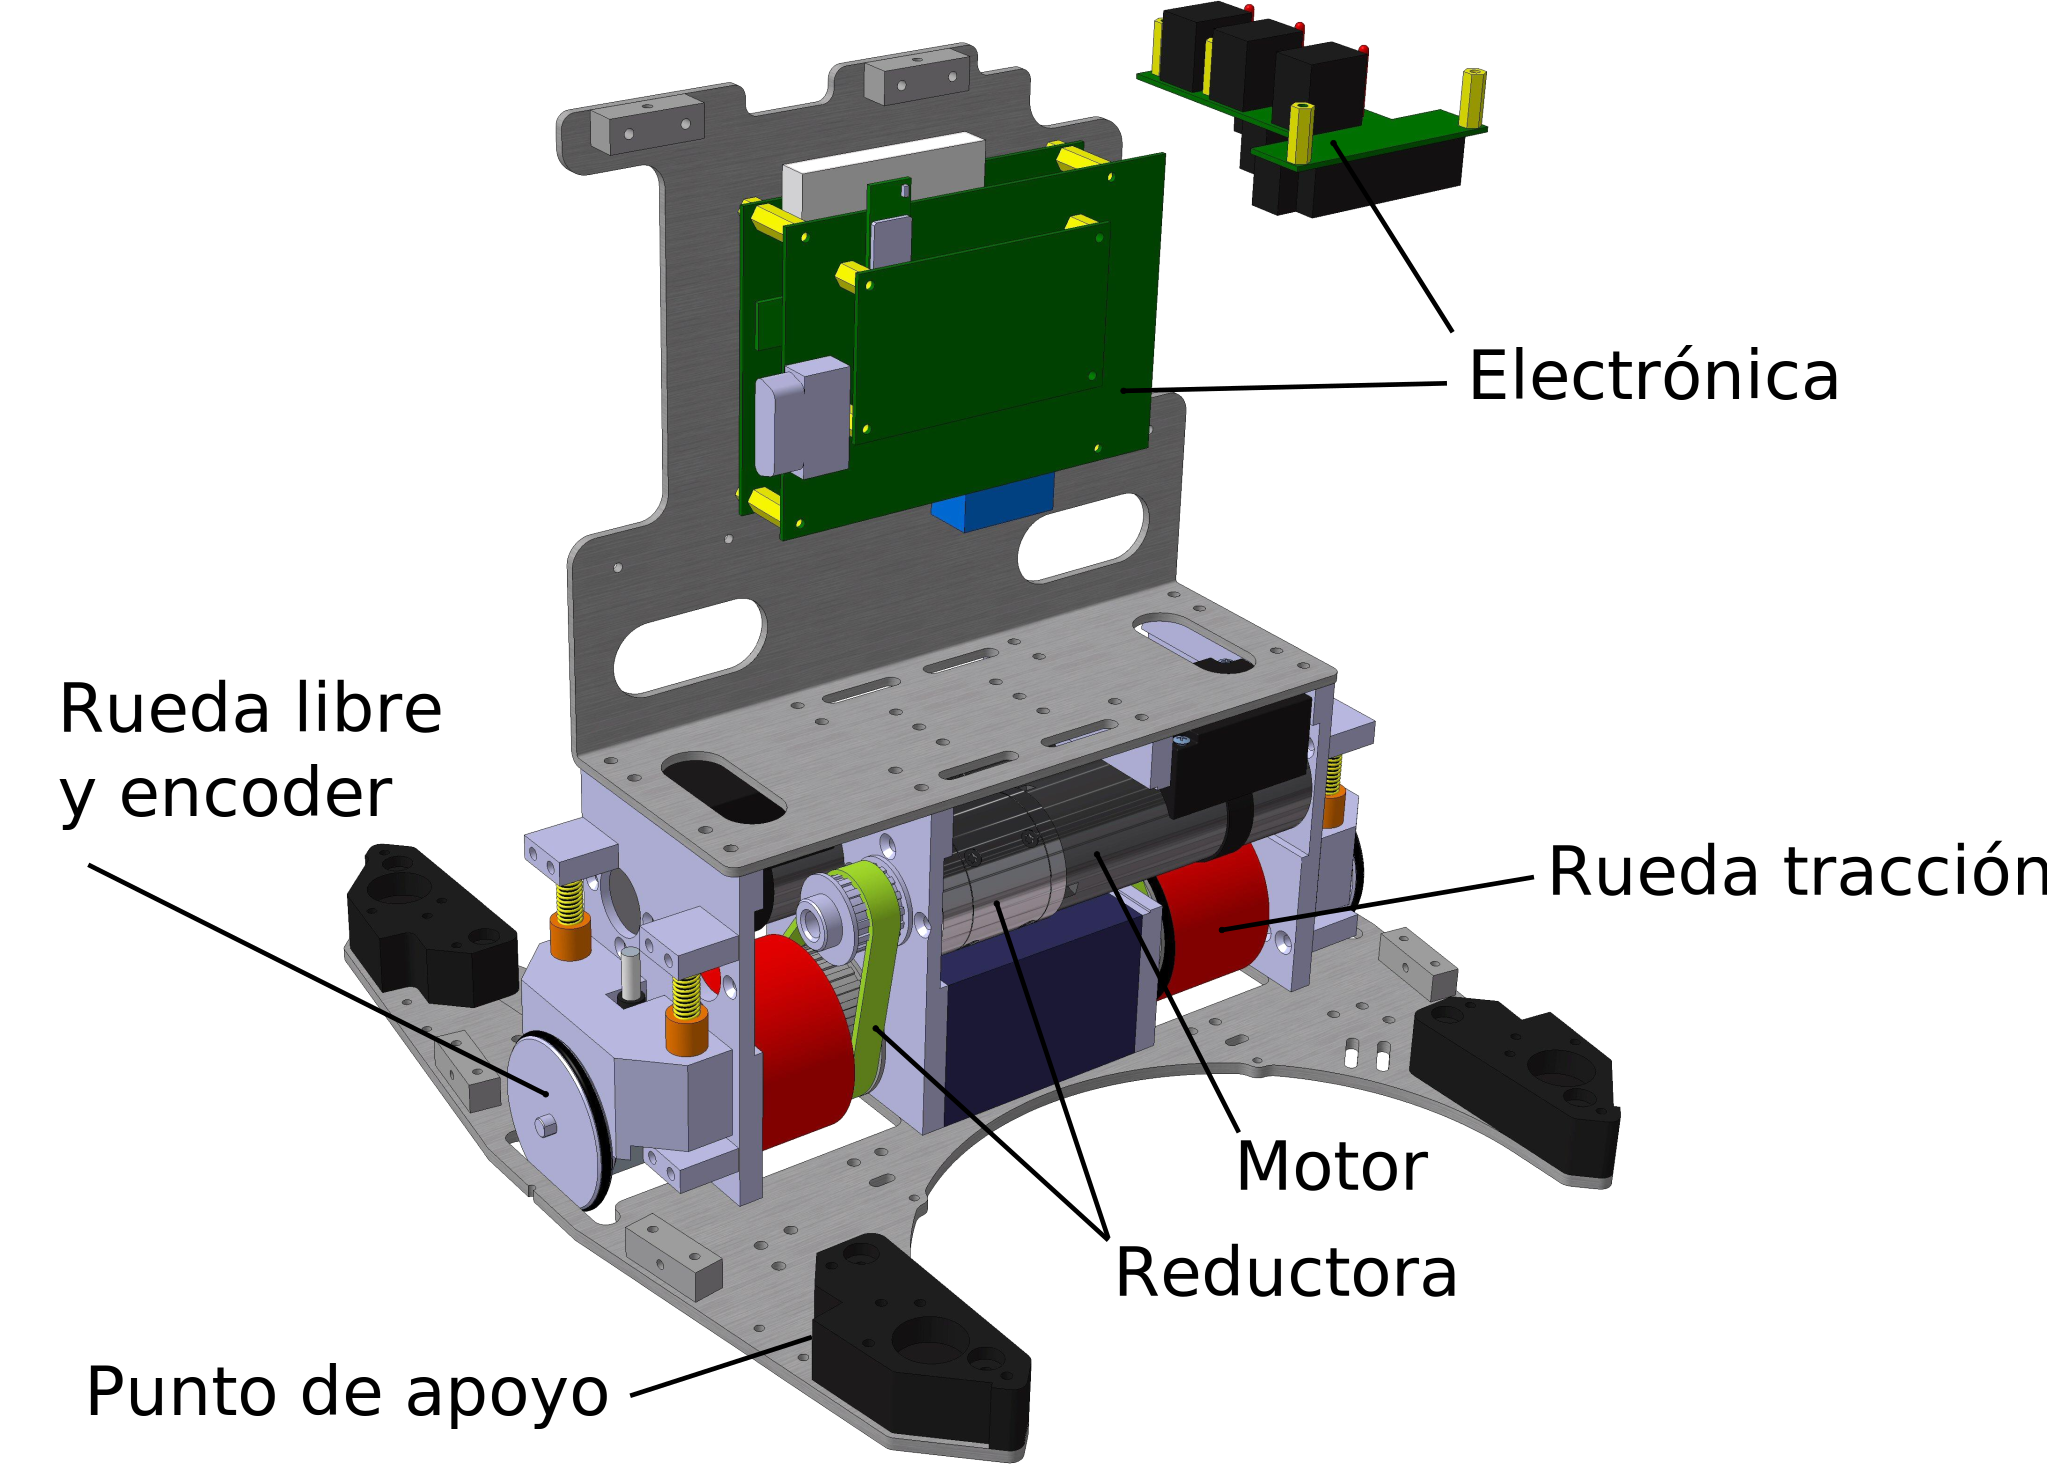
\includegraphics[width=.5\textwidth]{plataforma_partes_1}
\includegraphics[width=.35\textwidth]{plataforma_partes_2}
\caption[]{Elementos de la plataforma rob�tica base}
\label{fig_plataforma_partes_resumen}
\end{figure}

La \textbf{evitaci�n de obst�culos} se realiza a partir de sensores de distancia situados en las caras del robot (ver figura \ref{fig_plataforma_partes_resumen}) y a partir de un \emph{sistema de balizamiento} que hace uso de los soportes y espacios destinados a las balizas de la competici�n Eurobot. �ste sistema est� compuesto por un sensor tipo faro situado en el robot y balizas reflectantes situadas en el oponente (ver figura \ref{fig_plataforma_partes_resumen}). Y est� espec�ficamente desarrollado para medir la distancia y �ngulo de los oponentes relativo a la posici�n del la plataforma rob�tica.

% (BALIZA)
El sistema de baliza tipo faro se compone de un sensor giratorio y de una o varias balizas cil�ndricas reflectantes. El sensor gira sobre el plano $xy$ y emite una luz que es reflejada por balizas reflectantes cuando el sensor se encuentra enfrentado con ellas.  La medida de distancia se basa en el principio por el cual un objeto cercano se ve m�s grande que uno lejano. De forma que a una distancia cercana le corresponde un �ngulo relativo de detecci�n $\alpha_d$ mayor que el de una distancia m�s lejana. Por otro lado, la medida de �ngulo se obtiene a partir del �ngulo durante el cual se detecta la baliza reflectante.

% HW
El desarrollo HW propuesto, implementa una \textbf{arquitectura HW} que contempla la implementaci�n tanto de la plataforma rob�tica, como de los sistemas mec�nicos del robot. Se basa un sistema embebido basado en microcontroladores dsPIC que tiene sus recursos repartidos entre, la implementaci�n de la plataforma rob�tica base y de los sistema mec�nicos. Debido a que los recursos destinados a los sistemas mec�nicos dependen de la tem�tica de la prueba, la arquitectura tiene una interfaz I2C destinada expansi�n de recursos de entrada/salida (E/S) y a la implementaci�n de un procesamiento distribuido.

Por otro lado, la arquitectura HW tiene una interfaz de depuraci�n RS-232 a trav�s de la cual poder controlar, monitorizar y probar el hardware y el software desarrollado. Esta interfaz forma una cadena serie con el resto de microcontroladores que permite acceder a cualquiera de ellos mediante un \emph{bypass} del los datos. Adem�s, la arquitectura cuenta con una interfaz inal�mbrica Bluetooth, mediante la cual se implementa la \textbf{comunicaci�n con la baliza tipo faro y el robot secundario}. Dependiendo de las caracter�sticas del robot, esta arquitectura HW ha sido implementada en una o varias tarjetas electr�nicas, como se muestra en varios ejemplos de robots desarrollados.


% (ver figura \ref{fig_hardware_arquitectura_principal_resumen}).

%\begin{figure}[ht]
%\centering
%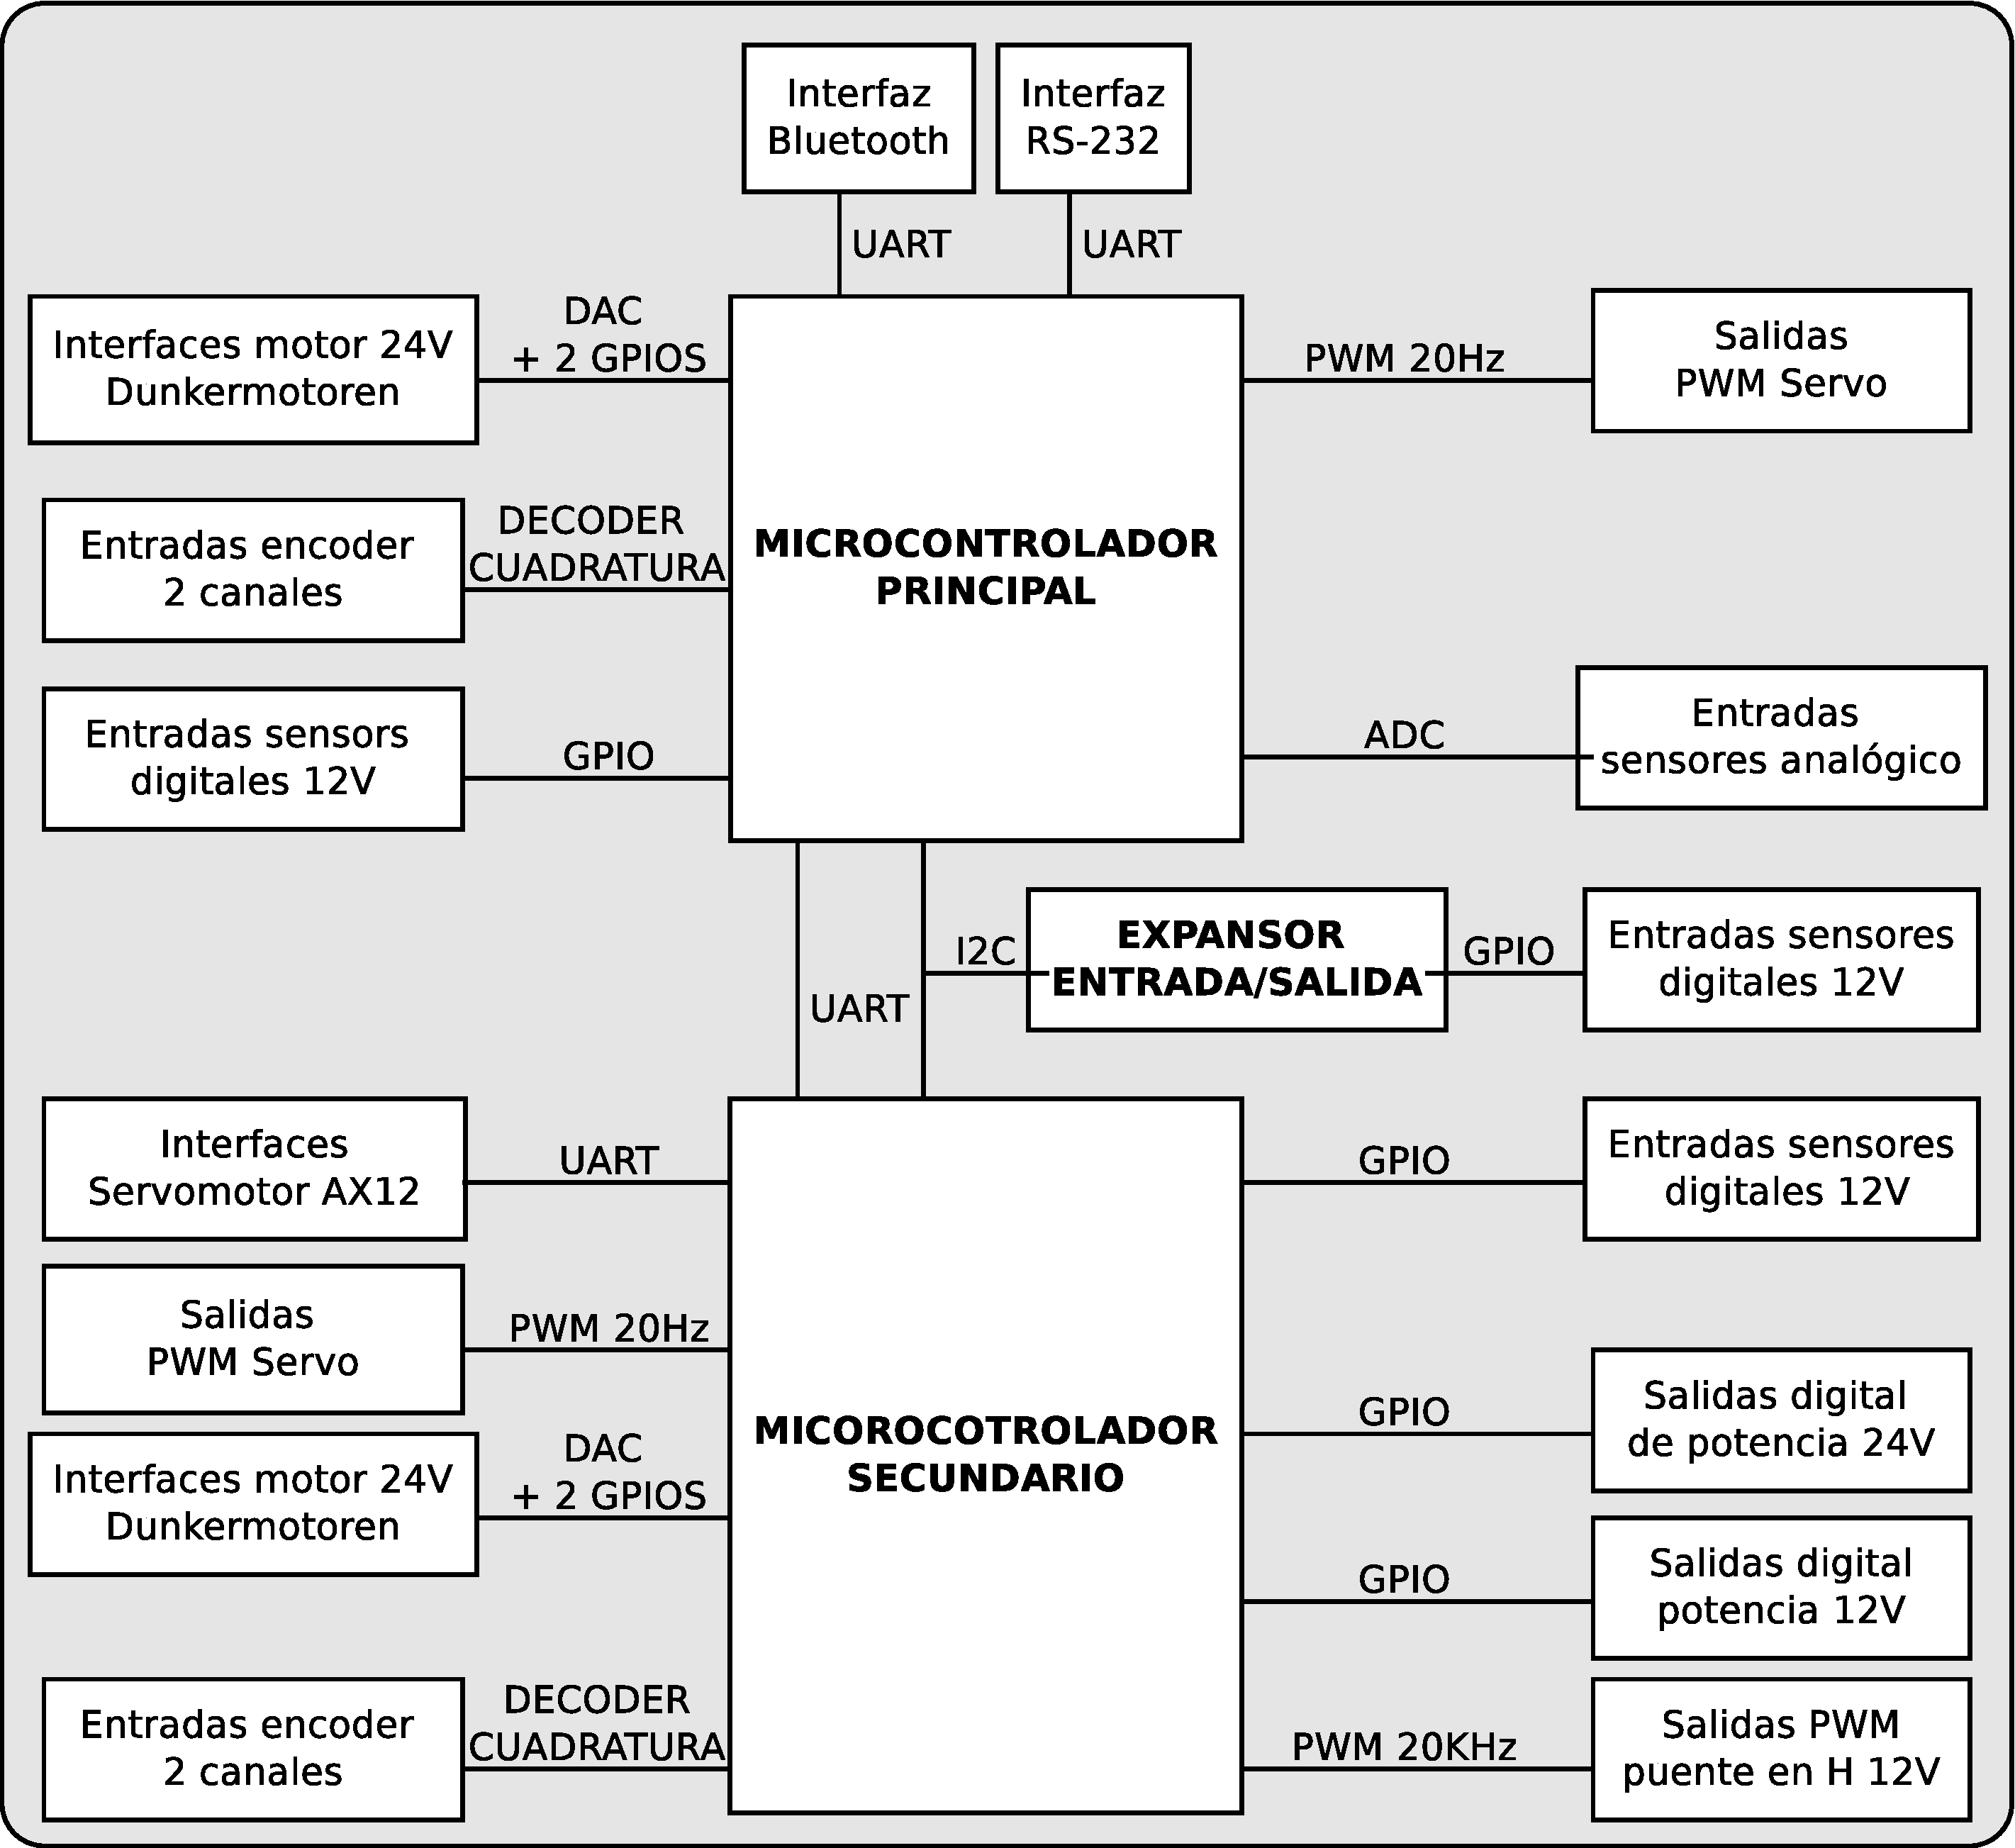
\includegraphics[width=.9\textwidth]{hardware_arquitectura_principal}
%\caption[]{Arquitectura hardware desarrollada}
%\label{fig_hardware_arquitectura_principal_resumen}
%\end{figure}


% SW
Se describe un desarrollo SW que implementa una \textbf{arquitectura SW} cuya estructura incluye la implementaci�n funcional de la plataforma rob�tica, los sistemas mec�nicos y las funcionalidades propias de la tem�tica y estrategia de juego del robot de Eurobot. Se tratan ejemplos de robots desarrollados que implementan esta arquitectura SW.

La implementaci�n SW de la plataforma rob�tica se ha realizado a partir de las librer�as Aversive \cite{aversive_src}, desarrolladas por el equipo de Eurobot Microb Technology \cite{microb}. Las librer�as Aversive constituyen un marco de trabajo para el desarrollo de sistemas basados en microcontroladores AVR de Atmel. A partir de estas librer�as se crearon las librer�as Aversive4dspic, una migraci�n de las librer�as Aversive a microcontroladores dsPIC de Microchip, utilizados por el HW desarrollado. 

La arquitectura SW propuesta se organiza en capas o m�dulos funcionales, de forma que aquellos de nivel superior implementan funciones m�s abstractas que los inferiores. El m�dulo \emph{plataforma rob�tica} incluye las funcionalidades de desplazamiento, localizaci�n y evitaci�n de obst�culos. Al mismo nivel, se encuentra el m�dulo \emph{sistemas mec�nicos} encargado de controlar los mecanismos utilizados por el robot para manipular los elementos de juego. Ambos m�dulos se integran y se sincronizan en la capa de \emph{tem�tica de juego} para implementar funcionalidades propias de la tem�tica de Eurobot. Por �ltimo, la capa \emph{estrategia de juego} decide cuando y que acciones del juego realizar en cada momento para jugar un partido de Eurobot.

%\begin{description}
%\item \textbf{Drivers de dispositivos HW}

%Capa de menor nivel que permite abstraer los m�dulos o dispositivos HW del robot, como m�dulos de comunicaci�n del microcontrolador (UART, I2C, SPI, ...) o dispositivos externos a �ste como servomotores, o drivers en puente en H para el control de motores.

%\item \textbf{Plataforma rob�tica base}

%M�dulo que implementa las funcionalidades de la plataforma rob�tica base: control de posici�n, odometr�a, gesti�n de trayectorias y evitaci�n de obst�culos.

%\item \textbf{Sistemas mec�nicos}

%M�dulo que abstrae el control de los diferentes sistemas mec�nicos del robot mediante los cuales se manipulan los elementos del  juego. Este m�dulo a su vez se encuentra dividido en varios niveles, representados en el microcontrolador esclavo del robot principal de la figura \ref{fig_sw_diagrama_bloques_resumen}).

%\item \textbf{Tem�tica de juego}

%Nivel que integra toda la funcionalidad de los niveles inferiores y sistemas externos, como la baliza y el robot secundario, para implementar las funcionalidades del robot relativas a la prueba de Eurobot y a la navegaci�n del robot por el campo de juego.

%\item \textbf{Estrategia de juego}

%Esta capa implementa la estrategia de juego de un partido as� como las diferentes fases de las que se compone un partido.

%\item \textbf{Linea de comandos}

%Capa de mayor nivel que permite ejecutar comandos de cualquier m�dulo o nivel. De esta forma durante el desarrollo de las diferentes capas o m�dulos, las funcionalidades de �stas pueden ser probadas por partes y verificar su correcto funcionamiento.

%\end{description}

%\begin{figure}[t]
%\centering
%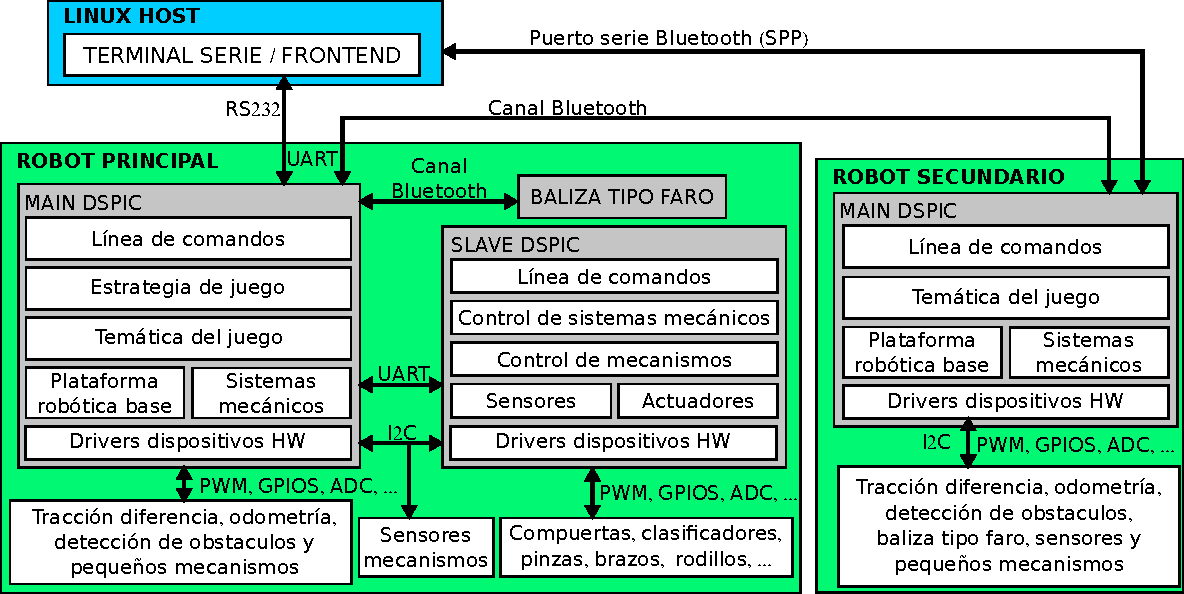
\includegraphics[width=\textwidth]{sw_diagrama_bloques}
%\caption[]{Diagrama de bloques software del robot principal y secundario}
%\label{fig_sw_diagrama_bloques_resumen}
%\end{figure}

%La figura \ref{fig_sw_diagrama_bloques_resumen} representa la implementaci�n de la arquitectura el caso de dos robots: un robot principal y uno secundario se muestra en la figura \ref{fig_sw_diagrama_bloques_resumen}. Ambos robots implementan la misma arquitectura. El robot principal, implementa la arquitectura mediante dos microcontroladores, mientras que el secundario utiliza �nicamente un �nico microcontrolador.

Por �ltimo, el desarrollo SW incluye adem�s un \textbf{simulador de los robots y del campo de juego}. Este simulador se implementa a partir de la compilaci�n del c�digo fuente de los robots en un \emph{host} GNU/Linux y de la emulaci�n del HW y elementos mec�nicos del robot. El entorno de simulaci�n permite visualizar los movimientos de los robots sobre un campo de juego virtual y simular robots oponentes.






%%% Local Variables:
%%% TeX-master: "../book"
%%% End:


       % EDIT this file

% Now include toc and list of figures+tables
%%%%%%%%%%%%%%%%%%%%%%%%%%%%%%%%%%%%%%%%%%%%%%%%%%%%%%%%%%%%%%%%%%%%%%%%%%%
%
% Generic template for TFC/TFM/TFG/Tesis
%
% $Id: toc+lof+lot.tex,v 1.8 2014/01/08 22:56:06 macias Exp $
%
% By:
%  + Javier Mac�as-Guarasa. 
%    Departamento de Electr�nica
%    Universidad de Alcal�
%  + Roberto Barra-Chicote. 
%    Departamento de Ingenier�a Electr�nica
%    Universidad Polit�cnica de Madrid   
% 
% Based on original sources by Roberto Barra, Manuel Oca�a, Jes�s Nuevo,
% Pedro Revenga, Fernando Herr�nz and Noelia Hern�ndez. Thanks a lot to
% all of them, and to the many anonymous contributors found (thanks to
% google) that provided help in setting all this up.
%
% See also the additionalContributors.txt file to check the name of
% additional contributors to this work.
%
% If you think you can add pieces of relevant/useful examples,
% improvements, please contact us at (macias@depeca.uah.es)
%
% Copyleft 2013
%
%%%%%%%%%%%%%%%%%%%%%%%%%%%%%%%%%%%%%%%%%%%%%%%%%%%%%%%%%%%%%%%%%%%%%%%%%%%

\hypersetup{linkcolor=\mytoclinkcolor}
\tableofcontents

\hypersetup{linkcolor=\myloflinkcolor}
\listoffigures
                          
\hypersetup{linkcolor=\mylotlinkcolor}
\listoftables

\hypersetup{linkcolor=\mylinkcolor}

%%% Local Variables:
%%% TeX-master: "../book"
%%% End:
                 % DO NOT TOUCH THIS LINE!

% If you want to include additional listings, you can use the float
% package. As an example, I include here the listing of source code
% snippets (you have some examples in appendix/manual.tex)
%%%%%%%%%%%%%%%%%%%%%%%%%%%%%%%%%%%%%%%%%%%%%%%%%%%%%%%%%%%%%%%%%%%%%%%%%%%
%
% Generic template for TFC/TFM/TFG/Tesis
%
% $Id: extralistings.tex,v 1.3 2014/01/08 22:56:05 macias Exp $
%
% By:
%  + Javier Mac�as-Guarasa. 
%    Departamento de Electr�nica
%    Universidad de Alcal�
%  + Roberto Barra-Chicote. 
%    Departamento de Ingenier�a Electr�nica
%    Universidad Polit�cnica de Madrid   
% 
% Based on original sources by Roberto Barra, Manuel Oca�a, Jes�s Nuevo,
% Pedro Revenga, Fernando Herr�nz and Noelia Hern�ndez. Thanks a lot to
% all of them, and to the many anonymous contributors found (thanks to
% google) that provided help in setting all this up.
%
% See also the additionalContributors.txt file to check the name of
% additional contributors to this work.
%
% If you think you can add pieces of relevant/useful examples,
% improvements, please contact us at (macias@depeca.uah.es)
%
% Copyleft 2013
%
%%%%%%%%%%%%%%%%%%%%%%%%%%%%%%%%%%%%%%%%%%%%%%%%%%%%%%%%%%%%%%%%%%%%%%%%%%%

% Include the list of source code listings (if this is the case)
\hypersetup{linkcolor=\myothertoclinkcolor}
\ifthenelse{\equal{\mybooklanguage}{english}}
{
  \listof{codefloat}{List of source code listings}
}
{
  \listof{codefloat}{�ndice de listados de c�digo fuente}    
}
\hypersetup{linkcolor=\mylinkcolor}

%%% Local Variables:
%%% TeX-master: "../book"
%%% End:
               % Edit this file or
                                              % comment it out

% Now include acronyms (if this is the case)
%%%%%%%%%%%%%%%%%%%%%%%%%%%%%%%%%%%%%%%%%%%%%%%%%%%%%%%%%%%%%%%%%%%%%%%%%%%
%
% Generic template for TFC/TFM/TFG/Tesis
%
% $Id: acronymsgl.tex,v 1.5 2014/01/08 22:56:03 macias Exp $
%
% By:
%  + Javier Mac�as-Guarasa. 
%    Departamento de Electr�nica
%    Universidad de Alcal�
%  + Roberto Barra-Chicote. 
%    Departamento de Ingenier�a Electr�nica
%    Universidad Polit�cnica de Madrid   
% 
% Based on original sources by Roberto Barra, Manuel Oca�a, Jes�s Nuevo,
% Pedro Revenga, Fernando Herr�nz and Noelia Hern�ndez. Thanks a lot to
% all of them, and to the many anonymous contributors found (thanks to
% google) that provided help in setting all this up.
%
% See also the additionalContributors.txt file to check the name of
% additional contributors to this work.
%
% If you think you can add pieces of relevant/useful examples,
% improvements, please contact us at (macias@depeca.uah.es)
%
% Copyleft 2013
%
%%%%%%%%%%%%%%%%%%%%%%%%%%%%%%%%%%%%%%%%%%%%%%%%%%%%%%%%%%%%%%%%%%%%%%%%%%%

% This file shows some examples for glossary terms

%%%%%%%%%%%%%%%%%%%%%%%%%%%%%%%%%%%%%%%%%%%%%%%%%%%%%%%%%%%%%%%%%%%%%%%%%%%
% BEGIN example of glossary terms definition
%
\newacronym{HMI}{HMI}{Human-Machine Interfaces}
\newacronym{ETTS}{ETTS}{Emotional Text To Speech}
\newacronym{TTS}{TTS}{Text To Speech}
\newacronym{PSOLA}{PSOLA}{Pitch Synchronous OverLap Add}
\newacronym{TDPSOLA}{TD-PSOLA}{Time Domain Pitch Synchronous OverLap Add}
\newacronym{AI}{AI}{Artificial Intelligenge}

\newacronym{SPSS}{SPSS}{Statistical Parametric Speech Synthesis}
\newacronym{VC}{VC}{Voice Conversion}
\newacronym{US}{US}{Unit Selection}
\newacronym{HMM}{HMM}{Hidden Markov Model}
\newacronym{LSP}{LSP}{Line Spectral Pairs}
\newacronym{LPC}{LPC}{Linear Prediction Coefficiens}
\newacronym{LSF}{LSF}{Line Spectral Frequencies}
\newacronym{F0}{F0}{Fundamental Frequency}
\newacronym{MCEP}{MCEP}{Mel Cepstral Coefficients}
\newacronym{MGCEP}{MGCEP}{Mel Generalized Cepstral Coefficients}
\newacronym{MFCC}{MFCC}{Mel Frequency Cepstrum Coefficients}
\newacronym{ASR}{ASR}{Automatic Speech Recognition}
\newacronym{MDL}{MDL}{Minimum Description Length Criterion}
\newacronym{MSD}{MSD}{Multi Space Probability Distributions}
\newacronym{HSMM}{HSMM}{Hidden Semi-Markov Models}
\newacronym{ML}{ML}{Maximum Likelihood}
\newacronym{MLSA}{MLSA}{Mel Log Spectrum Approximation}
\newacronym{MAP}{MAP}{Maximum A Posteriori} 
\newacronym{MLLR}{MLLR}{Maximum Likelihood Linear Regression}
\newacronym{CSMAPLR}{CSMAPLR}{Constrain Structural MAP Linear Regression}
\newacronym{AV}{AV}{Average Voice}

\newacronym{ANN}{ANN}{Artificial Neural Network}

\newacronym{NIST}{NIST}{National Institute of Technology}
\newacronym{SES}{SES}{Spanish Expressive Speech}
\newacronym{EMODB}{EMODB}{Berlin Database of Emotional Speech}

\newacronym{FAUAIBO}{FAU-AIBO}{FAU AIBO Emotion Corpus}

\newacronym{SEV}{SEV}{Spanish Expressive Voices}
\newacronym{AER}{AER}{Automatic Emotion Recognition}
\newacronym{UBEC}{UBEC}{Universal Background Emotion Codebook}

\newacronym{STRAIGHT}{STRAIGHT}{Speech Transformation and Representation using Adaptive Interpolation of weiGHTed spectrum}


\newacronym{DBN}{DBN}{Dynamic Bayesian Network}
\newacronym{SQ}{SQ}{Speech Quality}
\newacronym{EIR}{EIR}{Emotion Identification Rate}
\newacronym{SIR}{SIR}{Speaker Identification Rate}
\newacronym{ES}{ES}{Emotional Strength}

\newacronym{ACCCHARS}{��������������}{Long ��������������}

% In the future version of texlive, we will be able to use longplural
% and shortplural. Right now we must use \newglossaryentry.
%\newacronym[longplural={Systems on a Chip},shortplural={SOCs}]{SOC}{SOC}{System on a Chip}
\newglossaryentry{SOC}{type=\acronymtype,
        name={SOC},
        symbol={},
        sort=soc,
        plural={SOCs},
        firstplural={Systems on a Chip (SOCs)},
        description={System on a Chip},
        descriptionplural={Systems on a Chip}}

%
% END example of glossary terms definition
%%%%%%%%%%%%%%%%%%%%%%%%%%%%%%%%%%%%%%%%%%%%%%%%%%%%%%%%%%%%%%%%%%%%%%%%%%%

% You can change the way the entries appear the first time they are
% used. I've used italics by default
\defglsdisplayfirst[\acronymtype]{\textit{#1}} % EDIT this if required

% This may lead to problems... I don't know how to fix it in case the
% column for acronym is wider than 0.3\linewidth
\setlength{\glsdescwidth}{0.7\linewidth}       % EDIT this if required

% Set language specific definitions...
\ifthenelse{\equal{\mybooklanguage}{english}}
{
\printglossary[type=\acronymtype,style=super,nonumberlist=true,title=List of Acronyms,toctitle=List of Acronyms]
\addcontentsline{toc}{chapter}{List of Acronyms}
}
{
\printglossary[type=\acronymtype,style=super,nonumberlist=true,title=Lista de acr�nimos,toctitle=Lista de acr�nimos]
\addcontentsline{toc}{chapter}{Lista de acr�nimos}
}


%%% Local Variables:
%%% TeX-master: "../book"
%%% End:


               % EDIT this file or
                                              % comment it out if you do
                                              % not use acronyms

% Now include symbols (if this is the case)
%%%%%%%%%%%%%%%%%%%%%%%%%%%%%%%%%%%%%%%%%%%%%%%%%%%%%%%%%%%%%%%%%%%%%%%%%%%
%
% Generic template for TFC/TFM/TFG/Tesis
%
% $Id: symbolsgl.tex,v 1.5 2014/01/08 22:56:07 macias Exp $
%
% By:
%  + Javier Mac�as-Guarasa. 
%    Departamento de Electr�nica
%    Universidad de Alcal�
%  + Roberto Barra-Chicote. 
%    Departamento de Ingenier�a Electr�nica
%    Universidad Polit�cnica de Madrid   
% 
% Based on original sources by Roberto Barra, Manuel Oca�a, Jes�s Nuevo,
% Pedro Revenga, Fernando Herr�nz and Noelia Hern�ndez. Thanks a lot to
% all of them, and to the many anonymous contributors found (thanks to
% google) that provided help in setting all this up.
%
% See also the additionalContributors.txt file to check the name of
% additional contributors to this work.
%
% If you think you can add pieces of relevant/useful examples,
% improvements, please contact us at (macias@depeca.uah.es)
%
% Copyleft 2013
%
%%%%%%%%%%%%%%%%%%%%%%%%%%%%%%%%%%%%%%%%%%%%%%%%%%%%%%%%%%%%%%%%%%%%%%%%%%%

% These ones for the symbols glossary

%%%%%%%%%%%%%%%%%%%%%%%%%%%%%%%%%%%%%%%%%%%%%%%%%%%%%%%%%%%%%%%%%%%%%%%%%%%
% BEGIN example of symbols definition
%
\newglossaryentry{ohm}{type=symbols,
        name={\ensuremath{\Omega}},
        symbol={\ensuremath{\Omega}}, 
        sort=ohm,
        description=unit of electrical resistance}

\newglossaryentry{angstrom}{type=symbols,
        name={\AA},
        symbol={\AA},
        sort=angstrom,
        description={non-SI unit of length}}

\newglossaryentry{xdet}{type=symbols,
        name={\ensuremath{x(t)}},
        symbol={\ensuremath{x(t)}},
        sort=xdet,
        description={Audio signal}}

\newglossaryentry{xidet}{type=symbols,
        name={\ensuremath{x_i(t)}},
        symbol={\ensuremath{x_i(t)}},
        sort=xidet,
        description={Audio signal captured at microphone $i$}}

%
% END example of symbols definition
%%%%%%%%%%%%%%%%%%%%%%%%%%%%%%%%%%%%%%%%%%%%%%%%%%%%%%%%%%%%%%%%%%%%%%%%%%%

% Set language specific definitions...
\ifthenelse{\equal{\mybooklanguage}{english}}
{
  \printglossary[type=symbols,style=super,nonumberlist=true,title=List of Symbols,toctitle=List of Symbols]
  \addcontentsline{toc}{chapter}{List of Symbols}
}
{
  \printglossary[type=symbols,style=super,nonumberlist=true,title=Lista de s�mbolos,title=Lista de s�mbolos,toctitle=Lista de s�mbolos]
  \addcontentsline{toc}{chapter}{Lista de s�mbolos}
}


%%% Local Variables:
%%% TeX-master: "../book"
%%% End:
                 % EDIT this file or
                                              % comment it out if you do
                                              % not use acronyms

%
% END within-document configuration, frontpage and cover pages generation
%%%%%%%%%%%%%%%%%%%%%%%%%%%%%%%%%%%%%%%%%%%%%%%%%%%%%%%%%%%%%%%%%%%%%%%%%%%


%%%%%%%%%%%%%%%%%%%%%%%%%%%%%%%%%%%%%%%%%%%%%%%%%%%%%%%%%%%%%%%%%%%%%%%%%%%
% Now start text and numbering for mainmatter (chapter+appendices)
%%%%%%%%%%%%%%%%%%%%%%%%%%%%%%%%%%%%%%%%%%%%%%%%%%%%%%%%%%%%%%%%%%%%%%%%%%%
\mainmatter                                       % DO NOT TOUCH THIS LINE!
\deactivatetilden                                 % DO NOT TOUCH THIS LINE!


%%%%%%%%%%%%%%%%%%%%%%%%%%%%%%%%%%%%%%%%%%%%%%%%%%%%%%%%%%%%%%%%%%%%%%%%%%%
%%%%%%%%%%%%%%%%%%%%%%%%%%%%%%%%%%%%%%%%%%%%%%%%%%%%%%%%%%%%%%%%%%%%%%%%%%%
%%%%%%%%%%%%%%%%%%%%%%%%%%%%%%%%%%%%%%%%%%%%%%%%%%%%%%%%%%%%%%%%%%%%%%%%%%%
%%%%%%%%%%%%%%%%%%%%%%%%%%%%%%%%%%%%%%%%%%%%%%%%%%%%%%%%%%%%%%%%%%%%%%%%%%%
%%%%%%%%%%%%%%%%%%%%%%%%%%%%%%%%%%%%%%%%%%%%%%%%%%%%%%%%%%%%%%%%%%%%%%%%%%%
%%%%%%%%%%%%%%%%%%%%%%%%%%%%%%%%%%%%%%%%%%%%%%%%%%%%%%%%%%%%%%%%%%%%%%%%%%%
%%%%%%%%%%%%%%%%%%%%%%%%%%%%%%%%%%%%%%%%%%%%%%%%%%%%%%%%%%%%%%%%%%%%%%%%%%%
% BEGIN Normal chapters. Edit/modify all within this section
%
% I don't recommend it, but if you want to define "parts", use this...
% BEWARE: I didn't write the english dependent code
%\part*{Memoria}
%\label{part:memoria}

%%%%%%%%%%%%%%%%%%%%%%%%%%%%%%%%%%%%%%%%%%%%%%%%%%%%%%%%%%%%%%%%%%%%%%%%%%%
%
% Generic template for TFC/TFM/TFG/Tesis
%
% $Id: introduccion.tex,v 1.6 2014/02/11 11:00:06 macias Exp $
%
% By:
%  + Javier Mac�as-Guarasa. 
%    Departamento de Electr�nica
%    Universidad de Alcal�
%  + Roberto Barra-Chicote. 
%    Departamento de Ingenier�a Electr�nica
%    Universidad Polit�cnica de Madrid   
% 
% Based on original sources by Roberto Barra, Manuel Oca�a, Jes�s Nuevo,
% Pedro Revenga, Fernando Herr�nz and Noelia Hern�ndez. Thanks a lot to
% all of them, and to the many anonymous contributors found (thanks to
% google) that provided help in setting all this up.
%
% See also the additionalContributors.txt file to check the name of
% additional contributors to this work.
%
% If you think you can add pieces of relevant/useful examples,
% improvements, please contact us at (macias@depeca.uah.es)
%
% Copyleft 2013
%
%%%%%%%%%%%%%%%%%%%%%%%%%%%%%%%%%%%%%%%%%%%%%%%%%%%%%%%%%%%%%%%%%%%%%%%%%%%

\chapter{Introducci�n al proyecto}
\label{cha:introduccion}

\begin{FraseCelebre}
  \begin{Frase}
    Desocupado lector, sin juramento me podr�s creer que quisiera que este
    libro [...] fuera el m�s hermoso, el m�s gallardo y m�s discreto que
    pudiera imaginarse\footnote{Tomado de ejemplos del proyecto \texis{}.}.
  \end{Frase}
  \begin{Fuente}
    Miguel de Cervantes, Don Quijote de la Mancha
  \end{Fuente}
\end{FraseCelebre}


\section{Presentaci�n}
\label{sec:presentacion}

Este trabajo de fin de carrera trata sobre el desarrollo de robots para la competici�n de robots Eurobot \cite{eurobot}. Pretende ser un manual de referencia para todo aquel que quiera construir un robot para participar en Eurobot\footnote{O para desarrollar un robot de similares caracter�sticas para cualquier otro cometido}. Todo lo que se expone en este libro esta se sustenta en la experiencia adquirida en el desarrollo de robots participantes en Eurobot entre los a�os 2003 y 2015. Especialmente en el periodo entre 2010 y 2015.

\section{La competici�n Eurobot}
\label{sec:la_competicion_eurobot}

Eurobot es un concurso internacional de rob�tica creado en 1998 a partir de la Copa de Francia de la rob�tica \cite{cdr} (Coupe de France de robotique). El concurso est� abierto a equipos de j�venes, organizados ya sea en proyectos de estudiantes o en clubes independientes. Eurobot se lleva a cabo en Europa, pero da la bienvenida a los equipos de todos los continentes.

Cada a�o, las reglas se publican alrededor de octubre. Los equipos tienen entonces varios meses para dise�ar y construir sus robots y competir entre abril y junio en el concurso nacional, en el cual se pueden seleccionar s�lo 3 equipos por pa�s. Los mejores equipos de cada pa�s se reunir�n despu�s para competir en las finales de Eurobot.

Las reglas cambian cada a�o, sin embargo, la base es siempre la misma:

\begin{itemize}
\item Los robots tienen aproximadamente el tama�o de un cubo de 30 cm.
\item El campo de juego tiene una dimensi�n de 2 metros de ancho y 3 metros de largo.
\item El juego tiene 90 segundos de duraci�n.
\item Los robots tienen que llevar a cabo varias tareas en el campo con el fin de ganar tantos puntos como sea posible.
\item Los robots tienen que evitarse unos a otros y evitar los choques.
\item Los robots son completamente aut�nomos y deben hacer todas las acciones por ellos mismos.
\end{itemize}

Tal y como est� dise�ado, Eurobot constituye un reto de ingenier�a que permite a alumnos de electr�nica, mec�nica e inform�tica aplicar sus conocimientos o ampliarlos y compartirlos. Tambi�n hace, por ejemplo, que alumnos de electr�nica aprendan mec�nica o inform�tica o ambos campos o todos. Dada la complejidad de los robots suelen ser construidos por equipo formados de al menos 2 personas, lo cual implica cierta organizaci�n, divisi�n de tareas y trabajo en equipo. Un equipo numeroso permite desarrollar robots con partes m�s especializadas pero implica una gesti�n y coordinaci�n mayor. Por otro lado, Eurobot implica confeccionar un producto completo, original y funcional desde cero\footnote{No siempre se ha de empezar desde cero, un desarrollo modular y estructurado permite partir de una base m�nima.} (o como dir�amos en Ingl�s \emph{from scratch}) en cosa de 6 o 7 meses. Esto implica una elecci�n y compra de materiales, componentes, dise�o electr�nico y mec�nico, construcci�n de prototipos, desarrollo de software, ... y en definitiva una gesti�n del tiempo. Tiempo que suele escasear porque los participantes, generalmente alumnos, disponen de �l escasamente\footnote{Y parece ser que menos a�n con los actuales planes de estudios Bolonia}.

La comunidad de Eurobot se comunica principalmente a trav�s de sus foros\cite{foros_eurobot}. Hay tres foros principales: un foro relacionado con las reglas de cada a�o, el foro de Eurobot Open\cite{foro_eurobot_open} y el foro de la Copa de Francia de la rob�tica\cite{foro_copa_francia}. Este �ltimo es el foro m�s activo dado que la Copa nacional de Francia es la de mayor tradici�n y la que re�ne el mayor numero de participantes. Este foro, aunque est� escrito en franc�s, es el que acumula la mayor�a de la informaci�n acerca de la competici�n y de temas t�cnicos. Adem�s, cada equipo suele tener una p�gina web, blog o canal de Youtube donde comparte los avances de los robots que construyen cada a�o.

Eurobot est� organizada gracias la asociaci�n internacional de Eurobot y a la asociaci�n francesa \emph{Planet Sciences}\cite{planet_sciences} y a muchas otras asociaciones, escuelas, universidades y personas voluntarias de los pa�ses participantes. Es incre�ble la cantidad de personas que apoyan Eurobot y trabajan de forma voluntaria sin ninguna remuneraci�n m�s que la satisfacci�n de estar implicados y formar parte de esta fiesta que es Eurobot. Y esto incluye a los participantes, ya que ganar Eurobot no implica ning�n premio econ�mico. En total, un mont�n de gente que trabaja para disfrutar y divertirse con la rob�tica.


\section{El equipo \emph{Eurobotics Engineering}, historia y antecedentes}
\label{sec:equipo_eurobotics}

\emph{Eurobotics Engineering}\cite{arc_robots} es un equipo participante en Eurobot formado por entusiastas de la rob�tica. Est� formado por estudiantes de la Universidad de Alcal� (UAH): ingenieros de telecomunicaci�n, de electr�nica, de telem�tica y de electr�nica industrial.

La historia de este equipo se remonta al a�o 2003, a�o en el que el Departamento de Electr�nica de la UAH decide montar un equipo patrocinado a partir de la iniciativa de un grupo de alumnos de participar en Eurobot 2002. Los integrantes del equipo se renuevan cada a�o excepto algunos que se mantienen. Exceptuando el a�o 2009, el resto de a�os el equipo particip� en Eurobot. En el a�o 2010 Diego Salazar y Javier Bali�as crean el equipo de Eurobot llamado \emph{Eurobotics Engineering} y en el a�o 2011, junto con Nilo Masias, fundaron y la Asociaci�n de Rob�tica de Coslada (ARC).

El equipo Eurobot Engineering particip� en Eurobot desde el a�o 2010 hasta el a�o 2015 (exceptuando el a�o 2013). Durante estos a�os ha contado con el apoyo del Dpto. de Electr�nica de la Universidad de la UAH\cite{depeca,uah} y el Ayuntamiento de Coslada, adem�s del patrocinio de Ayudas Hidr�ulicas\cite{ayudas_hidraulicas}, Carpinter�a Ingl�s, Ro-botica\cite{ro_botica} (2010-2012), el Consejo de estudiantes de la UAH\cite{consejo_de_estudiantes} (2014-2015) y Mobile Minds\cite{mobile_minds} (2015).


\section{La rob�tica educativa}
\label{sec:robotica_educativa}

A d�a de hoy la rob�tica constituye una herramienta educativa muy potente. Permite aprender y poner en practica diferentes ramas de la ciencia. Lo hace a trav�s de la ingenier�a y las �reas de la ciencia en las que se sustenta (matem�ticas, f�sica, qu�mica, entre otras) y utilizando la tecnolog�a actual. Este tipo de educaci�n se denomina STEM\cite{stem} acr�nimo del ingl�s \emph{Science, Technology, Engineering and Mathematics} (Ciencia, Tecnolog�a, Ingenier�a y Matem�ticas). Adem�s permite potenciar la creatividad de las tecnolog�as digitales, m�s all� de la simple explotaci�n de ellas \cite{strategy_1_0}.

Adem�s si la rob�tica se hace en equipo, como suele ser habitual en Eurobot, la rob�tica permite desarrollar habilidades y competencias\cite{robocompetences} como el trabajo en grupo, la motivaci�n personal, gesti�n de retos y objetivo, y el manejo del fracaso y las emociones que implican los errores, entre otras.

Este trabajo de fin de carrera constituye en s� un ejemplo de la rob�tica como herramienta educativa y de sus resultados. Los robots desarrollados ha ayudado adquirir experiencia, conocimientos y experiencias de gran valor a�adido a los estudios universitarios de los diferentes integrantes del equipo \emph{Eurobotics Engineering} y anteriores.

En el campo de la ingenier�a electr�nica y mec�nica, se ha ganado experiencia en el proceso de dise�o, fabricaci�n y montaje de productos que implican una electr�nica y una mec�nica (tarjetas electr�nicas, piezas mec�nicas, mecanismos, cableado, etc). Se han aprendido a trabajar con diferentes tipos de materiales (madera, pl�stico, aluminio, pol�meros, etc), a utilizar herramientas y a fabricar piezas mec�nicas por diferentes procesos de fabricaci�n (impresi�n 3D, fresado, plegado, inyecci�n en silicona, etc.).

El simple hecho de que los robots se muevan y que lo hagan hacia lugares concretos implica la aplicaci�n de las matem�ticas y la f�sica. As�, para ir de un punto $A$ a un punto $B$ se utiliza la trigonometr�a. Esto es, el robot necesita mirar a $B$ (girar un �ngulo $\alpha$) y luego avanzar una distancia $d$. Y adem�s si se desea el tiempo en ir de $A$ a $B$ sea el menor posible es necesario utilizar las leyes de Newton para el calculo de la aceleraci�n y velocidad m�xima, que permitan al robot no derrapar ni pasarse de frenada.

Especialmente, dado que un robot en �ltima medida es controlado desde un microcontrolador o procesador similar, la rob�tica implica adquirir conocimientos sobre la ingenier�a del software y el desarrollo de sistemas embebidos\cite{making_embedded_systems}. Seguramente alg�n momento se quiera utilizar una librer�a o c�digo desarrollada por otras personas pero que resulta muy �til. Se tendr� aque aprender a maneja y confiar en librer�as de terceros y si son de c�digo abierto quiz� permita colaborar y solucionar bugs. Se aprende mucho analizando y comprendiendo el c�digo de otros. Adem�s seguramente estas librer�as utilizar�n alg�n sistema de control de versiones distribuido como Git, Mercurial o centralizado como SVN o incluso sistemas m�s antiguos como CVS. La mayor�a de los desarrolladores de software son reacios al principio a utilizar un sistema de control de versiones, suele ser una decisi�n personal que normalmente cae por su propio peso cuando se trabaja con proyectos de c�digo extensos.

A medida que el c�digo desarrollado vaya creciendo surgen planteamientos de como organizarlo, como reutilizar c�digo de un a�o a otro o incluso como reutilizar c�digo del microcontrolador que se est� utilizando para poder utilizarlo en otros proyectos. Esto lleva a desarrollar c�digo de una forma m�s modular y estratificada. Quiz� m�s adelante, el microcontrolador utilizado hasta el momento se quede escaso de recursos, se quiera cambiar a otro de la misma familia pero con m�s recursos y reutilizar las librer�as que se han desarrollado hasta entonces y mantener la compatibilidad con el antiguo microcontrolador. Esto por ejemplo se puede lograr mediante la compilaci�n condicional.

Al ir ganando experiencia, se es capaz de detectar las partes fundamentales y comunes a la hora de implementar una aplicaci�n o funcionalidad. Si se observa como lo ha resuelto el resto del mundo se cae en la cuenta que hay ciertas cosas que ya est�n muy estudiadas y aparecen en cualquier aplicaci�n que desarrollemos. As� se podr� detectar y aplicar patrones que facilitan desarrollo.

Quiz� llegue un momento en que el tiempo que lleva realizar la depuraci�n del robot sobre el entorno real es mucho y es un proceso lento, o quiz� no se disponga de dicho entorno porque no queda otra opci�n que desarrollar de forma remota. Para todo eso, es muy �til el uso de simuladores o bancos de pruebas\footnote{Tambi�n conocidos en la literatura anglosajona como \emph{sandbox}.} que permiten emular las interfaces de entrada y salida del robot (sensores y motores) o sus est�mulos (obst�culos).

La rob�tica se disfruta, es divertida, pero tambi�n se sufre y requiere de un indudable ejercicio de abstracci�n y concentraci�n. Es necesario investigar sobre cosas nueva o reforzar conocimientos ya adquiridos, aplicarlos y madurarlos. Son m�s comunes los errores que los aciertos, nada sale a la primera, y la \emph{ley de Murphy}\footnote{"Si algo puede salir mal, saldr� mal"} suele no fallar.  Todo esto lleva al aprendizaje y aplicaci�n del \emph{m�todo cient�fico} para experimentar o para resolver problemas encontrados, como comportamientos no esperados del robot. 

Durante el desarrollo de la rob�tica, puede parecer que es una actividad poco agradecida o agradecida en momentos muy cortos. Pero merece la pena y adem�s se demuestra que m�s tarde, en el mundo laboral o de la investigaci�n, es cuando la rob�tica tiene gran parte su retorno\footnote{El autor de este proyecto esta convencido de ello y lo ha experimentado.}.


\section{A hombros de gigantes}
\label{sec:a_hombros_de_gigantes}




\section{Motivaci�n y objetivos}
\label{sec:motivacion_y_objetivos}

El objetivo fundamental de este proyecto es la divulgaci�n del conocimiento adquirido en la realizaci�n de robots que compiten en Eurobot.

Los objetivos espec�ficos de este proyecto son los siguientes:

\begin{itemize}
\item Reflexionar y analizar diferentes aspectos indirectamente relacionados con el desarrollo de ingenier�a (el equipo de trabajo, organizaci�n, ...)
\item Analizar y describir los fundamentos de ingenier�a impl�citos (din�mica, cinem�tica, sistemas de control, ...).
\item Describir las partes fundamentales del desarrollo (movimiento, navegaci�n, posicionamiento, estrategia ...) y dise�o un robot de Eurobot (mec�nica, electr�nica, programaci�n, ...).
\item Presentar implementaciones y dise�os reales de cada una de las partes fundamentales de un robot de Eurobot. 
\item Documentar todas aquellos dise�os, desarrollos o algoritmos realizados que puedan servir de punto de partida o ser reutilizados en futuros desarrollos (dise�os electr�nicos, librer�as software, herramientas de simulaci�n, ...). 
\end{itemize}

\section{Organizaci�n del libro}
\label{sec:organizacion_del_libro}




%%% Local Variables:
%%% TeX-master: "../book"
%%% End:


%%%%%%%%%%%%%%%%%%%%%%%%%%%%%%%%%%%%%%%%%%%%%%%%%%%%%%%%%%%%%%%%%%%%%%%%%%%
%
% Generic template for TFC/TFM/TFG/Tesis
%
% $Id: introduccion.tex,v 1.6 2014/02/11 11:00:06 macias Exp $
%
% By:
%  + Javier Mac�as-Guarasa.
%    Departamento de Electr�nica
%    Universidad de Alcal�
%  + Roberto Barra-Chicote.
%    Departamento de Ingenier�a Electr�nica
%    Universidad Polit�cnica de Madrid
%
% Based on original sources by Roberto Barra, Manuel Oca�a, Jes�s Nuevo,
% Pedro Revenga, Fernando Herr�nz and Noelia Hern�ndez. Thanks a lot to
% all of them, and to the many anonymous contributors found (thanks to
% google) that provided help in setting all this up.
%
% See also the additionalContributors.txt file to check the name of
% additional contributors to this work.
%
% If you think you can add pieces of relevant/useful examples,
% improvements, please contact us at (macias@depeca.uah.es)
%
% Copyleft 2013
%
%%%%%%%%%%%%%%%%%%%%%%%%%%%%%%%%%%%%%%%%%%%%%%%%%%%%%%%%%%%%%%%%%%%%%%%%%%%

\chapter{El robot de Eurobot}
\label{cha:el_robot_de_eurobot}

\begin{FraseCelebre}
  \begin{Frase}
    Desocupado lector, sin juramento me podr�s creer que quisiera que este
    libro [...] fuera el m�s hermoso, el m�s gallardo y m�s discreto que
    pudiera imaginarse\footnote{Tomado de ejemplos del proyecto \texis{}.}.
  \end{Frase}
  \begin{Fuente}
    Miguel de Cervantes, Don Quijote de la Mancha
  \end{Fuente}
\end{FraseCelebre}



\section{Introducci�n}

Cada robot que participa en Eurobot es �nico y diferente al resto, sin embargo todos tienen en com�n ciertas caracter�sticas o funcionalidades que vienen determinadas o derivadas de las reglas del juego. Como se ha comentado en el capitulo \ref{cha:introduccion} cada a�o la prueba en la que competir o a resolver es diferente, esto tiene una implicaci�n directa en el dise�o mec�nico especialmente en los mecanismos dise�ados para manipular los elementos de juego propios de la prueba. Sin embargo, si se comparan las reglas del juego de varios a�os se observan caracter�sticas comunes que repercuten en el dise�o de la mec�nica, de la electr�nica o del software.

\section{Especificaciones del robot de Eurobot}

Un robot de Eurobot tiene especificaciones independientes de la tem�tica del juego y otras dependientes totalmente. Las primera permiten que una vez est�n desarrolladas y validadas puedan ser reutilizadas o mejoradas en futuros dise�os. Esto quiere decir que pueden ser un bloque totalmente modular, por ejemplo una tarjeta electr�nica, o dise�os reutilizables como el dise�o electr�nico de la tarjeta, cuyo PCB\footnote{Del ingl�s \emph{Printed Circuit Board}, Tarjeta de Circuito Impreso} puede dise�arse a medida del robot y en funci�n del espacio disponible.

Por otro lado, los sistemas mec�nicos a dise�ar para la manipulaci�n de los elementos de juego son en su mayor�a espec�ficos de cada prueba. S�lo una peque�a parte del desarrollo relacionado con estos sistemas es reutilizable, como es parte del desarrollo software destinado al control de dichos sistemas mec�nicos. 

Un robot de Eurobot ha de ser completamente aut�nomo y b�sicamente ser capaz de:

\begin{enumerate}
\item Desplazarse hasta las diferentes zonas del campo donde se sit�an los elementos del juego o donde se almacenan.
\item Evitar chocar con elementos del campo de juego y con otros robots oponentes durante los desplazamientos entre zonas del campo.
\end{enumerate}

Adem�s, si las reglas permiten dos robots por equipo: un robot principal y uno secundario, es recomendable que ambos robots sean capaces de comunicarse entre s� con el fin jugar de forma cooperativa.

Con el fin de facilitar la detecci�n entre los robots y que estos sean capaces de evitar colisiones entre ellos, los robots han de reservar un espacio para sensores y balizas a una altura determinada como muestra la figura \ref{balizas_robots}. As�, cada robot puede colocar una baliza o marca en el robot oponente y disponer de un espacio donde situar los sensores apropiados para detectar dicha baliza. 

Estas balizas pueden ser activas o pasivas. Por ejemplo, un sistema compuesto por una baliza maciza y un sensor de ultrasonidos puede ser utilizado para detectar a que distancia y direcci�n se encuentra un robot oponente antes de tomar tomar la decisi�n de hacia donde redirigirse.

Adem�s el campo de juego cuenta con 3 soportes para balizas adicionales que est�n a disposici�n de cada equipo (ver figura \ref{balizas_campo}). Estos soportes est�n pensados para facilitar la localizaci�n de los robots en el campo de juego. Por ejemplo, un sistema compuesto por una baliza reflectante colocada en el soporte de una esquina del campo y un sensor de luz reflexivo en el robot puede ser utilizado para localizar una canasta que se encuentre en dicha esquina del campo.

Las balizas pueden ser activas o pasivas y tiene como �nicas restricciones sus dimensiones y peso:

\begin{itemize}
\item Balizas colocadas en el oponente: dimensiones m�ximas de 80x80x80 cm y peso m�ximo de 0,5 Kg.
\item Balizas del campo de juego: dimensiones m�ximas de 160x80x80 cm.
\item Espacio para sensores en cada robot: 80x80x80 cm. 
\end{itemize}

\begin{figure}[ht]
\centering
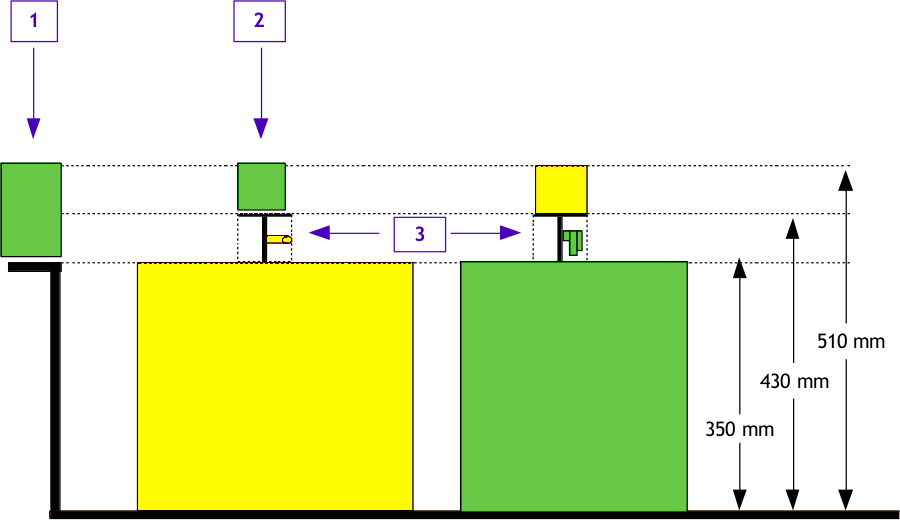
\includegraphics[height=.27\textheight]{balizas_robots}
\caption{Altura de balizas y sensores. Vista de perfil de dos robots oponentes y el campo de juego. 1- Soporte para balizas del campo de juego. 2- Soporte para baliza del oponente. 3- Espacio para sensores de balizas.}
\label{balizas_robots}
\end{figure}

\begin{figure}[ht]
\centering
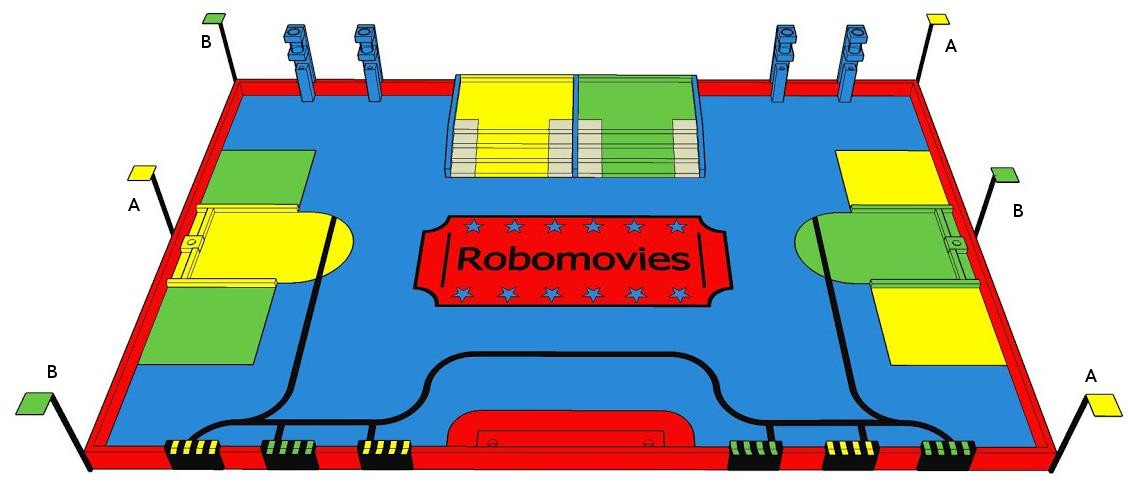
\includegraphics[height=.27\textheight]{balizas_campo}
\caption{Soportes para balizas del campo de juego. Campo de juego de Eurobot 2015. Soportes para balizas de los equipos A y B.}
\label{balizas_campo}
\end{figure}

Por otro lado, el robot ha de ser capaz de resolver la tem�tica del juego lo cual implica el manejo de los elementos o piezas propias del juego. Por ejemplo, en Eurobot 2015, juego titulado como Robomovies (tem�tica sobre el cine), una de las cosas por las que los robots obten�an puntos era por hacer una torre con piezas cil�ndricas coronada con una pelota de tenis que simbolizaba un foco de cine. 

Adem�s, mec�nicamente un robot ha de cumplir las siguientes restricciones dimensionales:

\begin{itemize}
\item Per�metro m�ximo inicial 1200 mm (700 mm para el robot secundario)
\item Per�metro m�ximo desplegado 1500 mm (900 mm para el robot secundario)
\item Altura m�xima de 350 mm
\end{itemize}


Por �ltimo, las reglas de Eurobot adem�s especifican otros temas que deben de ser tenidos en cuenta en caso de que apliquen:

\begin{itemize}
\item Fuentes de alimentaci�n y bater�as
\item Utilizaci�n de fuentes de luz y l�seres
\item Utilizaci�n de sistemas de comunicaci�n de radio
\item Utilizaci�n de sistemas de aire comprimido
\item Bot�n de parada de emergencia
\item M�todo de comienzo y finalizaci�n de un partido
\item Procedimientos de un partido.
\end{itemize}


\section{Partes principales en el desarrollo de un robot de Eurobot}

Teniendo en cuenta las especificaciones descritas en la secci�n anterior y la tem�tica de la prueba de Eurobot, el desarrollo de un robot de Eurobot se puede dividir en las siguientes partes principales:

\begin{enumerate}
\item Estrategia de juego.
\item Desplazamiento y localizaci�n.
\item Evitaci�n de obst�culos.
\item Comunicaci�n entre robots (en caso de jugar con 2 robots).
\item Manipulaci�n elementos de juego. 
\end{enumerate}

As�, tal y como representa la figura \ref{fig:partes_robot_eurobot}, un �nico robot est� compuesto por las tres primera partes y s�lo en caso de contar con 2 o m�s robots es necesaria la parte de comunicaci�n entre robots. 

\begin{figure}[h]
\centering
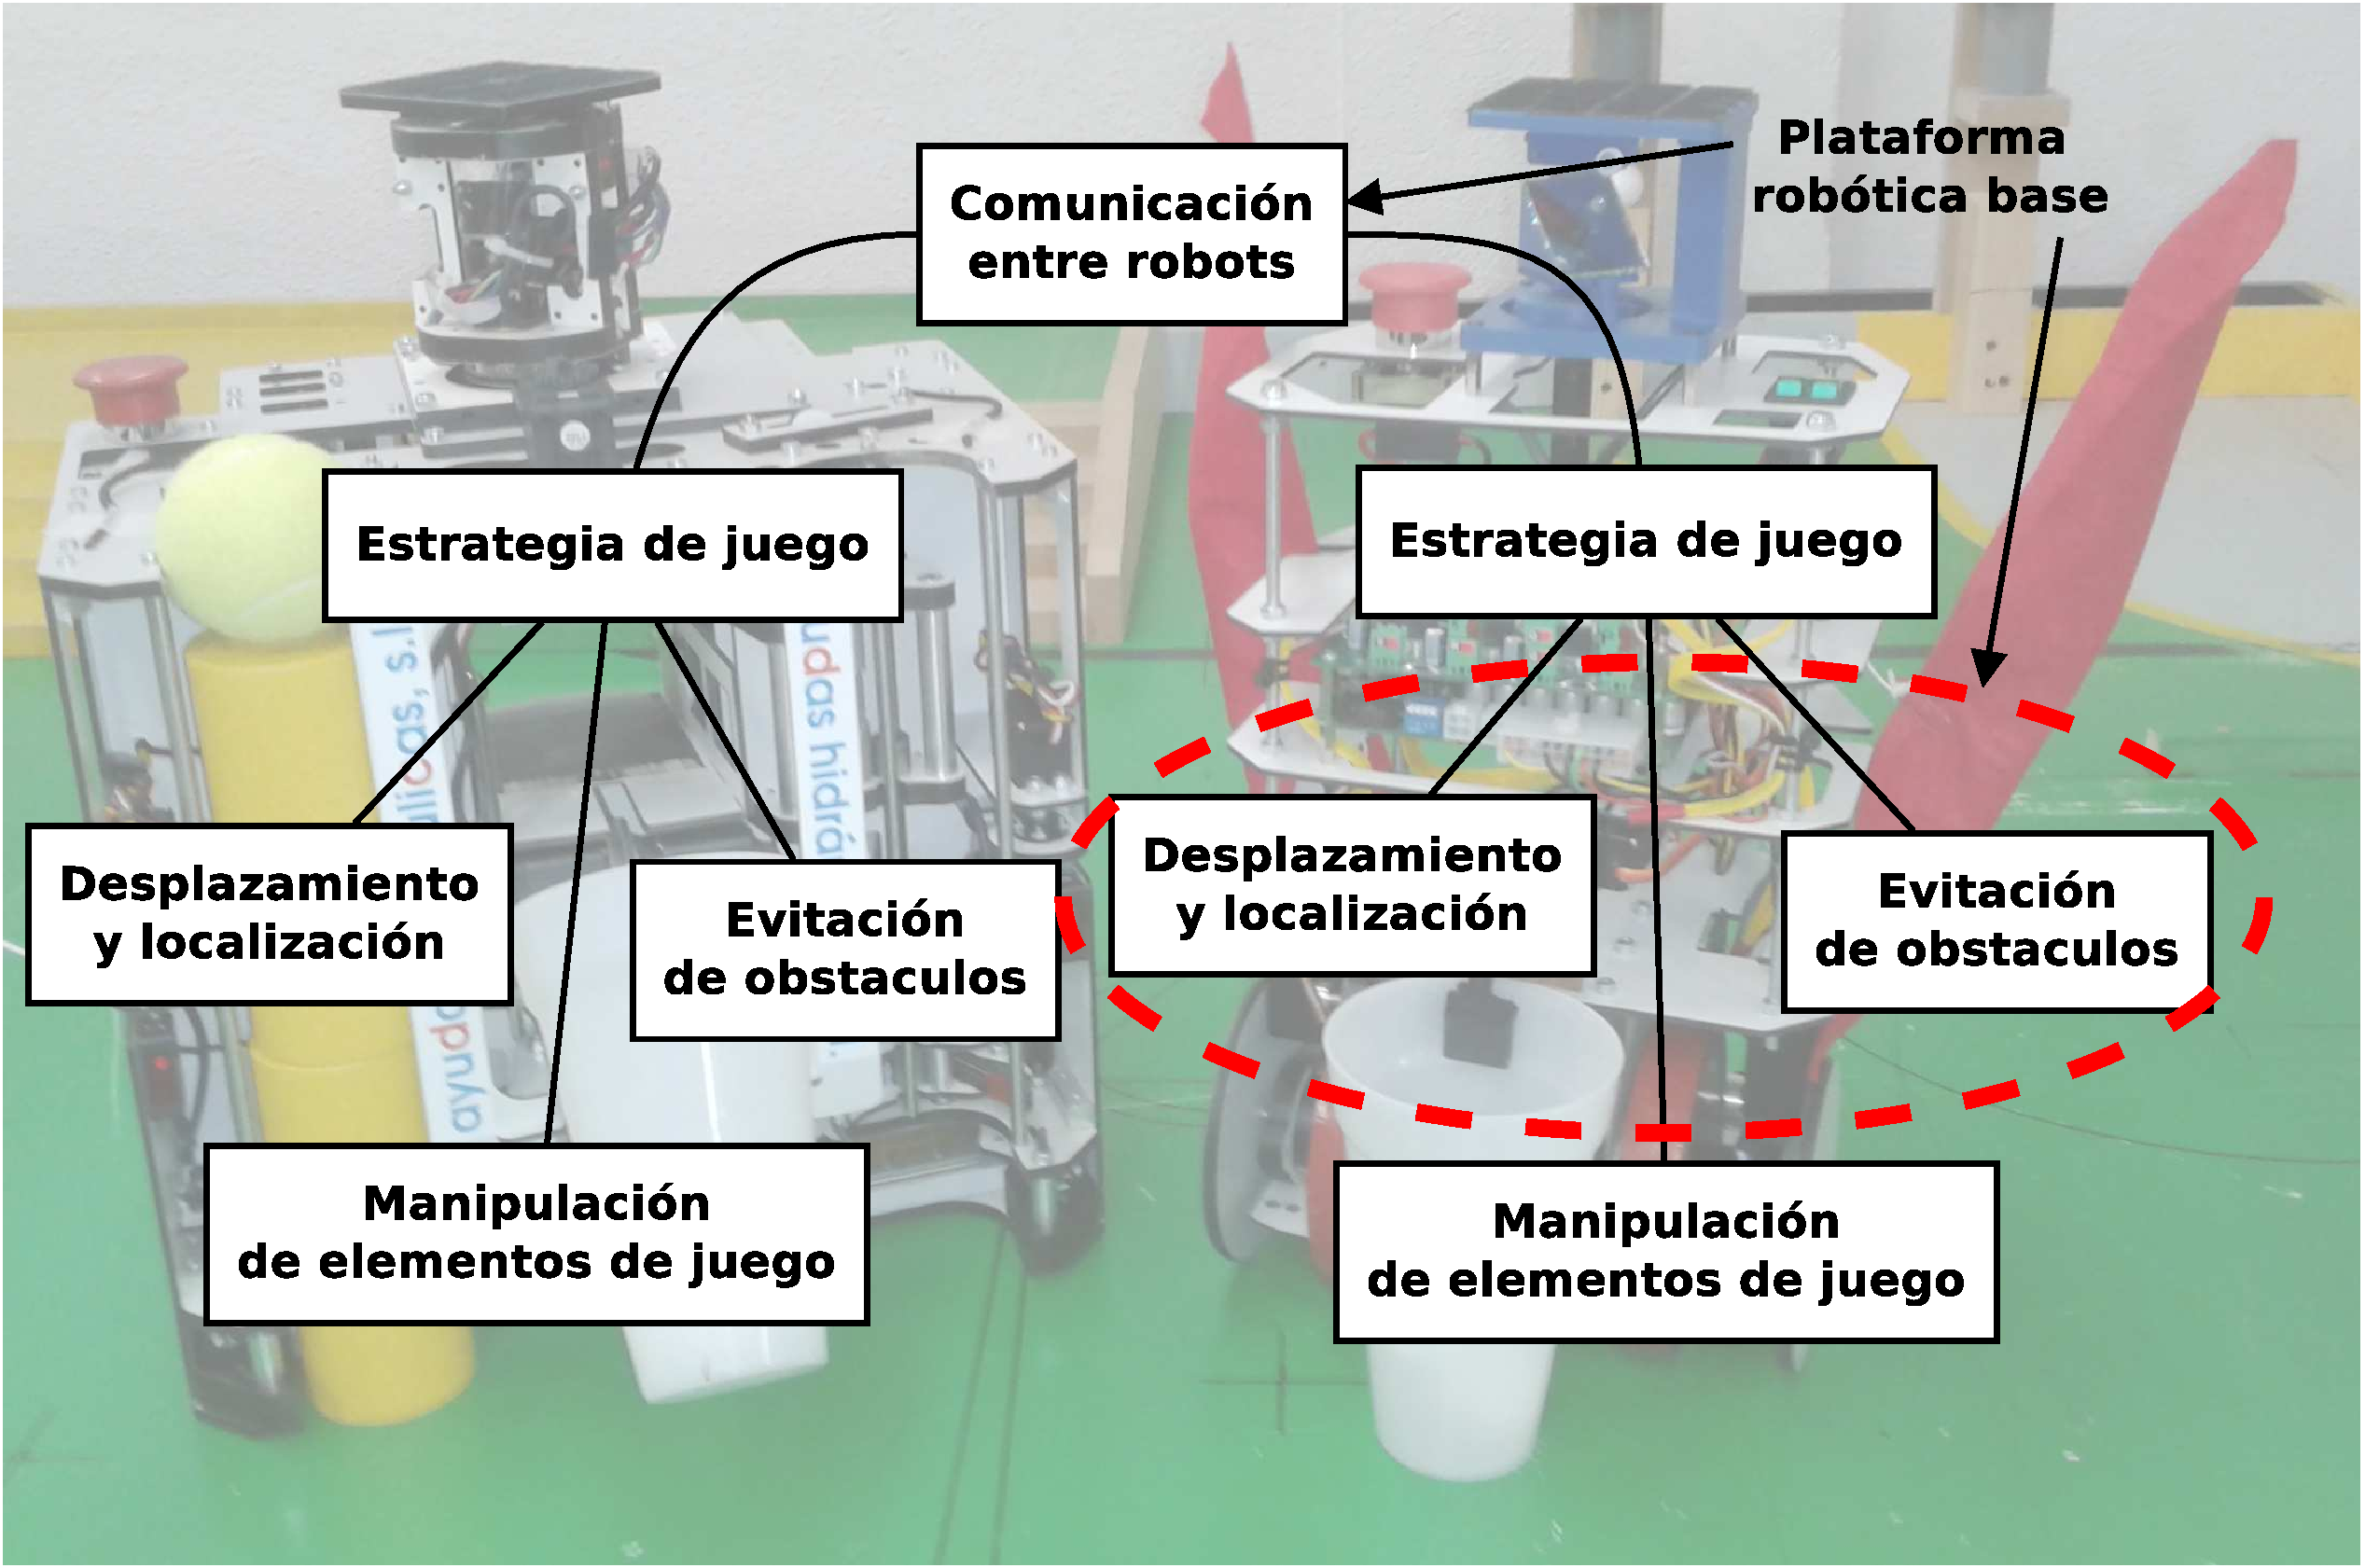
\includegraphics[height=.4\textheight]{partes_robot_eurobot}
\caption{Partes principales del desarrollo de un robot de Eurobot. En el fondo robot P.Tinto y Tirantes (robot secundario) desarrollados para Eurobot 2015 por el equipo Eurobotics Engineering}
\label{fig:partes_robot_eurobot}
\end{figure}

Por otro lado, las partes 2, 3 y 4 forman lo que se ha denominado \emph{plataforma rob�tica base}. Esta plataforma base est� compuesta por las partes que permiten un desarrollo independientemente de la tem�tica de la prueba de Eurobot. As�, esta plataforma rob�tica constituye un desarrollo reutilizable en la concepci�n de nuevos robots de Eurobot. 

Cada una de estas partes principales de un robot de Eurobot tienen pueden implicar un desarrollo mec�nico, electr�nico y de software, dependiendo el caso:

\begin{description}
\item Estrategia de juego.

La estrategia de juego constituye el nivel m�s abstracto del robot y tiene un desarrollo puramente software. La estrategia tiene en cuenta diferentes variables del juego (tareas por realizar, prioridad de tareas, posici�n del oponente, el tiempo transcurrido de partido, etc.) para tomar decisiones que maximicen la puntuaci�n a conseguir y as� ganar el partido.

El desarrollo de la estrategia puede ser realizado en paralelo a otras partes del robot, pero ha de tener en cuenta los tiempos derivados de tareas que impliquen sistemas mec�nicos, como por ejemplo coger una pelota y almacenarla o desplazarse de un punto del campo a otro. Dichos tiempos por lo general son mucho mayores (segundos o decenas de segundos) que el tiempo que tarda el algoritmo de estrategia implementado en tomar una decisi�n. Es por ello que dicho algoritmo estar� la mayor parte del tiempo esperando a que otras partes terminen de realizar su funci�n.

\item Desplazamiento y localizaci�n.

El desplazamiento y localizaci�n del robot de Eurobot implica un desarrollo conjunto de mec�nica, electr�nica y software. 

El desplazamiento lleva impl�cito una localizaci�n, ambas funciones permiten realizar trayectorias desde un punto de inicio hasta un punto de destino y con una velocidad y aceleraci�n determinadas.   

\item Evitaci�n de obst�culos.
\item Comunicaci�n entre robots (en caso de jugar con 2 robots).
\item Manipulaci�n elementos de juego. 

\end{description}

\section{Arquitecturas mec�nica, hardware y software}

\section{Fases y metodolog�a de dise�o}

\begin{itemize}
\item Enfoque del proyecto y los esfuerzos: desarrollar un robot vs. desarrollar un sensor.
\item Desde la inexperiencia
\item Grano fino / grano grueso
\item Grano grueso puede limitar el dise�o mec�nico
\end{itemize}

\section{Depuraci�n y puesta en marcha}



%%% Local Variables:
%%% TeX-master: "../book"
%%% End:


%\chapter{El equipo de Eurobot}
%\section{Introducci�n}
%\section{Numero de integrantes}
%\section{Expectativas, motivaci�n y objetivos}
%\section{Tareas principales}
%\section{Organizaci�n y metodolog�a del trabajo}

%%%%%%%%%%%%%%%%%%%%%%%%%%%%%%%%%%%%%%%%%%%%%%%%%%%%%%%%%%%%%%%%%%%%%%%%%%%
%
% Generic template for TFC/TFM/TFG/Tesis
%
% $Id: introduccion.tex,v 1.6 2014/02/11 11:00:06 macias Exp $
%
% By:
%  + Javier Mac�as-Guarasa.
%    Departamento de Electr�nica
%    Universidad de Alcal�
%  + Roberto Barra-Chicote.
%    Departamento de Ingenier�a Electr�nica
%    Universidad Polit�cnica de Madrid
%
% Based on original sources by Roberto Barra, Manuel Oca�a, Jes�s Nuevo,
% Pedro Revenga, Fernando Herr�nz and Noelia Hern�ndez. Thanks a lot to
% all of them, and to the many anonymous contributors found (thanks to
% google) that provided help in setting all this up.
%
% See also the additionalContributors.txt file to check the name of
% additional contributors to this work.
%
% If you think you can add pieces of relevant/useful examples,
% improvements, please contact us at (macias@depeca.uah.es)
%
% Copyleft 2013
%
%%%%%%%%%%%%%%%%%%%%%%%%%%%%%%%%%%%%%%%%%%%%%%%%%%%%%%%%%%%%%%%%%%%%%%%%%%%

\chapter{Plataforma rob�tica base}
\label{cha_plataforma_robotica_base}

\begin{FraseCelebre}
  \begin{Frase}
La imaginaci�n es m�s importante que el conocimiento. El conocimiento es limitado y la imaginaci�n circunda el mundo.    
  \end{Frase}
  \begin{Fuente}
Albert Einstein, en \emph{The Saturday Evening Post}
  \end{Fuente}
\end{FraseCelebre}


%\section{Introducci�n}

En el a�o 2010 se desarroll� una plataforma rob�tica base, cuyo dise�o fue reutilizado y mejorado en el desarrollo de robots posteriores. Dicha plataforma incluye las funcionalidades b�sicas de un robot de Eurobot vistas en el capitulo \ref{cha_el_robot_de_eurobot}:

\begin{itemize}
\item Desplazamiento y localizaci�n
\item Evitaci�n de obst�culos
\item Comunicaci�n entre robots
\end{itemize}

El desarrollo de cada una de estas funcionalidades constituye en s� una la labor de ingenier�a muy interesante que implica la aplicaci�n de fundamentos de diferentes campos de la ciencia y la ingenier�a. 

\section{Descripci�n general de la plataforma rob�tica}

La funci�n de \textbf{desplazamiento y localizaci�n} de la plataforma rob�tica se implementa a partir de un \emph{sistema de tracci�n diferencial} y un \emph{sistema de posicionamiento por odometr�a}. Mediante la uni�n de estos dos sistemas implementa a su vez un \emph{control de posici�n polar}, a partir del cual, se gestiona la \emph{generaci�n de trayectorias}.

Mec�nicamente el sistema de tracci�n diferencial consiste en un bloque motor formado por dos motores unidos mediante una reductora mec�nica a dos ruedas motrices (ver figura \ref{fig_plataforma_partes_1}). Sobre el eje motriz, en sus extremos, el robot tiene dos ruedas libres conectadas a sensores tipo encoder que se utilizan para implementar el sistema de posicionamiento por odometr�a y, junto con el bloque motor, el control de posici�n del robot.

\begin{figure}[ht]
\centering
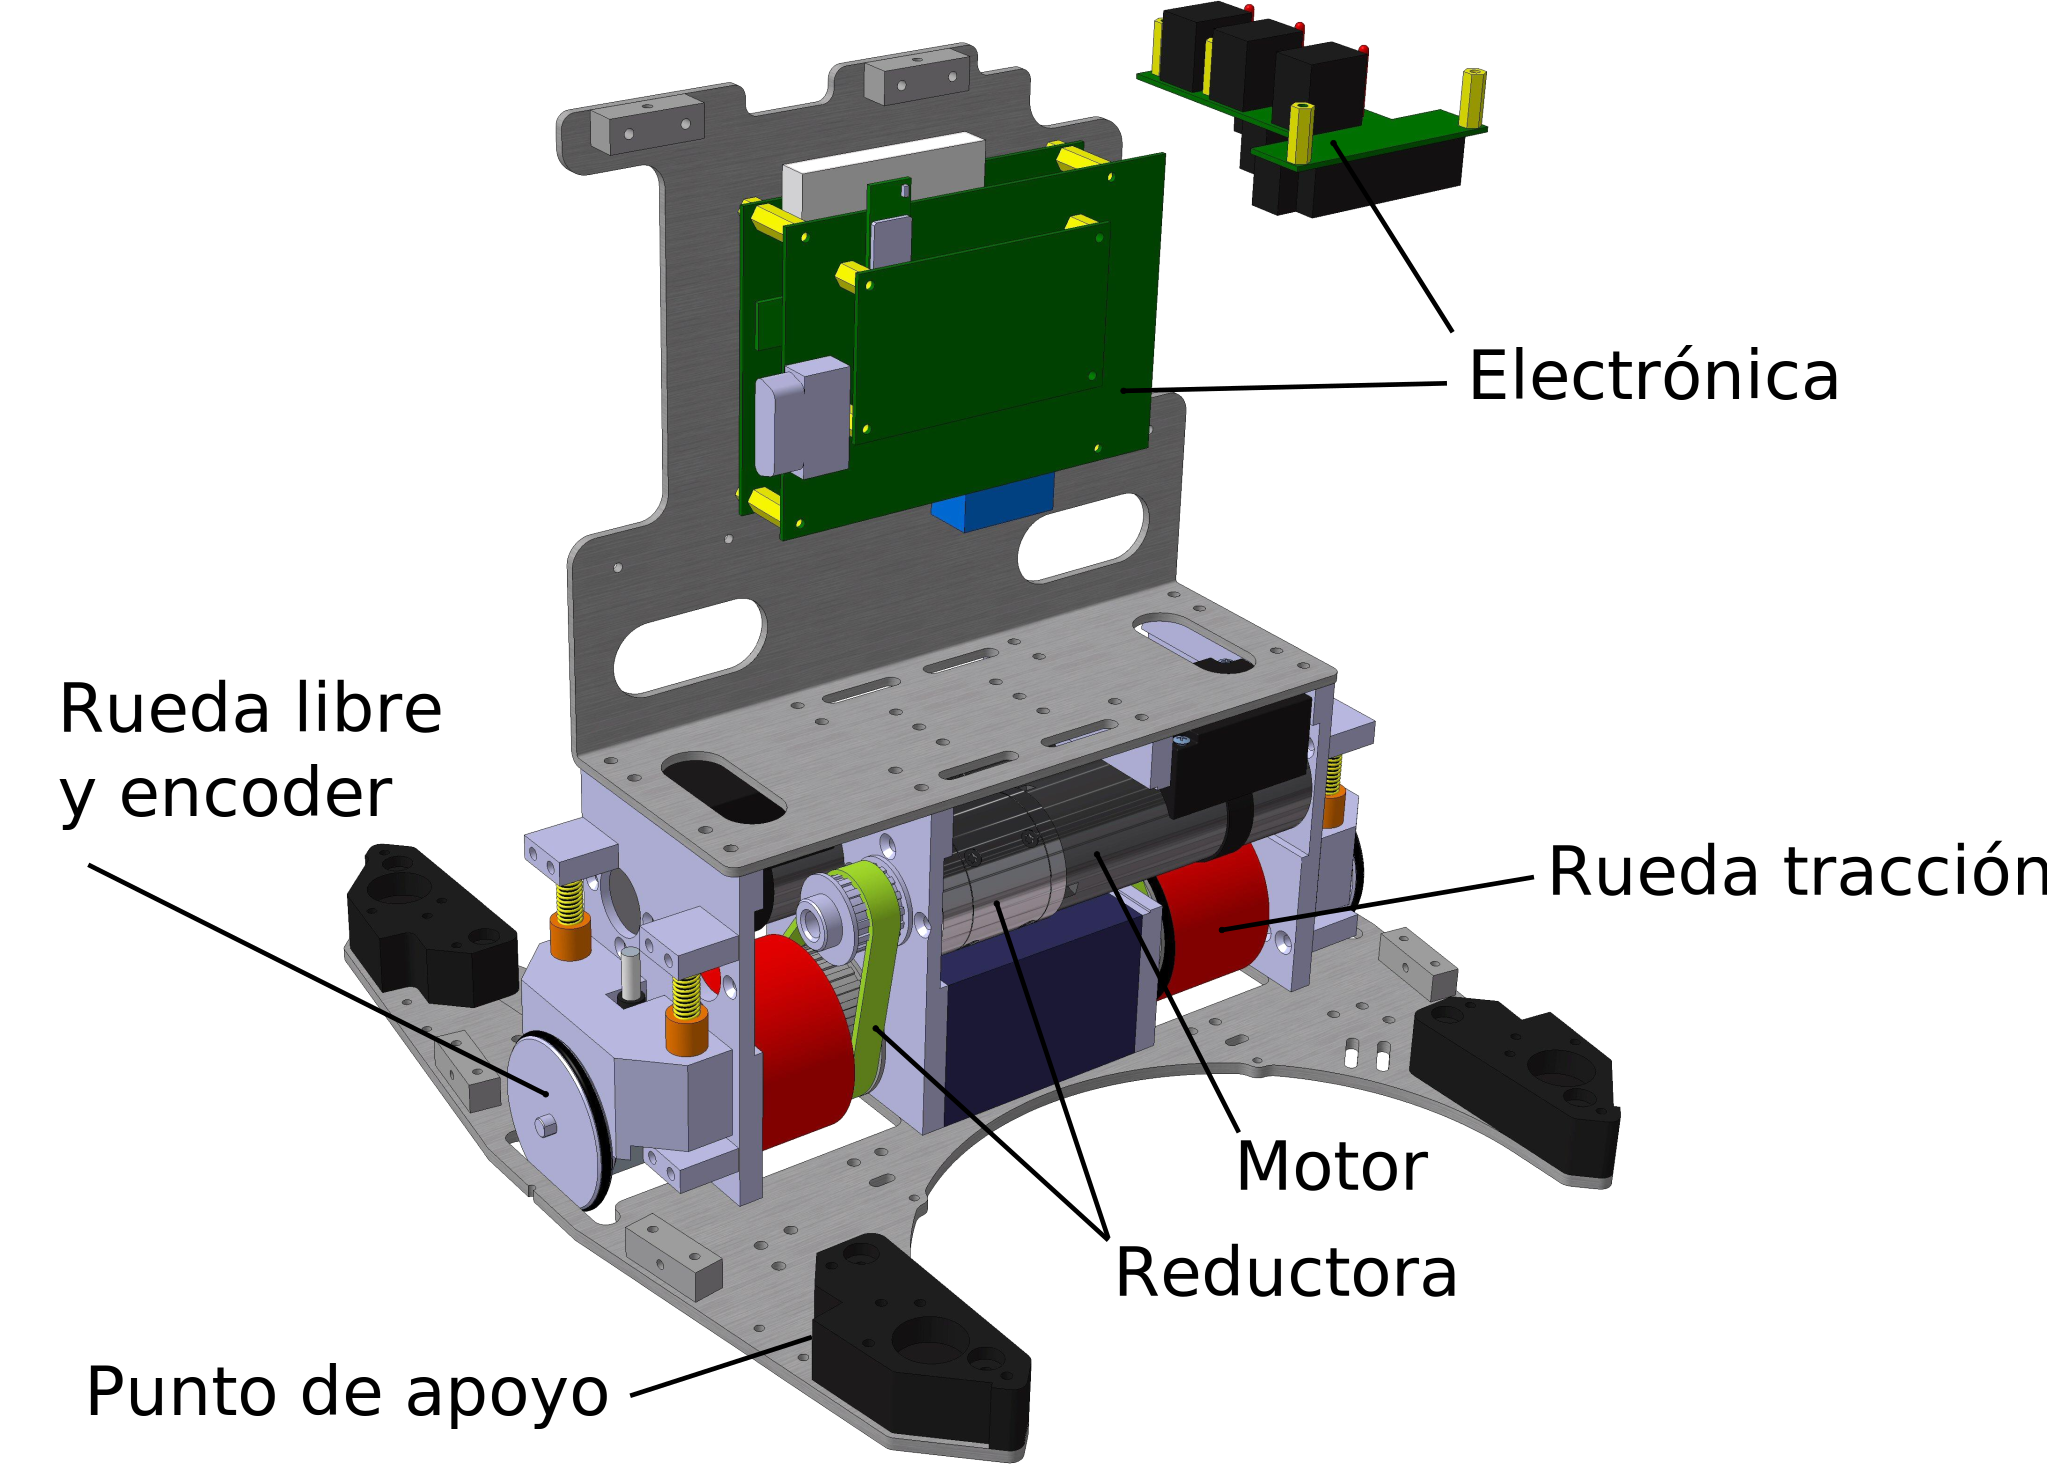
\includegraphics[height=.3\textheight]{plataforma_partes_1}
\caption[Plataforma rob�tica base: partes del sistema de tracci�n diferencial y del sistema de control de posici�n]{Plataforma rob�tica base: partes del sistema de tracci�n diferencial y del sistema de control de posici�n. Robot Zamorano (Eurobot 2011).}
\label{fig_plataforma_partes_1}
\end{figure}

El \textbf{hardware desarrollado} de la plataforma rob�tica est� compuesto por una tarjeta principal y varias tarjetas auxiliares que en conjunto tienen la capacidad de gestionar e implementar los sistemas mencionados anteriormente, as� como los sistemas mec�nicos espec�ficos de la prueba de Eurobot, destinados a la manipulaci�n de elementos de juego.

Respecto a la \textbf{evitaci�n de obst�culos}, esta se realiza a partir de sensores de distancia situados en las caras del robot (ver figura \ref{fig_plataforma_partes_2}) y a partir un sistema de balizas espec�ficamente desarrollado para la medida de la posici�n del oponente. Este sistema hace uso de los soportes y espacios destinados a sistemas de balizas. Concretamente, el sistema desarrollado est� basado en un sensor tipo faro situado en el robot y balizas reflectantes situadas en el oponente (ver figura \ref{fig_plataforma_partes_2}). El sistema de balizas es totalmente aut�nomo y se comunica mediante \emph{Bluetooth} con la tarjeta principal la plataforma rob�tica.

\begin{figure}[ht]
\centering
\includegraphics[height=.3\textheight]{plataforma_partes_2}
\caption[Plataforma rob�tica base: partes del sistema de evitaci�n de obst�culos]{Plataforma rob�tica base: partes del sistema de evitaci�n de obst�culos. Robot Zamorano (Eurobot 2011).}
\label{fig_plataforma_partes_2}
\end{figure}

La \textbf{implementaci�n software} de todos los sistemas y funcionalidades de la plataforma rob�tica ha sido realizada a partir de las librer�as Aversive4dspic. Estas librer�as han sido migradas de las librer�as Aversive \cite{aversive_src}, desarrolladas para microcontroladores AVR, a microcontroladores dsPIC (utilizados por la tarjeta principal de la plataforma robot). Entre las caracter�sticas de las librer�as Aversive y Aversive4dspic se encuentran modulos espec�ficos para la implementaci�n de sistemas de control y de robots como los de Eurobot.

Por �ltimo, la plataforma rob�tica desarrollada permite que en caso de contar con \textbf{dos robots por equipo}, la misma  arquitectura mec�nica, hardware y software pueda ser utilizada en el robot principal y secundario. Y la comunicaci�n entre ambos robots puede ser implementada mediante la inferfaz \emph{Bluetooth} de las tarjetas principales de cada robot.


\section{Sistema de tracci�n diferencial}
\label{sec_sistema_traccion_diferencial}
El sistema de tracci�n diferencial es uno de los m�s comunes en Eurobot, est� compuesto por dos ruedas motrices unidas a motores mediante una reductora y varios puntos de apoyo (ver figura \ref{fig_plataforma_partes_1}). 

Dependiendo de la posici�n del eje motriz se dan 2 tipos de robots:

\begin{enumerate}
\item Robot con ruedas atr�s: necesitan de dos puntos de apoyo delanteros.
\item Robot con ruedas en el medio: necesitan de puntos de apoyo delanteros y traseros.
\end{enumerate}

Los robots con ruedas atr�s suelen tener dos puntos de apoyo delanteros. En cambio, los robots con ruedas en el medio suelen tener dos puntos de apoyo delanteros y otros dos traseros. Aunque a veces en uno de los extremos s�lo llevan un punto de apoyo, 3 puntos de apoyo en total.

Como se ver� m�s adelante, interesa un robot con ruedas en el medio y que tenga una simetr�a total de forma que todo el peso del robot recaiga sobre el eje motriz. Adem�s, los puntos de apoyo han de estar a la mayor distancia posible del eje motriz. Esta situaci�n no siempre se cumple, ya que existe un compromiso con el resto de elementos mec�nicos del robot.

Los puntos de apoyo utilizados normalmente son de tipo \emph{rollon}. En caso de no disponer de espacio suficiente para ellos tambi�n es posible utilizar materiales de bajo coeficiente de rozamiento como el tefl�n (ver figura \ref{fig_sistema_traccion_rollones}).

\begin{figure}[ht]
\centering
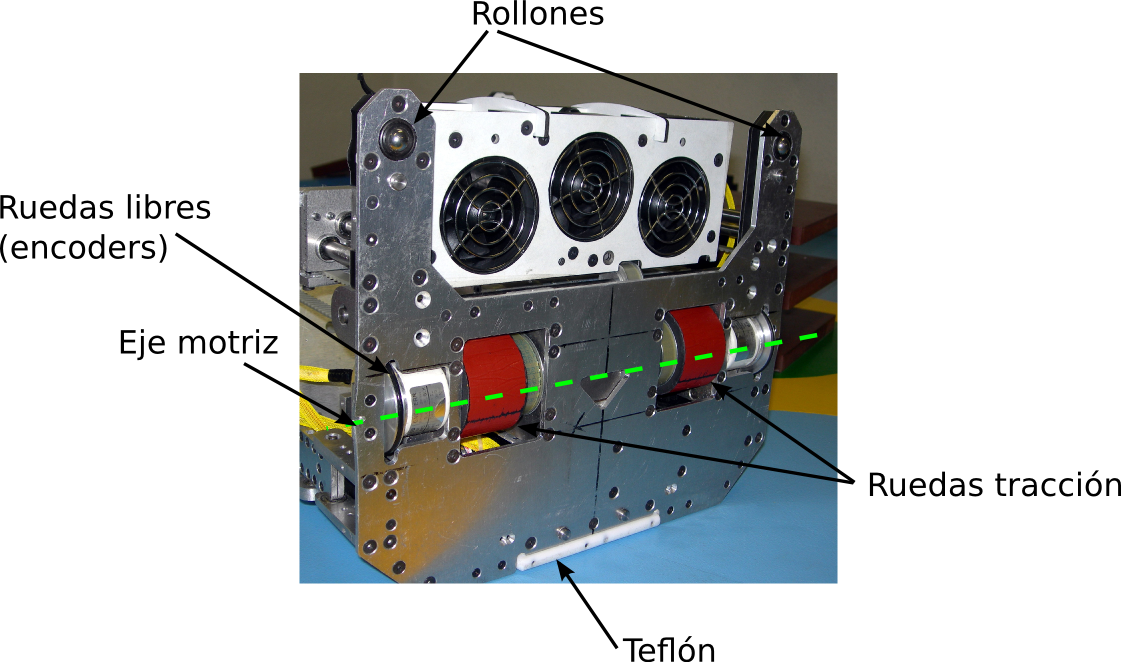
\includegraphics[height=.3\textheight]{sistema_traccion_rollones}
\caption[]{Sistema de tracci�n diferencial del robot Autom�tico (Eurobot 2013) visto desde abajo.}
\label{fig_sistema_traccion_rollones}
\end{figure}

Mec�nicamente el conjunto de los motores, reductora y ruedas se denomina \emph{bloque motor}. El bloque motor se reutiliza como una parte independiente en cada dise�o de un nuevo robot de forma que se sit�a sobre la base del robot adapt�ndose al resto de la mec�nica.


\section{Sistema de posicionamiento y control de posici�n}
\label{sec_sma_posicionamiento_y_control}

La medida de la posici�n del robot se realiza mediante dos ruedas libres unidas a sensores tipo encoders. A partir de dicha medida de posici�n se implementa indirectamente el control de posici�n de los motores del sistema de tracci�n y de forma directa el sistema de posicionamiento por odometr�a del robot. Esta configuraci�n difiere del esquema cl�sico en el que el encoder se encuentra conectado directamente al eje del motor, permite reducir los errores sistem�ticos de odometr�a \cite{bor96_cap5} y que un posible deslizamiento o derrape de las ruedas motrices no afecte al control de posici�n del robot.

Es posible que adem�s los motores tengan un encoder conectado directamente su eje de forma que se implemente un doble lazo de control: un control de posici�n o velocidad de los motores y un control de posici�n del robot. Sin embargo, el uso de encoders incrementales de al menos 2000 pulsos por vuelta en las ruedas libres y el hecho de que el robot siempre est� en contacto con el suelo, hace que los encoders de los motores resultar�an redundantes e incrementen el procesado software y los recursos necesarios del hardware.


\begin{figure}[ht]
\centering
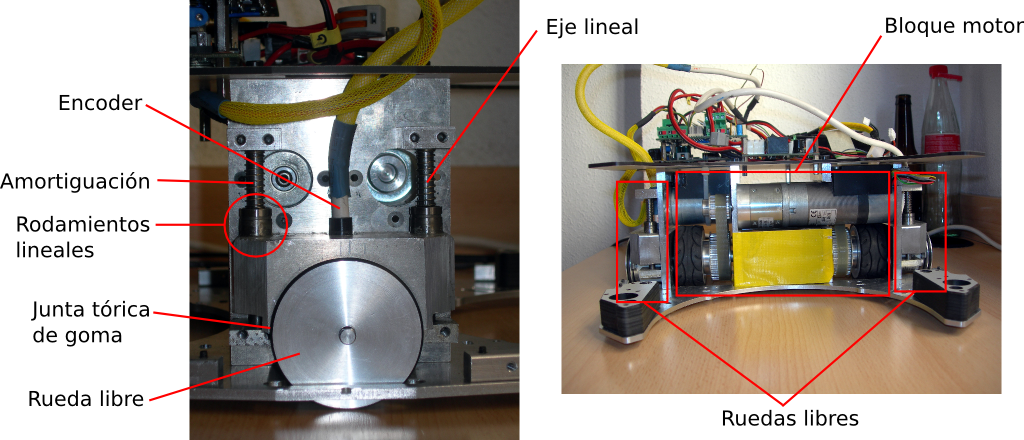
\includegraphics[width=.9\textwidth]{ruedas_libres_lineal}
\caption[]{Sistema de ruedas libres lineal}
\label{fig_ruedas_libres_lineal}
\end{figure}

Inicialmente, para el robot Trompetero (Eurobot 2010) se implemento un sistema de ruedas libres lineal como el de la figura \ref{fig_ruedas_libres_lineal}. Este sistema esta compuesto por una rueda que como neum�tico tiene una junta t�rica de goma. Dicha rueda se encuentra conectada con un encoder incremental de dos canales en cuadratura. El conjunto rueda y encoder se encuentran fijados a la base del robot mediante un sistema de dos gu�as lineales con amortiguaci�n. La amortiguaci�n permite asegurar que ante cualquier desperfecto del campo la rueda siempre est� en contacto con el suelo. Cada guia tiene dos rodamientos lineales para disminuir el rozamiento. La implementaci�n de este sistema mec�nico es complejo y necesita de un ajuste de cierta precisi�n de forma que las dos gu�as lineales se encuentre perfectamente paralelas para que no existan rozamientos que impliquen errores no sistem�ticos.

\begin{figure}[ht]
\centering
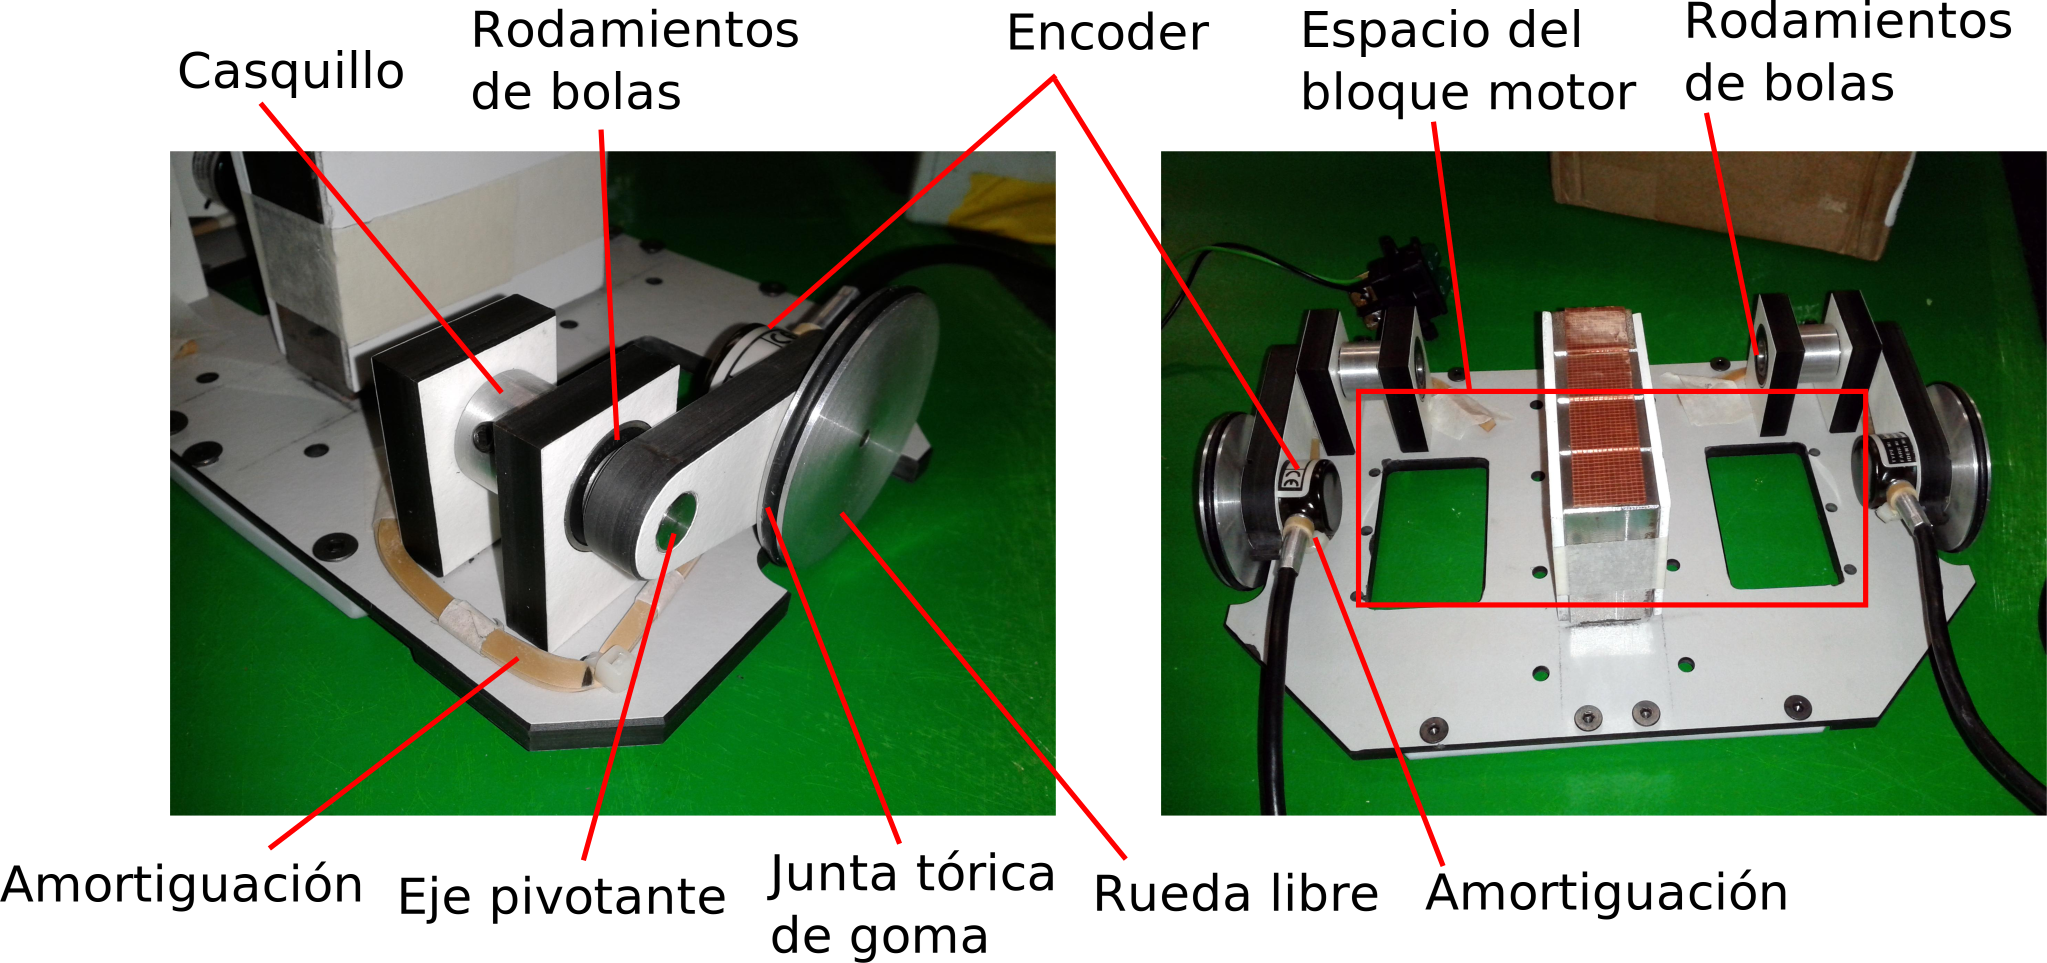
\includegraphics[width=.9\textwidth]{ruedas_libres_pivotante}
\caption[]{Sistema de ruedas libres pivotante}
\label{fig_ruedas_libres_pivotante}
\end{figure}

Un sistema mec�nico m�s sencillo tanto en implementaci�n y como en ajuste es el sistema de ruedas libres pivotante (ver figura \ref{fig_ruedas_libres_pivotante}). Este sistema fue implementado por primera vez en el robot secundario Seskapa (Eurobot 2014) dado el poco espacio disponible y posteriormente en los robots P.Tinto y Tirantes (Eurobot 2015). En este sistema, el conjunto rueda y encoder pivotan sobre un eje paralelo al eje motriz. Dicho eje se encuentra fijado a la base del robot mediante dos piezas con rodamientos de bolas separadas por un casquillo que evita que el eje se desplace. Este sistema tiene menos puntos de ajuste que el sistema lineal. Adem�s la amortiguaci�n del sistema es casi innecesaria debido al bajo rozamiento del eje con los rodamientos de bolas. El propio peso del conjunto rueda y encoder garantiza el contacto con el suelo. No obstante como se ve en la figura \ref{fig_ruedas_libres_pivotante} se utiliz� unas gomas el�sticas para asegurar el contacto con el suelo. El inconveniente de este sistema se debe al propio pivote, si el suelo tiene muchas imperfecciones, al pivotar la rueda esta se desalinea respecto al eje motriz, lo cual puede generar errores de medida de posici�n. Este echo es despreciable frente a la simplicidad de implementaci�n mec�nica y a que el suelo del campo de juego es plano.


\section{Estudio de la din�mica de robots de tracci�n diferencial}

El estudio de la din�mica de un robot de tracci�n diferencia permite conocer los l�mites de aceleraci�n y velocidad a partir de los cuales dimensionar la reductora y los motores que mueven el robot.

En las siguientes secciones se analizar la din�mica de un robot de tracci�n diferencia en desplazamientos lineales sobre el plano horizontales. El modelo din�mico para este caso es sencillo y permite deducir restricciones mec�nica muy �tiles a la hora de dise�ar un robot de estas caracter�sticas.

No es objeto de este proyecto analizar el modelo din�mico del robot para desplazamientos angulares. El c�lculo de dicho modelo resulta muy complejo comparado con la influencia de estos movimientos en un robot de Eurobot. Es en los desplazamientos lineales donde el robot ha de adaptar su velocidad y aceleraci�n para evitar chocar con el oponente o alcanzar una posici�n del campo.

\subsection{Din�mica b�sica en desplazamientos lineales sobre un plano horizontal}

Es importante entender la din�mica de un robot de Eurobot y tenerla en cuenta durante el dise�o mec�nico del mismo. El movimiento m�s com�n de un robot de Eurobot son los desplazamientos entre dos puntos. Durante dichos desplazamientos el robot parte de parado, recorre una distancia y vuelve a detenerse. As�, a cada desplazamiento le corresponde una fase de aceleraci�n, una fase de velocidad constante y otra fase de frenado.

Para el caso de un robot con ruedas atr�s y dos puntos de apoyo, el modelo din�mico del robot, seg�n describe el equipo RCVA en \cite{rcva_10x}, queda representado por la figura siguiente:

\begin{figure}[H]
\centering
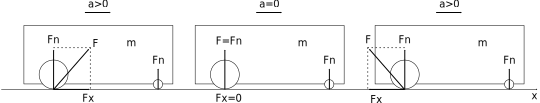
\includegraphics[width=\textwidth]{dinamica_basica}
\caption[Modelo din�mico simple de un robot de tracci�n diferencial]{Modelo din�mico simple de un robot de tracci�n diferencial.}
\label{fig_dinamica_basica}
\end{figure}

Siendo:
\begin{description}
\item $F_n$: fuerza normal o vertical del suelo (opuesta a la fuerza de apoyo debida al peso del robot)
\item $F_x$: fuerza de propulsi�n de en la rueda
\item $F$: fuerza resultante del suelo en la rueda
\item $a$: aceleraci�n del robot
\item $m$: masa del robot sobre las ruedas.
\end{description}

Durante la fase de aceleraci�n ($a>0$) se necesita una fuerza de propulsi�n $F_x$ positiva de forma que la fuerza resultante $F$ provoque un desplazamiento hacia delante. Una vez alcanzada la fase de velocidad constante ($a=0$), te�ricamente no es necesario realizar ninguna fuerza de propulsi�n\footnote{En la pr�ctica, dado que existen perdidas por rozamiento $F_x$ no es nula. Aun as� la fuerza para mantener una velocidad constante es menor que la necesaria para acelerar el robot hasta esa velocidad. El efecto es el mismo experimentado al mover un armario, una vez vencida la fuerza de rozamiento inicial la fuerza necesaria para desplazarlo es m�nima.} y la fuerza resultante es igual a la fuerza normal sobre la rueda. En la �ltima fase, la fuerza de tracci�n $F_x$ ha de ser negativa de forma que la fuerza resultante se oponga al movimiento del robot provocando una desaceleraci�n o frenado.  

Para conseguir desplazamientos en un periodo de tiempo corto, las fases de aceleraci�n y frenado han de durar lo menos posible. El valor de la aceleraci�n durante esas fases va a depender por un lado del coeficiente de adherencia de las ruedas, y por otro, de la posici�n del centro de gravedad del robot.


\subsection{Coeficiente de adherencia de las ruedas y su c�lculo experimental}
\label{coeficiente_adherencia_y_calculo_experimental}

A partir del modelo din�mico descrito anteriormente, teniendo en cuenta que el robot dispone de dos ruedas (un motor por rueda) y a partir de la primera ley de Newton ($F = ma$) se deduce que la aceleraci�n sobre el eje horizontal del robot se corresponde con la expresi�n:
\begin{equation}
  \label{eq_a_f_fx}
  a = \frac{2F_x}{m}
\end{equation}


La aceleraci�n m�xima vendr� dada por la fuerza m�xima de propulsi�n de las ruedas $F_{x\,max}$ a partir de la cual se produce el deslizamiento de las ruedas. Por lo tanto ha de cumplirse la condici�n
\begin{equation}
  \label{eq_condicion_fx}
   F_x<F_{x\,max}
\end{equation}

siendo
\begin{equation}
  \label{eq_fx_max_f_ka}
  F_{x\,max} = K_a \, F_n,
\end{equation}

donde $K_a$ es el coeficiente de adherencia de las ruedas contra el suelo y toma valores te�ricos ente 0 y 1:

$K_a=0$: adherencia nula

$K_a=1$: adherencia te�rica m�xima\footnote{En la practica el coeficiente de adherencia puede superar valores de uno, por ejemplo si existe una carga aerodin�mica extra como ocurre en los coches de carreras de la F1.}.

El valor de $K_a$ depende del tipo de neum�tico utilizado y de la calidad y limpieza del campo de juego. As� para un neum�tico consistente en una junta t�rica se consiguen valores de $K_a$ inferiores a $0,5$. En cambio un neum�tico de caucho de baja dureza (entre 20 y 30 shores) podr�a alcanzar valores de $K_a$ cercanos a 1. 

%El coeficiente de adherencia permite calcular, junto con la posici�n del centro de gravedad del robot, la aceleraci�n m�xima del mismo. 
El valor del coeficiente de adherencia se puede medir experimentalmente mediante el m�todo propuesto por Jacques Coulon en \cite{rcva_10x}, conocido como el \emph{m�todo del cubo}. 

\begin{figure}[ht]
\centering
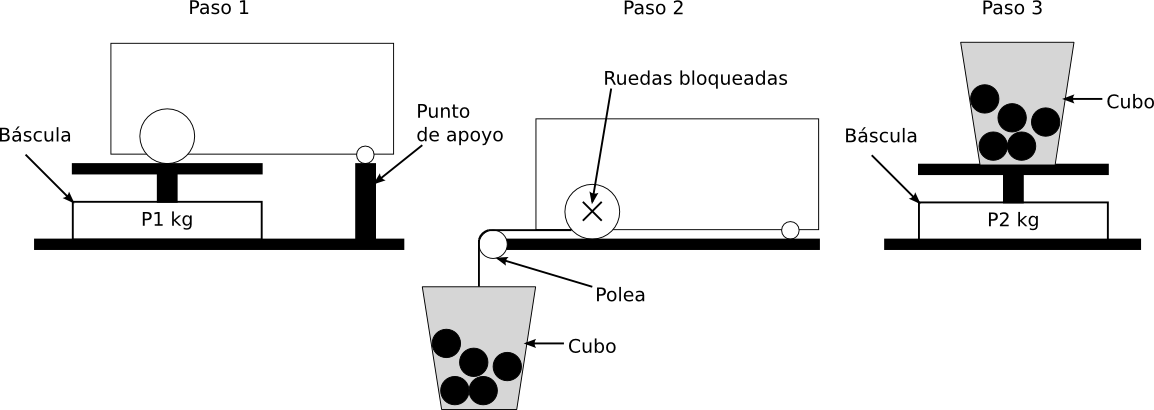
\includegraphics[width=\textwidth]{metodo_cubo}
\caption[]{Medodo de medida del coeficiente de adherencia de las ruedas.}
\label{fig_metodo_cubo}
\end{figure}


Dicho m�todo se encuentra representado en la figura \ref{fig_metodo_cubo} y consta de tres pasos:

\begin{enumerate}
\item Apoyar las ruedas del robot sobre una b�scula manteniendo el robot horizontal. Para ello, ayudarse de un soporte sobre los puntos de apoyo del robot. El peso $P1$ medido por la bascula se corresponde con la fuerza con la que las ruedas apoyan en el suelo.
\item Bloquear las ruedas del robot\footnote{El boqueo ha de ser un bloqueo mec�nico, en caso de bloquear las ruedas manteniendo la consigna de posici�n del robot el motor puede resultar gravemente da�ado.} y fijar a la parte m�s baja y cercana al eje motriz una cuerda atada a un cubo. Hacer pasar la cuerda por una polea para disminuir el rozamiento y a�adir peso al cubo hasta que las ruedas comiencen a deslizar.
\item Medir el peso $P2$ del cubo, el cual se corresponde con la fuerza de tracci�n m�xima en el l�mite de deslizamiento.
\end{enumerate}

El coeficiente de adherencia viene dado por las medidas realizadas seg�n la expresi�n
\begin{equation}
  \label{eq_ka=f(p1,p2)}
  \boxed{K_a = \frac{P2}{P1}}.
\end{equation}

Notar que el valor de $K_a$ es independiente del peso del robot.

La validez de este m�todo se ha comprobado en la practica. El m�todo se aplic� a robots de diferente peso y de ruedas id�nticas obteniendo los resultados de la tabla siguiente:


\begin{table}[ht]
\centering
\caption{Resultados de la medida del coeficiente de adherencia de las ruedas}
\label{tab_resultados_medida_ka}
\begin{tabular}{lccc}
\hline
Robot & $P1$ & $P2$ & $K_a$ \\
\hline
Zamorano (2011) 	& 14,5   & 15,6   & 1,076  \\
Autom�tico (2012)   & 17,6   & 17,3   & 0,983  \\
\hline
\end{tabular}
\end{table}

Las ruedas de ambos robots se muestra en la figura \ref{fig_ruedas_foam_silicona}. Est�n construidas a partir de ruedas de coche de radio control de espuma, 60mm de di�metro y 45mm de ancho. Adem�s se les ha a�adido una capa de silicona para mejorar la adherencia. Este tipo de ruedas ha sido utilizado en todos los robots desarrollados desde el a�o 2011 dado su alto coeficiente de adherencia. 

\begin{figure}[h]
\centering
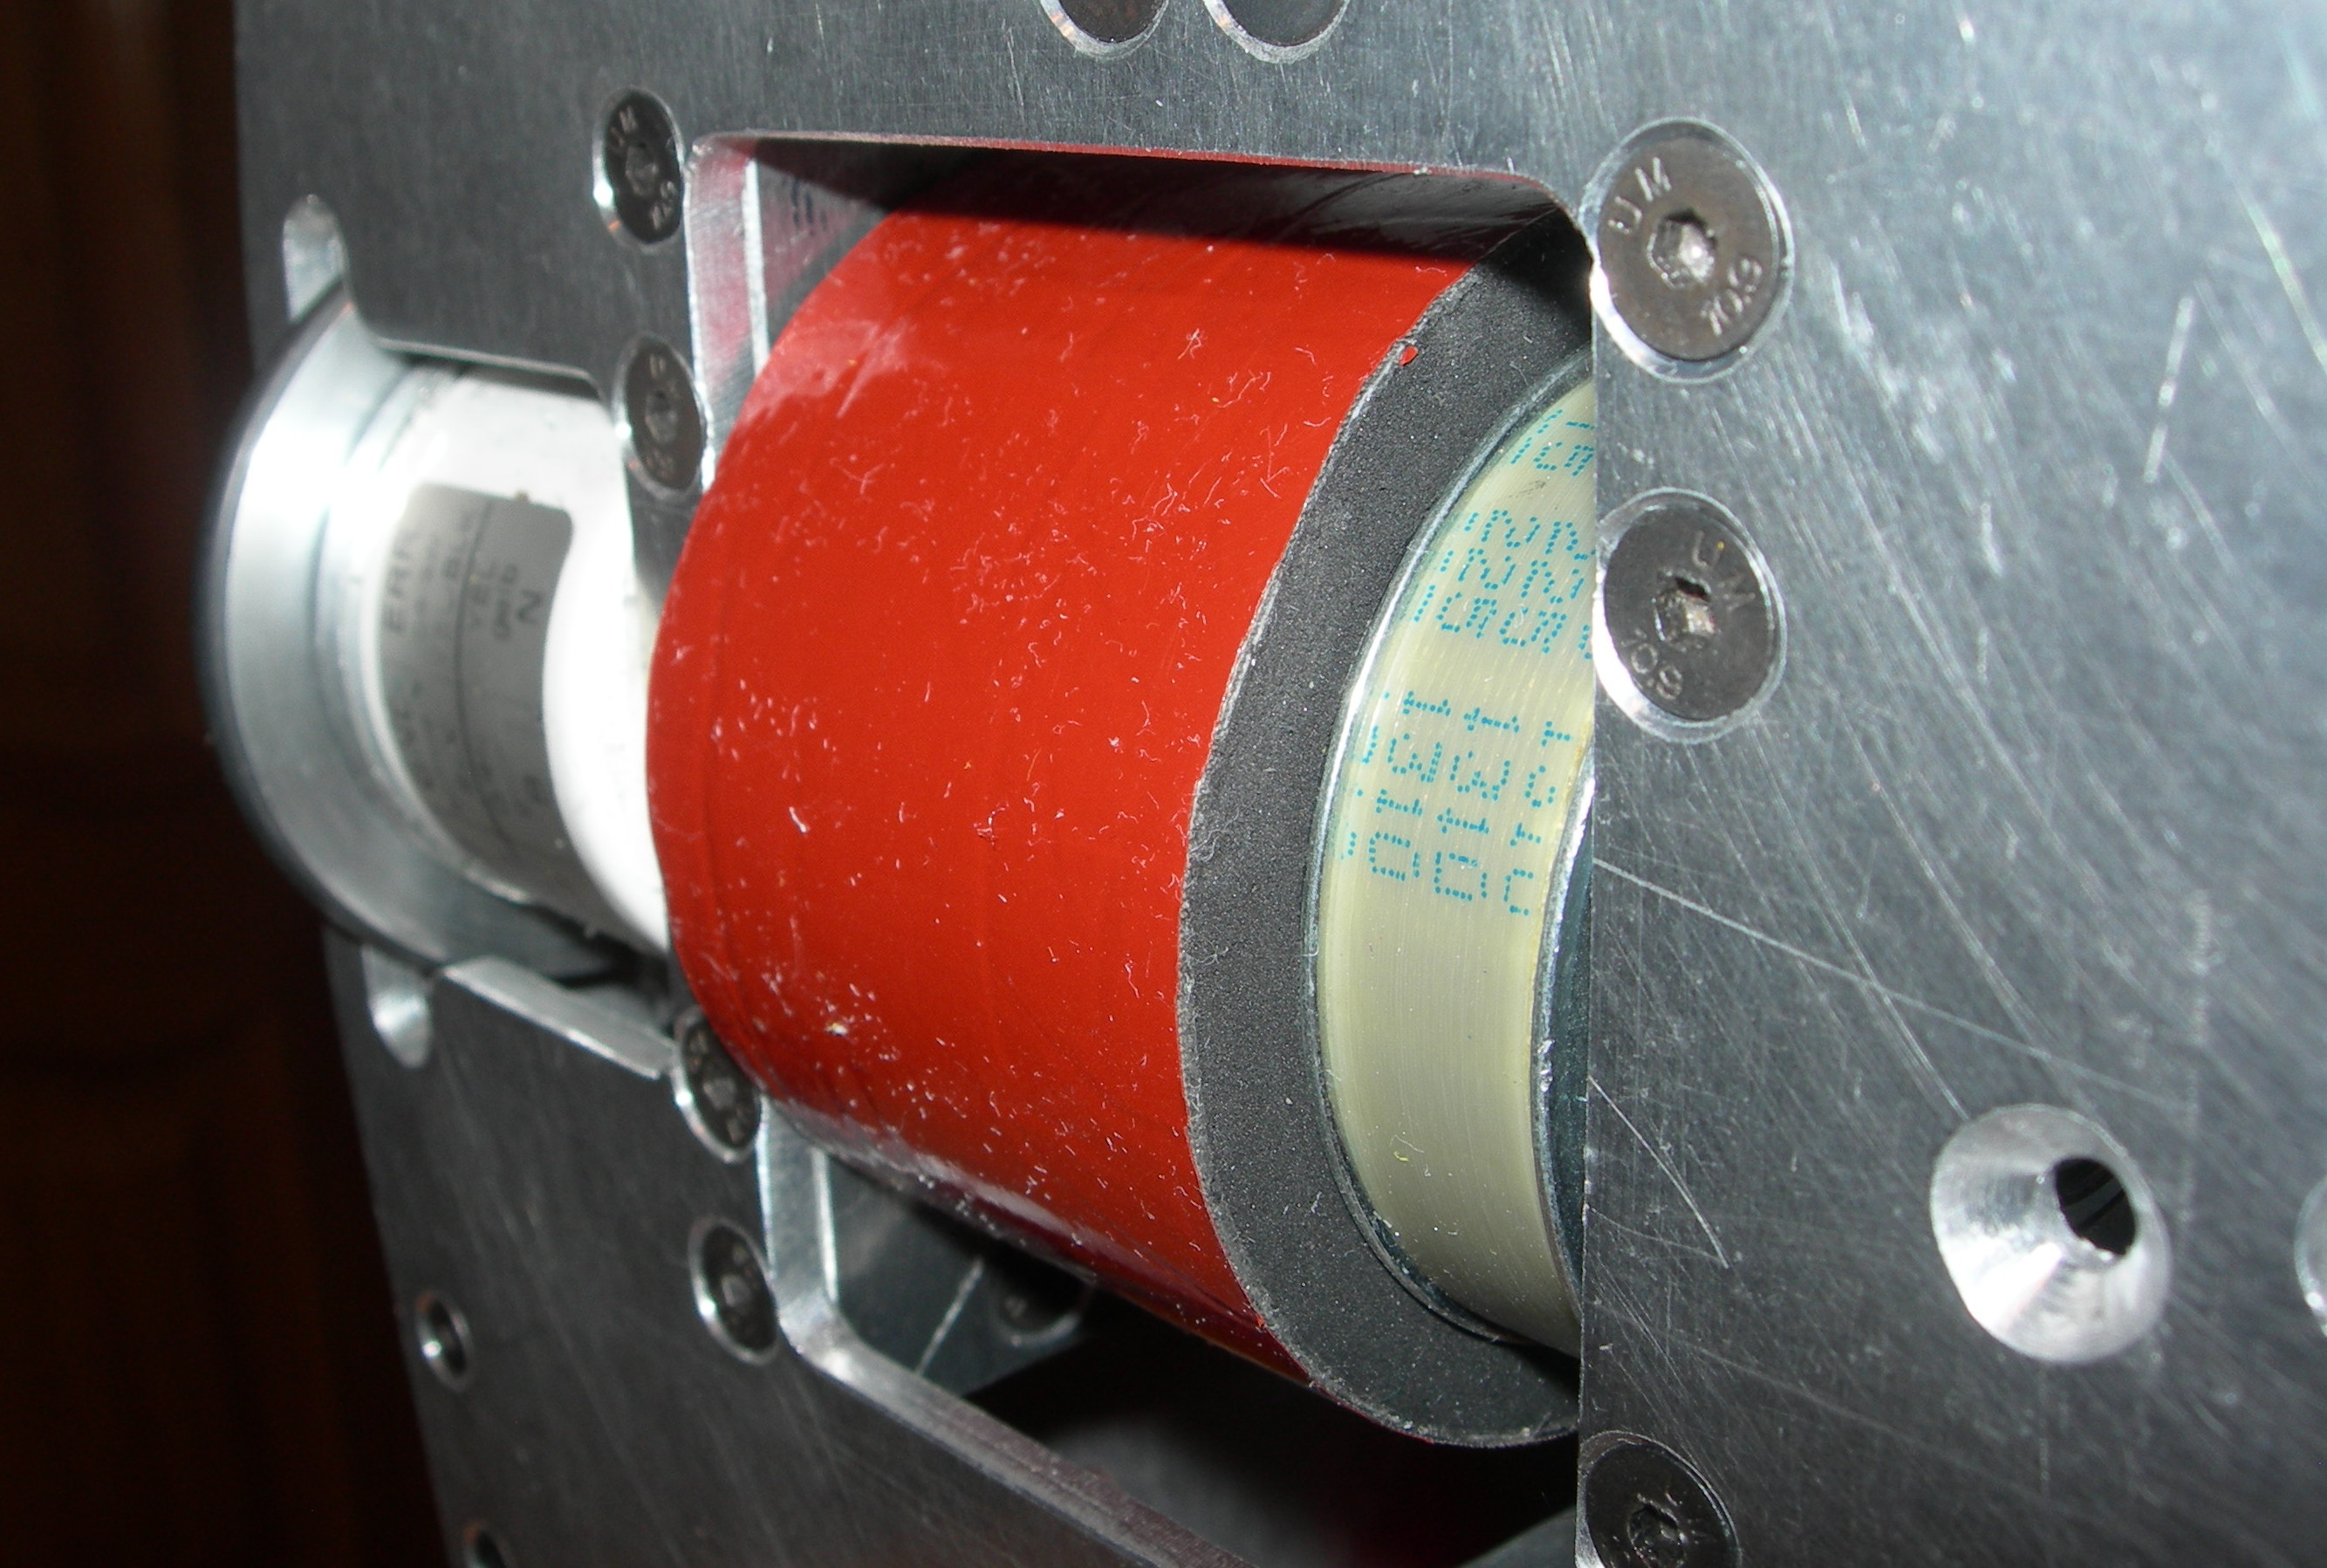
\includegraphics[height=.2\textheight]{ruedas_foam_silicona}
\caption[]{Ruedas utilizadas en los robots}
\label{fig_ruedas_foam_silicona}
\end{figure}


\subsection{Determinaci�n de la aceleraci�n m�xima en las fases de aceleraci�n y frenado}

La aceleraci�n m�xima durante las fases de aceleraci�n o frenado depende de dos condiciones. La primera es la condici�n para la cual las ruedas derrapen o deslicen. Y la segunda, en caso de robots con ruedas atr�s, es la condici�n para la cual el robot pierde contacto con el suelo en su parte delantera (como un caballo que se pone sobre sus patas trasera), pudiendo volcar hacia atr�s.

Por otro lado, el valor de la aceleraci�n m�xima para cada condici�n depende del coeficiente de adherencia de las ruedas ($K_a$) y la posici�n del centro de gravedad del robot, respecto al eje motriz y los puntos de apoyo. 

A continuaci�n describe como determinar el valor m�ximo de aceleraci�n para los siguientes tipos de robot:

\begin{enumerate}
\item Robot con ruedas atr�s
\item Robot con ruedas en el medio
\end{enumerate}

El desarrollo completo puede encontrarse en \cite{rcva_10x}. Aqu� s�lo se presentan los desarrollos que se han considerado importantes para el entendimiento la din�mica del robot y los resultados finales. Adem�s, este trabajo a�ade el resultado para el caso de un robot con ruedas en el medio asim�trico, no estudiado en \cite{rcva_10x}.

\subsubsection{Robots con ruedas atr�s}

Se parte del modelo din�mico del robot representado por la siguiente figura:

\begin{figure}[H]
\centering
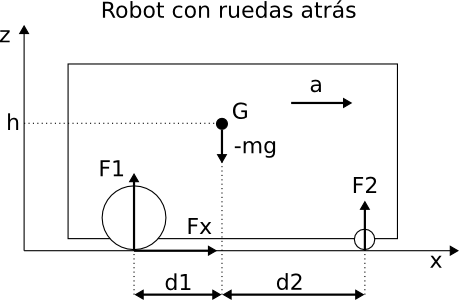
\includegraphics[width=.4\textwidth]{dinamica_a_max_ruedas_atras}
\caption[]{Modelo din�mico en fase de aceleraci�n y frenado para robots con ruedas atr�s.}
\label{fig_dinamica_a_max_ruedas_atras}
\end{figure}

Donde:
\begin{description}
\item $G$: centro de gravedad del robot.
\item $F_x$: fuerza de propulsi�n de en la rueda.
\item $F1$: fuerza normal del suelo en la rueda.
\item $F2$: fuerza normal del suelo en el punto delantero.
\item $a$: aceleraci�n del robot
\item $-mg$: fuerza de la gravedad aplicada en el centro de gravedad.
\item $d1$:  distancia entre el centro de gravedad y el eje motriz.
\item $d2$: distancia entre el centro de gravedad y el punto de apoyo delantero.
\item $d$: distancia entre el eje motriz y un punto de apoyo (d = d1 + d2).
\item $h$: altura del centro de gravedad del robot.
\end{description}

Las ecuaciones que garantiza que el sistema esta en equilibrio son las siguientes:	

\begin{description}
\item Suma de fuerzas verticales\\
\begin{equation}
\label{eq_suma_fuerzas_verticales}
2F1 + 2F2 - mg = 0
\end{equation}

\item Suma de fuerzas horizontales\\
\begin{equation}
\label{eq_suma_fuerzas_horizontales}
2F_x = ma
\end{equation}

\item Suma de torsiones aplicadas al punto G\\	
\begin{equation}
\label{eq_suma_torsiones_punto_g}
F2d2 - F1d1 + F_x \, h = 0
\end{equation}
\end{description}


A partir las ecuaciones \eqref{eq_suma_fuerzas_verticales}, \eqref{eq_suma_fuerzas_horizontales} y \eqref{eq_suma_torsiones_punto_g}	, se obtienen las ecuaciones que representan la distribuci�n de pesos en las fases de aceleraci�n y frenado:
\begin{align}
(2F1)/mg &= d2/d + (a/g)(h/d) \label{eq_distribucion_pesos_rueda}\\
(2F2)/mg &= d1/d - (a/g)(h/d) \label{eq_distribucion_pesos_apoyo}
\end{align}

Notar que el t�rmino $(2F1)/mg$ representa la distribuci�n de pesos en el eje motriz, mientras que el termino $(2F2)/mg$ representa el reparto de pesos en la parte delantera. Los t�rminos $d2/d$ y $d1/d$ representan las distribuciones de pesos en est�tico, cuando la aceleraci�n es nula ($a=0$). Y el t�rmino  $(a/g)(h/d)$ representa la transferencia de masa del robot durante la aceleraci�n o frenado.

As� pues, en fase de aceleraci�n ($a>0$) la transferencia de masa se produce hacia la parte trasera del robot por lo que el robot avanza y tiende a hacer \emph{el caballito}. Mientras que en la fase de frenado ($a<0$) la transferencia de masa se produce hacia la parte delantera de forma que las ruedas tienen a deslizar o derrapar sobre el suelo.

Se deducen algunas conclusiones al respecto:

\begin{itemize}
\item Interesa tener el m�ximo apoyo en el eje motriz aumentando el termino $(2F1)/mg$ o el termino est�tico $d2/d$, de forma que el centro de gravedad est� lo m�s cerca posible del eje motriz.

\item Cuando el t�rmino de transferencia de masa din�mica $(a/g)(h/d)$ cambia de signo debido a la aceleraci�n, se consiguen una buena fase de aceleraci�n pero una fase peor de frenado.

\item Como los robots en un partido no hacer otra cosas que acelerar y frenar, interesa reducir lo m�ximo la transferencia de masa, la cual depende �nicamente de la relaci�n $(h/d)$. Por lo tanto interesa bajar el centro de gravedad lo m�ximo posible.
\end{itemize}


Continuando con el c�lculo, la condici�n para no derrapar en la fase de aceleraci�n viene dada por la ecuaci�n \eqref{eq_fx_max_f_ka} expresada como 
\begin{equation}
\label{eq_condicion_derrape_aceleracion}
F_x < K_a \, F1
\end{equation}

y para la fase de frenado como
\begin{equation}
\label{eq_condicion_derrape_frenada}
|F_x| < K_a \, F1.
\end{equation}


Por otro lado, la condici�n para que el robot no haga \emph{el caballito} durante la fase de aceleraci�n es
\begin{equation}
\label{eq_condicion_caballito_aceleracion}
F2 > 0
\end{equation}

y para la fase de frenado es
\begin{equation}
\label{eq_condicion_caballito_frenado}
F1 > 0
\end{equation}

A partir de las ecuaciones \eqref{eq_distribucion_pesos_rueda}, \eqref{eq_distribucion_pesos_apoyo}, \eqref{eq_suma_fuerzas_horizontales} y las condiciones mencionadas anteriormente se obtienen las aceleraciones m�ximas para cada fase y condici�n.

Fase de aceleraci�n ($a>0$):
\begin{empheq}[box=\fbox]{align}
a_{max1} &= g\,\frac{K_a \, d2}{d-(K_a \, h)} \label{eq_a_max_aceleracion_derrape}\\
a_{max2} &= g\,\frac{d1}{h} \label{eq_a_max_aceleracion_caballito}
\end{empheq}


Fase de frenado ($a<0$):
\begin{empheq}[box=\fbox]{align}
a_{max1} &= g\,\frac{K_a \, d2}{d+(K_a \, h)} \label{eq_amax_frenado_derrape}\\
a_{max2} &= g\,\frac{d2}{h} \label{eq_amax_frenado_caballito}
\end{empheq}

Siendo $a_{max1}$ la aceleraci�n m�xima para no derrapar y $a_{max2}$ la aceleraci�n m�xima para no hacer \emph{el caballito}. Para cada fase, la aceleraci�n m�xima vendr� dada por el valor m�nimo de estas:
\begin{equation}
\label{eq_a_aceleracion}
a_{max} = Min\{a_{max1}, a_{max2}\}.
\end{equation}


Por ejemplo, la figura \ref{fig_ejemplo_a_max} representa el caso de dos robots iguales excepto por la altura de su centro de gravedad.	

\begin{figure}[h]
\centering
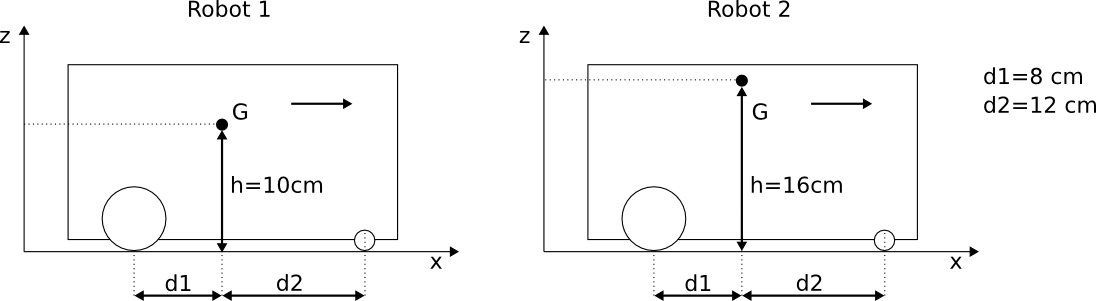
\includegraphics[width=.8\textwidth]{ejemplo_a_max}
\caption[]{Ejemplo de calculo de la aceleraci�n m�xima en las fases de aceleraci�n y frenado}
\label{fig_ejemplo_a_max}
\end{figure}

Las aceleraciones m�ximas calculadas para estos robots se muestran en la tabla \ref{tab_ejemplo_a_max}.

\begin{table}[h]
\centering
\caption{Ejemplo de aceleraciones m�ximas en funci�n del centro de gravedad}
\label{tab_ejemplo_a_max}

\begin{tabular}{ lcccc }
\hline
			& Aceleraci�n R1 & Frenado R1 & Aceleraci�n R2 & Frenado R2 \\
\hline
$a_{max1}$ 	& $1,2g$ 		& $0,4g$ 		& $3,0g$ 		& $0,3g$ 	\\
$a_{max2}$ 	& $0,8g$ 		& $1,2g$ 		& $0,5g$ 		& $0,75g$ 	\\
$a_{max}$ 	& $0,8g$ 		& $0,4g$ 		& $0,5g$ 		& $0,3g$ 	\\
			& ($8\,m/s$) 		& ($4\,m/s$) 		& ($5\,m/s$) 		& ($3\,m/s$)  \\
\hline
\end{tabular}

\end{table}

Observar que estos c�lculos s�lo se refieren a desplazamientos de translaci�n y no a giros, permitiendo maximizar la aceleraci�n. Que el robot sea capaz de alcanzar dicha aceleraci�n va a depender de la elecci�n de los motores y su reductora.

Por otro lado, hay que tener en cuenta que estos c�lculos dependen �nicamente del centro de gravedad del robot y del coeficiente de adherencia de las ruedas. El peso del robot no interviene.


\subsubsection{Robots con ruedas en el medio}

Un robot que tiene las ruedas en el medio puede ser que tenga su centro de gravedad exactamente sobre el eje motriz, de forma que el robot es sim�trico. Si el centro de gravedad esta desplazado se habla de un robot asim�trico.

Los modelos din�micos para estos casos se corresponden con la siguiente figura:

\begin{figure}[H]
\centering
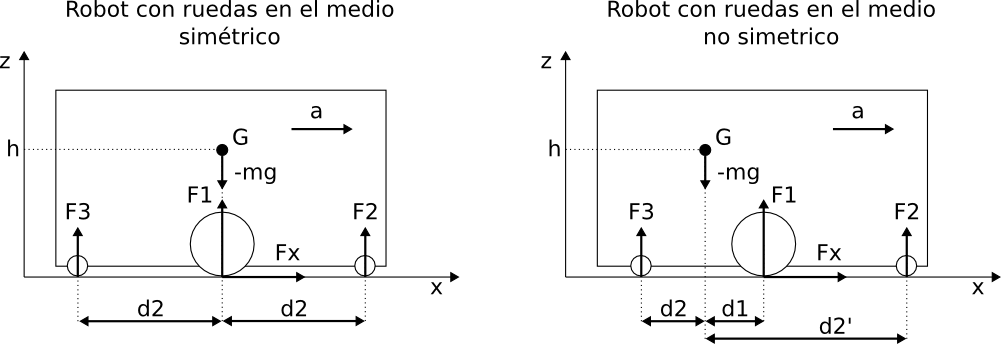
\includegraphics[width=.8\textwidth]{dinamica_a_max_ruedas_medio}
\caption[]{Modelo din�mico fase de aceleraci�n y frenado para robots con ruedas en el medio.}
\label{fig_dinamica_a_max_ruedas_medio}
\end{figure}

Donde:
\begin{description}
\item $G$: centro de gravedad del robot.
\item $F_x$: fuerza de propulsi�n de en la rueda.
\item $F1$: fuerza normal del suelo en la rueda.
\item $F2$: fuerza normal del suelo en el punto delantero.
\item $F3$: fuerza normal del suelo en el punto de apoyo trasero.
\item $a$: aceleraci�n del robot
\item $-mg$: fuerza de la gravedad aplicada en el centro de gravedad.
\item $d1$: distancia entre el centro de gravedad y el eje motriz.
\item $d2$: distancia entre el centro de gravedad y el punto de apoyo trasero.
\item $d2'$: distancia entre el centro de gravedad y el punto de apoyo delantero.
\item $h$: altura del centro de gravedad del robot.
\end{description}

Para el caso del robot sim�trico de la figura \ref{fig_dinamica_a_max_ruedas_atras} y siguiendo un an�lisis igual al realizado para robots con ruedas atr�s, se obtienen las ecuaciones que definen las aceleraciones m�ximas. Debido a que el robot tiene 4 puntos de apoyo no es posible que �ste haga \emph{el caballito}, por lo que la aceleraci�n m�xima vendr� dada �nicamente para la condici�n de derrape de las ruedas y es la misma para las fases de aceleraci�n y frenado dada la simetr�a del robot:
\begin{equation}
\label{eq_a_max_simetrico}
\boxed{a_{max} = g\,\frac{K_a}{1 + K_a\,(h/d2)}}
\end{equation}


Por otro lado, en el caso del robot asim�trico, el centro de gravedad cae entre el eje motriz y los puntos de apoyo de uno de los extremos del robot. Al igual que en el caso anterior la condici�n de hacer \emph{el caballito} no existe al tener el robot 4 puntos de apoyo. Sin embargo, la aceleraci�n m�xima es distinta para la fase de aceleraci�n y la de frenado debido a la asimetr�a del robot.

Fase de aceleraci�n ($a>0$):
\begin{equation}
\label{eq_a_max_pos_no_simetrico}
\boxed{a_{max} = g\,\frac{K_a}{(d1+d2)/d2 + K_a\,(h/d2)}}
\end{equation}


Fase de frenado ($a<0$):
\begin{equation}
\label{eq_a_max_neg_no_simetrico}
\boxed{a_{max} = g\,\frac{K_a}{(d2'-d1)/d2' + K_a\,(h/d2')}}
\end{equation}

Se comprueba que si $d1=0$, el modelo se corresponde con el de un robot sim�trico y las ecuaciones \eqref{eq_a_max_pos_no_simetrico} y \eqref{eq_a_max_neg_no_simetrico} coinciden con la ecuaci�n \eqref{eq_a_max_simetrico}.

\subsubsection{Medida del centro de gravedad del robot}

Se ha visto que para los c�lculos de la aceleraci�n m�xima del robot es necesario conocer la posici�n del centro de gravedad del mismo. Su valor puede ser medido f�cilmente utilizando una regla y una barra lo suficientemente larga. Por ejemplo para medir la altura del centro de gravedad se proceder�a a apoyar el robot sobre la barra por una de sus caras como muestra la figura \ref{fig_medida_centro_gravedad} hasta dar con una posici�n en la que el robot se encuentre en equilibrio. Una vez obtenida la posici�n de equilibrio se mide la distancia que hay de la base del robot al centro de la barra, la cual se corresponde con la altura del centro de gravedad. 

\begin{figure}[h]
\centering
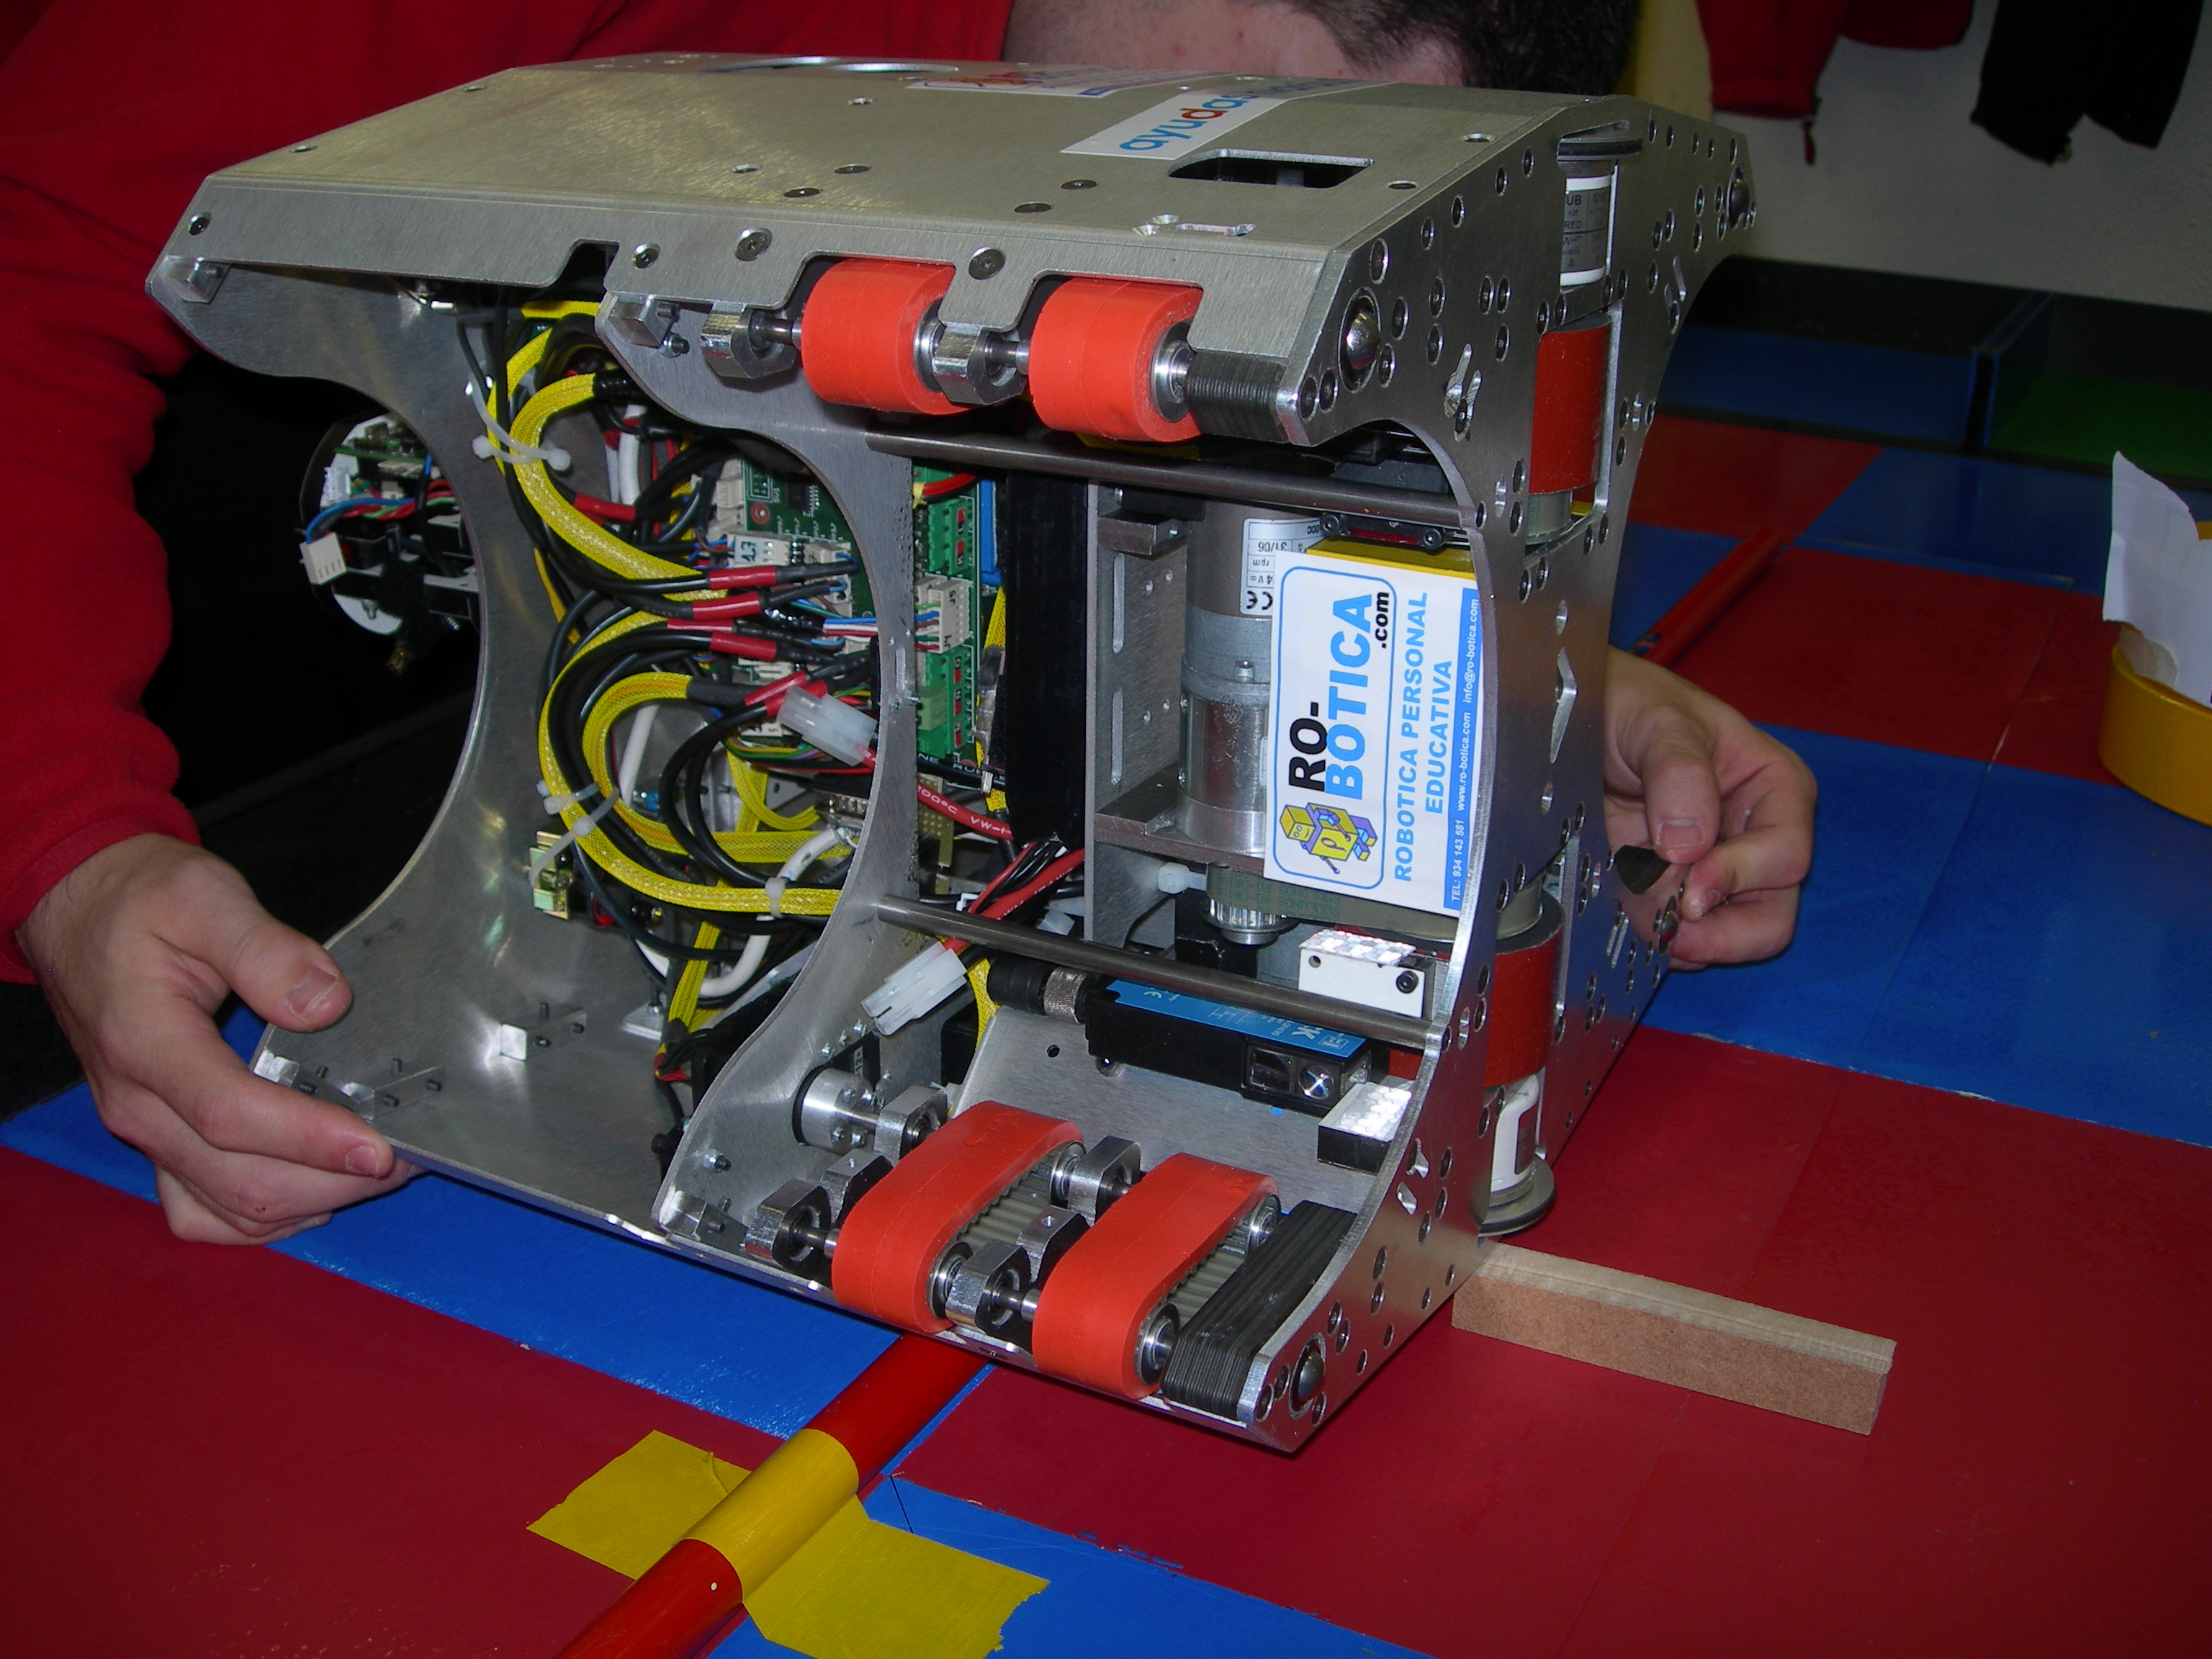
\includegraphics[width=.4\textwidth]{medida_centro_gravedad}
\caption[]{Ejemplo de medida de la altura del centro de gravedad del robot}
\label{fig_medida_centro_gravedad}
\end{figure}

La operaci�n se repite sobre la base del robot situando la barra paralela al eje motriz, de forma que se determina la distancia del centro de gravedad a dicho eje. Y por �ltimo, se puede realizar la medida con la barra situada perpendicularmente al eje motriz con el fin de comprobar que el robot es sim�trico en dicho eje y que el peso soportado por cada rueda es el mismo.

\subsection{Perfil de velocidad trapezoidal}

Como ya se ha visto, el desplazamiento de un robot sobre un plano horizontal se divide en una fase de aceleraci�n, otra de frenado y una fase intermedia de velocidad constante. Dichas fases se suelen implementar mediante un perfil trapezoidal de velocidad como el representado en la figura \ref{fig_perfil_trapezoidal}. 

\begin{figure}[h]
\centering
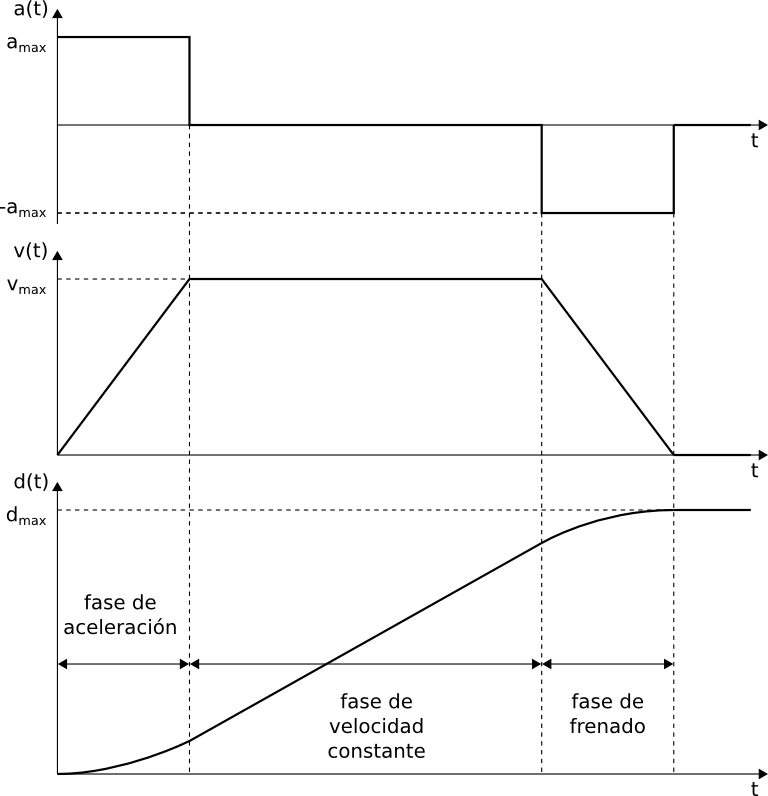
\includegraphics[width=.8\textwidth]{perfil_trapezoidal}
\caption[]{Fases de un perfil trapezoidal de velocidad: aceleraci�n, velocidad y distancia recorrida}
\label{fig_perfil_trapezoidal}
\end{figure}

%En dicho perfil se pueden identificar las fases de aceleraci�n, velocidad constante y frenado. A cada una de estas fases le corresponde una distancia recorrida ($d1,d2,d3$) y un tiempo ($t1,t2,t3$).

Como se sabe, la optimizaci�n de dicho perfil pasa por la determinaci�n de las aceleraciones y velocidad m�ximas. La aceleraci�n m�xima se corresponde con aquella para la que el robot se encuentre al limite del deslizamiento o de hacer \emph{el caballito} y se calcula de la forma que se ha descrito en la secci�n anterior. En la pr�ctica, nunca se trabaja con la aceleraci�n m�xima te�rica y si no que se utiliza una aceleraci�n de seguridad que suele se el 80\% de la te�rica:
\begin{equation}
\label{eq_a_seguridad}
a = 0.8\,a_{max}
\end{equation}

Respecto a la velocidad m�xima, depender� en �ltima medida del motor y la reductora utilizada. No obstante, dadas las dimensiones del campo y que los robots han de ser capaces de evitar colisiones entre ellos, una velocidad de $1m/s$ suele ser un buen valor de compromiso.

Resulta interesante el an�lisis que hacen en \cite{rcva_10x} sobre el valor de la velocidad m�xima. En este an�lisis se comparan dos perfiles trapezoidales de distinta velocidad ($1m/s$ y $1,4m/s$), de igual aceleraci�n ($a=2\,m/s$) y para una misma distancia recorrida ($1m/s$). El resultado es que el perfil con velocidad de $1,4m/s$ tarda s�lo $0,1s$ menos en recorrer la distancia de $1m$. Un tiempo que es despreciable. Esto es debido a que el tiempo de la fase de velocidad constante del perfil de $1.4m/s$ es muy peque�o respecto al tiempo que se invierte en acelerar y frenar. De esto se deduce que para distancias cortas no es tan importante la velocidad como la aceleraci�n del robot.

Por �ltimo,respecto a la gr�fica de distancia del perfil trapezoidal, se observa una evoluci�n parab�lica durante las fases de aceleraci�n y frenado que permite un movimiento suave del robot. Como se ver� en la secci�n \ref{sec_control_posicion}, esta curva representa una consigna de distancia para el sistema de control de posici�n.

\subsection{Dimensionamiento de la reductora}

Como se sabe, las ruedas del eje motriz se encuentran conectadas al motor por medio de una reductora. El modelo mec�nico de dicho sistema se muestra en la figura \ref{fig_modelo_reductora_motor}. 

\begin{figure}[H]
\centering
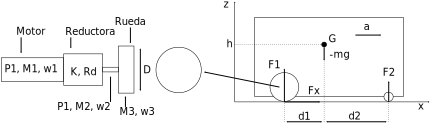
\includegraphics[width=.8\textwidth]{modelo_reductora_motor}
\caption[]{Modelo mec�nico de uno de los motores del sistema de tracci�n diferencial.}
\label{fig_modelo_reductora_motor}
\end{figure}

Donde:
\begin{description}
\item $\omega_i$: velocidades angulares ($rad/s$)
\item $M_i$: par o momentos de fuerza ($N\,m$)
\item $P_i$: potencias mec�nicas ($Nm/(rad/s)$)
\item $K$: relaci�n de reducci�n de la reductora
\item $Rd$: rendimiento de la reductora
\item $D$: di�metro de la rueda
\end{description}

La potencia mec�nica en el motor $P1$ y en el eje de salida de la reductora $P2$ viene dada como:
\begin{align}
P1 &= M1\,\omega1 \label{eq_potencia_mecanica_motor} \\
P2 &= M2\,\omega2 \label{eq_potencia_mecanica_reductora}
\end{align}

Dichas potencias se relacionan mediante la reductora de la siguiente manera:
\begin{align}
\omega2 &= \frac{\omega1}{K} \label{eq_relacion_w1_w1} \\
M2 &= M1\,Rd\,K \label{eq_relacion_M2_M1} \\
P2 &= P1\,Rd \label{eq_relacion_P2_P1} 
\end{align}

Observar que la relaci�n entre potencias en \eqref{eq_relacion_P2_P1} no depende de $K$. Si $K$ aumenta el par de la reductora $M2$ aumenta pero la velocidad $w2$ disminuye.	

Por otro lado, del modelo del motor de corriente continua se sabe que la tensi�n de armadura del motor $U$ y el par motor $M$ vienen dados por las expresiones:
\begin{align}
U &= r\,i + K_v\,\omega \label{eq_tension_armadura} \\
M &= K_m\,i \label{eq_par_motor}
\end{align}

Siendo:
\begin{description}
\item $r$: resistencia de la armadura ($\Omega$)
\item $i$: corriente de la armadura (A)
\item $K_v:$ constante de fuerza electromec�nica (V/(rad/s))
\item $K_m$: constante de par motor (Nm/A)
\end{description}

A la hora de dimensionar la reductora se busca determinar el valor de reducci�n ($K$) que genere un par suficiente en la rueda para vencer las fuerzas aplicadas en la misma que se oponen al movimiento.

No obstante existe una condici�n m�s restrictiva a la hora de dimensionar la reductora. Es el caso en el que las ruedas queden bloqueadas debido a que el robot se encuentra con un obst�culo imprevisto. Por ejemplo una pared debido a un error de posicionamiento, o que haya un objeto inesperado entre el robot y la pared. En ese caso el controlador de posici�n reaccionar� aumentando la tensi�n del motor hasta su valor m�ximo $U_{max}$ (tensi�n de saturaci�n $v_{sat}$) y se corre el riesgo de que el motor se queme. Este caso es analizado en \cite{rcva_10x} a partir de modelo t�rmico del motor. El an�lisis determina que en caso de bloqueo de una rueda la vida �til del motor es de 2,3s, a menos que el driver del motor sirva de fusible y se rompa antes o que exista un mecanismo de protecci�n.

Teniendo en cuenta este caso, un dimensionamiento m�s correcto de la reductora es aquel que permita que las ruedas derrapen antes de que la tensi�n del motor alcance su valor m�ximo.

Por un lado se calcula el par en el motor $M1$ necesario para producir deslizamiento a partir del par en la rueda $M3$, el cual depende de a su vez la fuerza de propulsi�n m�xima de las ruedas $F_{x\,max}$.
\begin{align}
M1 &= \frac{M3}{K\,Rd} \label{eq_M1} \\
M3 &= F_{x\,max}\,\frac{D}{2} \label{eq_M3} \\
F_{x\,max} &= \frac{K_a\,F1}{2} \label{eq_fx_max}
\end{align}

La fuerza aplicada sobre las ruedas $F1$ depende de la distribuci�n de pesos sobre el eje motriz y se corresponde con el peso $P1$ medido durante el la medida experimental del coeficiente de adherencia $K_a$. De forma general $F1$ se calcula como:
\begin{equation}
F1 = mg\,\frac{d2}{d} \label{eq_F1}
\end{equation}

El par en el motor $M1$ resulta:
\begin{equation}
M1 = \frac{K_a\,mg\,(d2/d)}{K\,Rd\,D}
\end{equation}


Por otro lado, a partir de las ecuaciones del modelo del motor \eqref{eq_tension_armadura} y \eqref{eq_par_motor}, se obtiene el par m�ximo que puede dar el motor a la salida de la reductora $M2$ para la situaci�n de bloqueo ($\omega = 0$):
\begin{align}
U &= U_{max} = v_{sat} \label{eq_v_{sat}} \\
i|_{\omega = 0} &= \frac{v_{sat}}{r} \label{eq_i_w_zero} \\
M2 &= K_m\,i = K_m\,\frac{v_{sat}}{r} \label{eq_M2}
\end{align}


La condici�n que garantiza el deslizamiento de las ruedas en una situaci�n de bloqueo es que el par m�ximo del motor sea mayor que el par en el l�mite de deslizamiento de la rueda. Para asegurar dicha condici�n se a�ade un margen de un 20\% de forma que el deslizamiento sea apreciable:
\begin{equation}
M2 >= 1,2\,M1 \label{eq_condicion_kmin}
\end{equation}

El valor m�nimo de la reductora $K_{min}$ se obtiene al sustituir \eqref{eq_M1} y \eqref{eq_M2} en \eqref{eq_condicion_kmin} y despejar $K$:
\begin{equation}
\boxed{K_{min} = 1,2\,\frac{K_a\,mg\,(d2/d)\,D\,r}{4\,K_m\,Rd\,v_{sat}}} \label{eq_kmin}
\end{equation}

Notar que $K_{min}$ aumenta si los t�rminos $K_a\,F1$, $D$ o $r$ aumentan, o $K_m$, $U_{max}$ disminuye.

Por ejemplo, el sistema de tracci�n diferencial de la plataforma desatollada utiliza unos motores \emph{brushless} Dunkermotoren BG40x50 alimentados a 24V de 30W. Aunque no se trata de un motor de corriente continua se sabe por \cite{bercerra14} que se puede modelizar como tal y que su funcionamiento queda representado por las mismas curvas del motor de continua como muestra la figura \ref{fig_motor_bg40x50_curvas}

\begin{figure}[h]
\centering
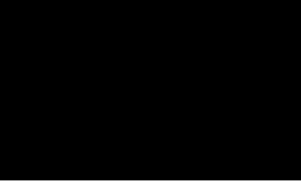
\includegraphics[width=.8\textwidth]{motor_bg40x50_curvas}
\caption[]{Curvas del motor Dunkermotoren BG40x50 24V dada por el fabricante.}
\label{fig_motor_bg40x50_curvas}
\end{figure}

\begin{figure}[h]
\centering
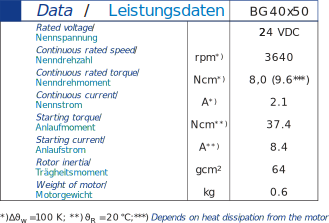
\includegraphics[width=.6\textwidth]{motor_bg40x50_tabla}
\caption[]{Par�metros del motor Dunkermotoren BG40x50 24V dadas por el fabricante.}
\label{fig_motor_bg40x50_tabla}
\end{figure}

A partir de los par�metros y curvas dadas por el fabricante (ver figura \ref{fig_motor_bg40x50_tabla} y \ref{fig_motor_bg40x50_curvas}) se deducen las variables necesarias para el c�lculo de la reductora. La resistencia equivalente se obtiene de \eqref{eq_tension_armadura} a partir del la tensi�n nominal $U_n$ y la corriente de arranque $i_o$ como

$$r = \frac{U_n}{i_o} = \frac{24V}{8,4A} = 2,86\Omega$$

Por otro lado la constante mec�nica $K_m$ se obtiene a partir de la pendiente de la recta $i=f(M)$ de la figura \ref{fig_motor_bg40x50_curvas} los puntos $(M_n, i_n)$ y $(M_o, i_o)$ como:

$$ K_m = \frac{M_o - M_n}{i_o - i_n} =  \frac{(37,4-8)[Ncm]}{(8,4-2,1)[A]} \times \frac{1[m]}{100[cm]} = 46,7 mN\,m/A $$

Adem�s seg�n el fabricante las reductoras compatibles para esta motor tienen un rendimiento $Rd$ de un 90\% hasta valores de $K=8$


Para el caso del robot P.Tinto (Eurobot 2015) sus datos son:
\begin{align*}
m &= 15 Kg\\
D &= 0,6 m\\
d &= 0,131 m\\
d2 &= 0,112 m\\
K_a &= 1\\
V_{bat}&= 24V
\end{align*}

Por �ltimo, sustituyendo en \eqref{eq_kmin} se obtiene un valor de 
$$K_{min} = 6,37.$$ 
Puesto que es menor que 8 el rendimiento utilizado de la reductora es v�lido. La reductora del fabricante de valor cercano por exceso es la reductora PLG42S 8:1. 

En el caso real, ya se dispon�an de estos motores y adem�s ya ven�an con una reductora PLG42S de factor de reducci�n 4:1\footnote{Estos motores se compraron en el a�o 2010 a un vendedor de eBay. Los motores nuevos son caros y por que entonces no hab�a presupuesto suficiente para comprar unos nuevos a demanda de los requisitos del robot.}. Se opt� por a�adir una segunda etapa de reducci�n. Esta segunda etapa se implemento mediante una reducci�n por correa dentada, cuyo rendimiento es del 90\%. Recalculando $K_{min}$ para un rendimiento de $0,9�$ se obtiene una 
$$K_{min} = 7.$$	

A partir de este valor, se escogi� un factor de reducci�n 2:1 para la segunda etapa obteniendo un factor de reducci�n total de 8:1.

\subsection{Calculo de la velocidad m�xima}

Asumiendo que los motores del robot tienen asociado un controlador de posici�n o velocidad, el dimensionamiento de estos se realiza de forma que el controlador no llegue nunca a la tensi�n de saturaci�n. Esto es, la tensi�n $U$ de los motores ha de estar por debajo de la tensi�n de saturaci�n $v_{sat}$. Interesa conocer cual es el margen entre estas dos tensiones necesario para realizar un control sobre los motores sin bloqueos.

El an�lisis a realizar parte de la premisa de utilizar un perfil de velocidad trapezoidal. Para ello se considera que el perfil de velocidad constituye una consigna de velocidad para el controlador \cite{rcva_10x}.

El an�lisis parte del perfil perfil de velocidad representado en la figura \ref{fig_dimensionamiento_motores} y de las ecuaciones que describen el modelo del motor de continua
\begin{align}
U &= r\,i + K_v\,\omega,\label{eq_tension_armadura2} \\
M &= K_m\,i \label{eq_par_motor2}
\end{align}


\begin{figure}[h]
\centering
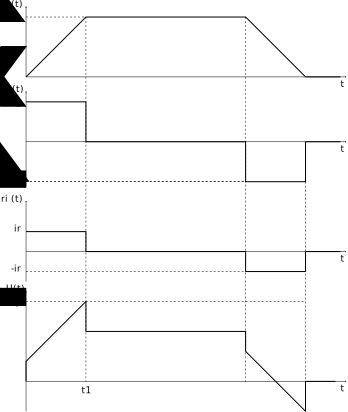
\includegraphics[width=.7\textwidth]{dimensionamiento_motores}
\caption[]{Tensi�n de armadura del motor en el l�mite de saturaci�n para un perfil de velocidad trapezoidal.}
\label{fig_dimensionamiento_motores}
\end{figure}

Se observa que durante las fases de aceleraci�n y frenado la aceleraci�n del robot es constante, por lo que el par motor\footnote{$M=F\times\,d = m\,a\times\,d$. Si $a=\text{cte}$, $M=\text{cte}$} y la corriente son constantes\footnote{$M=K_m\,i$. Si $M=\text{cte}$, $i=\text{cte}$}. La tensi�n de armadura $U$ del motor es la suma del termino �hmico $r\,i$ y del termino de velocidad angular $K_v\,\omega$. Por lo tanto durante las fases de aceleraci�n y frenado, el t�rmino �hmico ser� constante y el t�rmino de velocidad proporcional a esta. De esta forma el valor m�ximo de la tensi�n de armadura del motor $U$ se alcanza, al final de la fase de aceleraci�n, en el instante $t1$.

Por otro lado, hay que recordar que el calculo de la reductora tambi�n se realiza en base a la tensi�n de saturaci�n $V_{sat}$, para la cual las ruedas comenzar�an a deslizar para evitar el bloqueo del motor. Es por ello que el instante $t1$ constituye el punto m�s cr�tico de las fases del perfil trapezoidal.

El l�mite de funcionamiento sin saturaci�n es dado por la ecuaci�n \eqref{eq_tension_armadura2}, valida en el instante $t1$. Por un lado, la corriente de armadura $i$ se puede expresar en funci�n de la aceleraci�n $a$ del robot del siguiente modo:
\begin{equation}
\begin{split}
i &= \frac{M1}{K_m}\\
M1 &= \frac{M3}{K\,Rd}\\
M3 &= Fx\,\frac{D}{2}\\
2Fx &= m\,a \label{eq_desarrollo_i_func_a}
\end{split}
\end{equation}

Por otro lado, la velocidad angular $\omega$ se puede expresar en funci�n de la velocidad $v$ del robot como:
\begin{equation}
\begin{split}
\omega1 &= K\,\omega3\\
v &= \frac{2\omega3}{D} \label{eq_w_func_v}
\end{split}
\end{equation}

Sustituyendo los desarrollos \eqref{eq_desarrollo_i_func_a} y \eqref{eq_w_func_v} en \eqref{eq_tension_armadura2} se obtiene\footnote{$K_v$ ha sido sustituido por $K_m$ ya que coinciden si ambas constantes se expresan en $[V/(rad/s)]$ y $Nm/A$, respectivamente}:
\begin{equation}
U = \Big(\frac{r\,m\,D}{4K\,Rd\,K_m}\Big)\,a + \Big(\frac{2K_m\,K}{D}\Big)\,v \label{u_func_a_v}
\end{equation}

Representando la velocidad $v$ en funci�n de la aceleraci�n $a$ se obtiene la ecuaci�n de la recta 
\begin{equation}
v = v_o - \frac{v_o}{a_o}\,a \label{v_func_a}
\end{equation}

Donde
\begin{align}
v_o &= \frac{\,U\,D}{2K\,K_m} \label{v_o} \\ 
a_o &= \frac{4K\,U\,Rd\,K_m}{r\,D\,m} \label{a_o}
\end{align}

Dicha recta se representa en la figura \ref{fig_recta_velocidad_maxima}, donde se puede observar que la aceleraci�n m�xima $a_{max}$ define la zona �til de funcionamiento sin saturaci�n y deslizamiento. 

\begin{figure}[p]
\centering
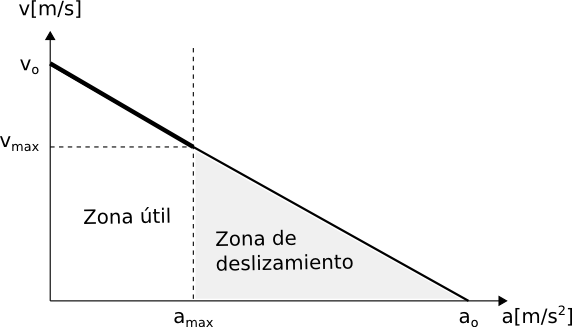
\includegraphics[width=.65\textwidth]{recta_velocidad_maxima}
\caption[]{Recta de velocidad m�xima para una aceleraci�n dada y zona �til de funcionamiento sin saturaci�n y deslizamiento.}
\label{fig_recta_velocidad_maxima}
\end{figure}

\begin{figure}[p]
\centering
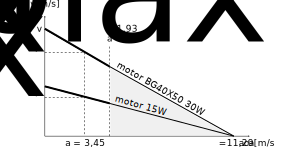
\includegraphics[width=.7\textwidth]{recta_velocidad_maxima_ptinto}
\caption[]{Velocidad y aceleraci�n del robot P.Tinto para un funcionamiento sin saturaci�n y deslizamiento.}
\label{fig_recta_velocidad_maxima_ptinto}
\end{figure}

Recapitulando y simplificando \eqref{v_func_a}, la velocidad m�xima del robot $v_{max}$ al l�mite de saturaci�n y deslizamiento para una aceleraci�n dada se obtiene a partir de la expresi�n
\begin{empheq}[box=\fbox]{align}
v_{max} &= v_o\, (1-\frac{a_{max}}{a_o}) \label{v_max_func_a_max}\\
v_o &= \frac{\,U\,D}{2K\,K_m} \label{v_o} \\ 
a_o &= \frac{4K\,U\,Rd\,K_m}{r\,D\,m} \label{a_o}
\end{empheq}

Siguiendo con el ejemplo del dimensionamiento de la reductora del robot P.Tinto, a partir de los datos ya conocidos del motor Dunkermotoren BG40x50 y de las expresiones \eqref{v_o} y \eqref{a_o}, se obtiene la recta velocidad-aceleraci�n representada en la figura \ref{fig_recta_velocidad_maxima_ptinto} donde 
\begin{align}
v_o &=  1,93 m/s \label{v_o_ptinto} \\ 
a_o &=  11,29 m/s^2\,\,(1,15g)\label{a_o_ptinto}
\end{align}

P.Tinto es un robot tipo con ruedas en el medio no sim�trico como el de la figura \ref{fig_dinamica_a_max_ruedas_medio}. A partir del coeficiente de adherencia de las ruedas $K_a = 1$ y las medidas del centro de gravedad respecto al eje motriz:
\begin{equation}
\begin{split}
d1 &= 19,18 mm\\
d2 &= 111,8 mm\\
d2' &= 139,68 mm\\
h &= 122,9 mm
\end{split}
\end{equation}

Mediante las ecuaci�nes \eqref{eq_a_max_neg_no_simetrico} y \eqref{eq_a_max_pos_no_simetrico} se determina una aceleraci�n m�xima 
\begin{equation}
a_{max} = 0,44g\,\,(4,32m/s�)
\end{equation}

Teniendo en cuenta un margen de seguridad del 20\% se fija la aceleraci�n del robot a un valor de $0,35g$ ($3,45 m/s^2$). A partir de la ecuaci�n \eqref{v_max_func_a_max} se obtiene la velocidad correspondiente para un funcionamiento sin saturaci�n y deslizamiento:
\begin{equation}
v_{max} = 1,2 m/s
\end{equation}


Se ha representado una segunda recta en la figura \ref{fig_recta_velocidad_maxima_ptinto} correspondiente a un motor de la mitad de potencia. Observar que para una misma aceleraci�n la velocidad es menor. En el primer caso la velocidad es superior a la velocidad deseada ($1 m/s$) y el motor BG40x50 es v�lido, mientras que en el segundo caso el motor no ser�a valido.

La gr�fica de la figura \ref{fig_perfil_vmax_amax} muestra el resultado de aplicar un perfil trapezoidal cuya velocidad es la m�xima calculada. Observar que al final de la fase de aceleraci�n la tensi�n de control de los motores se encuentra muy cerca de su valor de saturaci�n (63500). Si se disminuye la velocidad hasta $0,8m/s$, el valor de la tensi�n baja hasta el $80\%$ de su m�ximo, como muestra la figura \ref{fig_perfil_v08_amax}.

\begin{figure}[p]
\centering
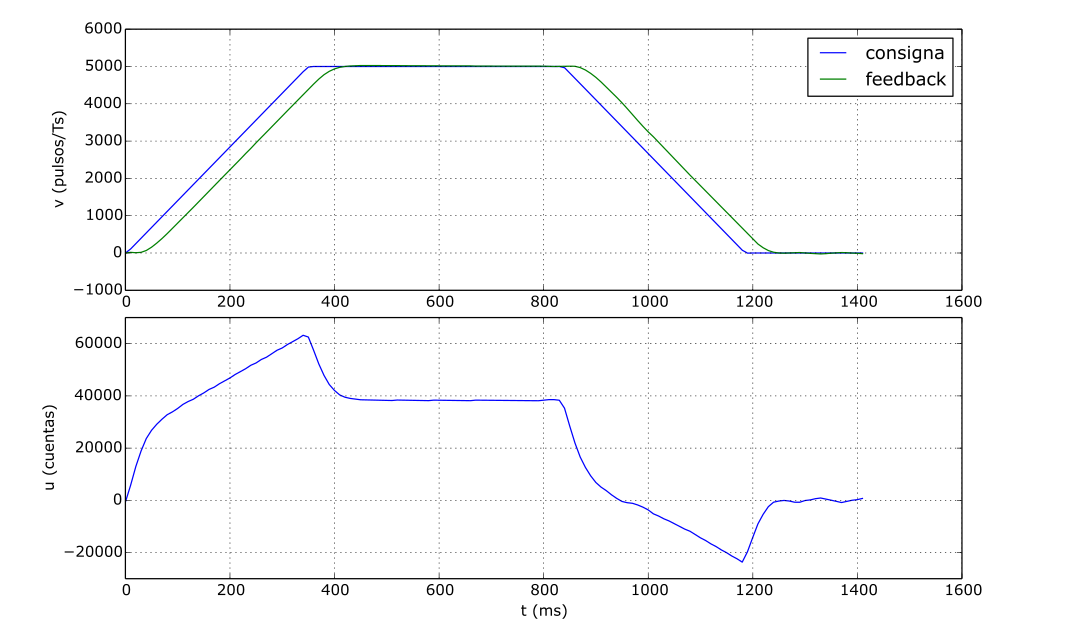
\includegraphics[width=\textwidth]{perfil_vmax_amax}
\caption[]{Se�al de control de los motores para un perfil de velocidad trapezoidal de $0,8m/s$ y una aceleraci�n de $3,45m/s$}
\label{fig_perfil_vmax_amax}
\end{figure}

\begin{figure}[p]
\centering
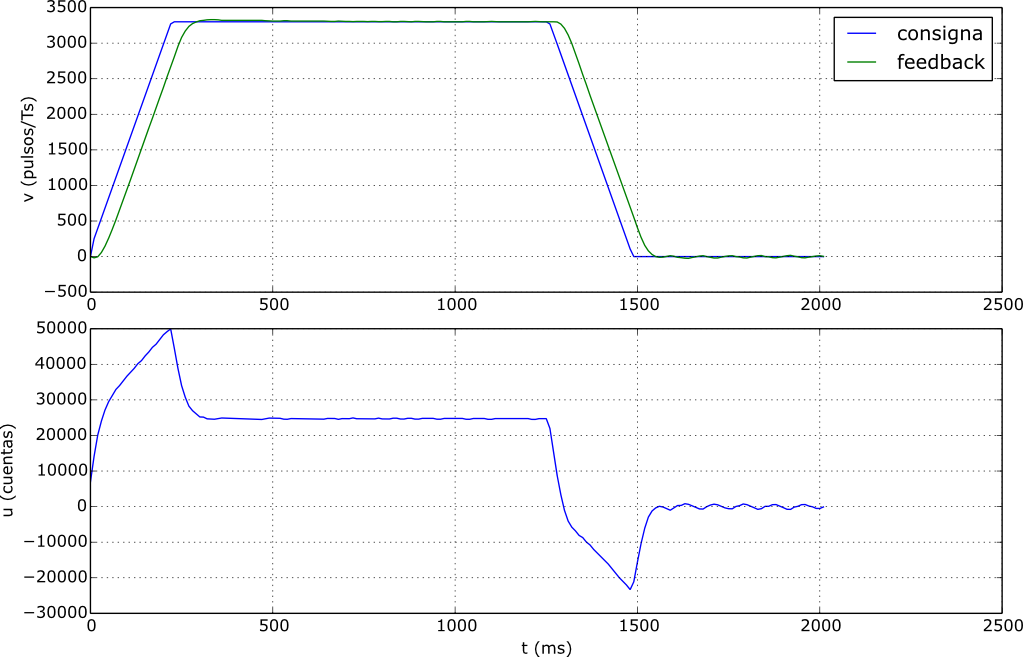
\includegraphics[width=\textwidth]{perfil_v08_amax}
\caption[]{Se�al de control de los motores para un perfil de velocidad trapezoidal de $0,8m/s$ y una aceleraci�n de $3,45m/s$}
\label{fig_perfil_v08_amax}
\end{figure}



%\subsection{Resultados experimentales}
%\vfill
%\newpage

\section{Control en posici�n de tipo polar}
\label{sec_control_posicion}

La plataforma rob�tica base implementa un control de posici�n de tipo polar. Este tipo de control es muy  utilizado por los robots de Eurobot y es el que mejor se adapta a este tipo de aplicaci�n, ya que, en ultima medida el robot ha de ser capaz de llegar a posiciones espec�ficas del campo donde manipular elementos de juego. As� mismo, este tipo de control de posici�n ha sido muy comentado en los foros de Eurobot \cite{foros_eurobot}, documentado \cite{rcva_10x} \cite{rcva_asserv} e implementado por muchos equipos \cite{microb}.

La posici�n del robot viene dada por una consigna de distancia $d$ y de una consigna de orientaci�n o �ngulo $a$, correspondientes a un controlador de distancia y un controlador de �ngulo. El control de posici�n polar permite obtener un mejor rendimiento que un controlador de posici�n por rueda del robot (ver figura \ref{fig_control_polar_vs_por_rueda}).

\begin{figure}[ht]
\centering
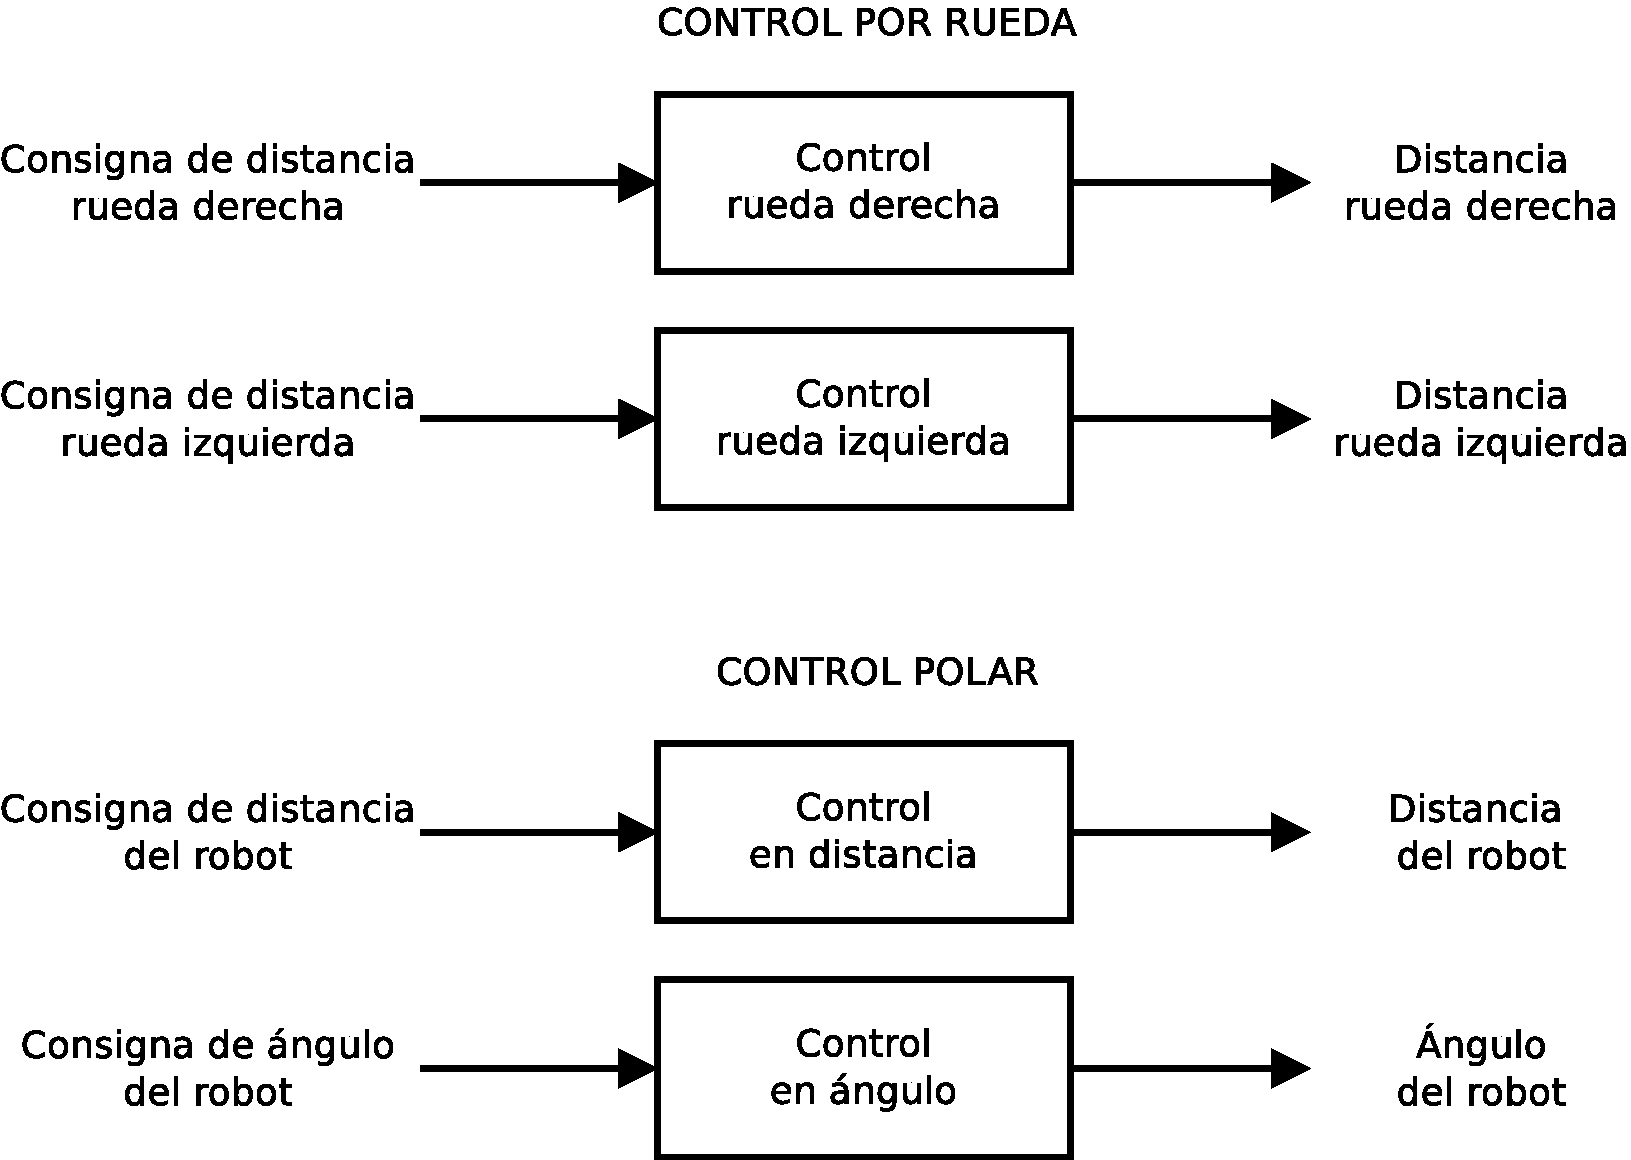
\includegraphics[width=.75\textwidth]{control_polar_vs_por_rueda}
\caption[]{Control de posici�n polar vs. control independiente de posici�n por rueda}
\label{fig_control_polar_vs_por_rueda}
\end{figure}

\begin{figure}[ht]
\centering
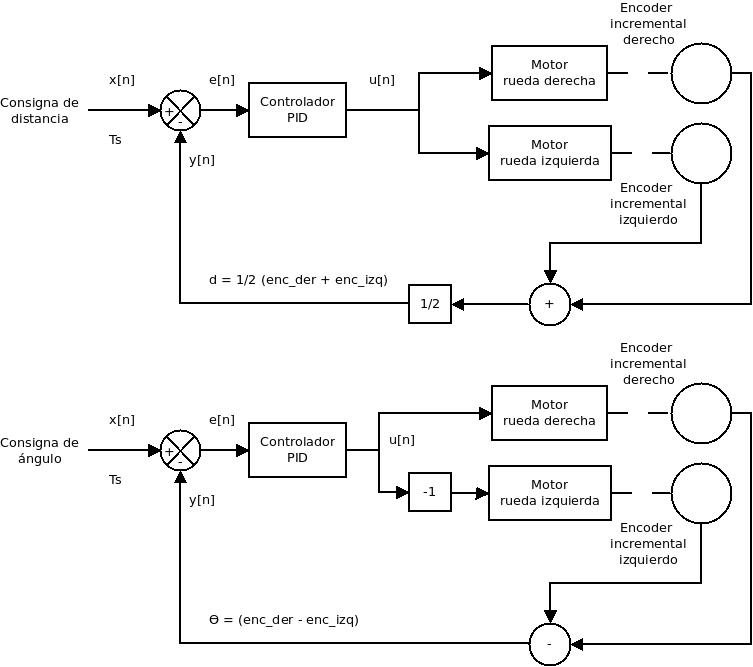
\includegraphics[width=\textwidth]{control_polar}
\caption[]{Diagrama de bloques del control de posici�n polar}
\label{fig_control_polar}
\end{figure}

El diagrama de bloques del controlador polar se muestra en la figura \ref{fig_control_polar}. En cada controlador error de posici�n $e[n]$ se obtiene a partir de la resta de la consigna $x[n]$ y de la medida instant�nea de los encoders $y[n]$ en cada periodo de muestreo $T_s$. Para el caso del control en distancia, $y[n]$ se corresponde con la distancia recorrida por el robot y se obtiene a partir del valor medio de la distancia recorrida por cada encoder. Mientras que en el caso del controlador en �ngulo, $y[n]$ se corresponde con el �ngulo instant�neo del robot y se obtiene a partir de la diferencia de la distancia recorrida por los encoders.

El error de consigna es procesado por un controlador PID (Proporcional Integral Derivativo) generando a su salida la se�al de control $u[n$] para los motores. Notar que en el caso del controlador de distancia la se�al de control es la misma para ambos motores, mientras que en el caso del controlador de �ngulo, el signo de la se�al de control del motor izquierdo se encuentra invertida.

En la practica, se ha utilizado un controlador PD frente al cl�sico PID, esta elecci�n viene dada por el balance entre las ventajas e inconvenientes del termino integral.

Ventajas:
\begin{itemize}
\item Mejor precisi�n en r�gimen permanente
\item Mejor respuesta a perturbaciones
\end{itemize}

Desventajas:
\begin{itemize}
\item Tendencia a desestabilizar el bucle de control
\item Introduce el fen�meno de \emph{windup}\footnote{Efecto por el cual el controlador puede saturarse dando como resultado respuestas bruscas no lineales en el momento que la perturbaci�n cesa}.
\end{itemize}

El termino integral suele ser utilizado en procesos industriales donde la respuesta a perturbaciones es muy importante. Sin embargo, para un robot de Eurobot su uso puede ser cuestionable tal y como se argumenta en \cite{rcva_10x}. Esto es debido a las posibles reacciones bruscas del efecto \emph{windup} y a que en Eurobot una perturbaci�n significa que el robot se ha bloqueado debido a que ha chocado con un oponente o una pared. En dicho caso, si la reductora del robot se ha dimensionado correctamente, las ruedas derraparan, por lo que el termino integral no tendr� ning�n efecto.

Al utilizar una arquitectura PD el sistema de control es tipo 1 \cite{ogata2010}. Por un lado, esto implica que un ajuste m�s sencillo de los controladores. Hay que tener en cuenta que un controlador tipo 1 siempre tendr� un mejor rendimiento y fiabilidad que un controlador tipo 2 mal ajustado. Por otro lado, un sistema de control de tipo 1 implica un error de posici�n nulo ante una entrada tipo escal�n y un error de velocidad constante ante una entrada tipo rampa. Teniendo en cuenta que las consignas de los controladores de posici�n vendr�n dadas a partir de perfiles de velocidad trapezoidal, durante las fases de aceleraci�n y frenado el controlador seguir� a la consigna a la misma velocidad pero con un retardo constante, mientras que durante la fase de velocidad constante o en estado de reposo (robot parado) el error de posici�n ser� nulo. Dado que es en distancia donde se requiere un control preciso, el retardo en velocidad es un factor asumible.

Respecto a la acci�n derivativa de un controlador PID o PD, esta suele introducir cierto ruido en la se�al de control de los motores $u[n]$ y da como resultado un controlador m�s nervioso. Este ruido puede reducirse mediante un controlador del tipo PI-D \cite{ogata2010} donde la correcci�n derivativa se realiza directamente a partir de la medida de los encoders. Este caso ha sido estudiado en \cite{rcva_10x}, donde se comprueban las ventajas de un controlador P-D frente a una arquitectura cl�sica PD. Efectivamente, la se�al de control $u[n]$ es menos ruidosa y de un valor de pico menor, lo que repercute en un control m�s suave de la velocidad del robot. Adem�s se observa que el error $e[n]$ del controlador P-D es menor que en el PD. Por contra, se observa un retardo mayor en las fases de aceleraci�n y frenado para en controlador P-D, consiguiendo la misma aceleraci�n para ambas arquitecturas.

Otra opci�n para disminuir el efecto del termino integral consiste en asignar un periodo de muestreo para el termino derivativo $T_d$ menor que el periodo de muestreo del bucle $T_s$, de forma que, el el error derivativo quede promediado y se consigua una respuesta m�s suave a la salida del controlador.

\subsection{Implementaci�n del perfil de velocidad trapezoidal}

La implementaci�n del perfil de velocidad trapezoidal se consigue mediante un filtro de consigna previo a la consigna de distancia y �ngulo de los controladores (ver figura \ref{fig_filtro_consigna}). Dado que lo que se quiere limitar es la aceleraci�n y la velocidad con la que varia la consigna de posici�n se necesita de un filtro de segundo orden. Dicho filtro eval�a la primera y segunda derivada de la consigna de posici�n $x[n]$, correspondientes a la aceleraci�n y velocidad m�ximas. En caso de superase alguna de ellas la consigna de posici�n a la salida del filtro $x'[n]$ es limitada al valor de la aceleraci�n o la velocidad m�xima, seg�n aplique.

\begin{figure}[ht]
\centering
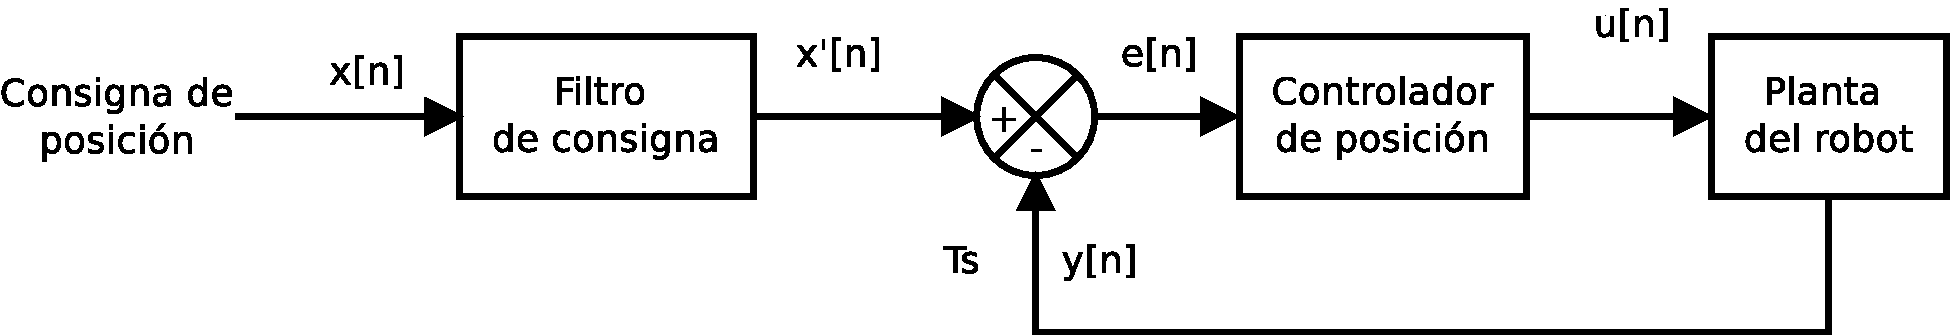
\includegraphics[width=.9\textwidth]{filtro_consigna}
\caption[]{Implementaci�n del perfil de velocidad trapezoidal mediante un filtro de consigna}
\label{fig_filtro_consigna}
\end{figure}


\subsection{Sistema de unidades del robot}

Los controladores de posici�n a implementar trabajan en unidades diferentes a las del sistema internacional (SI). A la hora de establecer la consigna de los mismos o fijar la velocidad y aceleraci�n m�xima del filtro de consigna es necesario conocer los coeficientes de conversi�n entre ambos sistemas de unidades. La tabla \ref{tab_unidades_robot} muestra las unidades de la distancia, velocidad y aceleraci�n para el sistema internacional y el sistema de unidades del robot.

\begin{table}[h]
\centering
\caption{Unidades SI y del sistema robot}
\label{tab_unidades_robot}

\begin{tabular}{ lccc }
\hline
Magnitud	& Simbolo   & Unidades SI 	& Unidades sistema Robot \\
\hline
Distancia 	& $d$ 		& $m$  			& $pulsos$ \\
Velocidad 	& $v$		& $m/s$			& $pulsos/T_s$\\
Aceleraci�n & $a$		& $m/s^2$		& $pulsos/T_s^2$ \\
\hline
\end{tabular}
\end{table}

Los coeficientes de conversi�n de distancia $C_d$, velocidad $C_v$ y aceleraci�n $C_a$ entre sistemas se calculan como:
\begin{align}
C_d &= \frac{N\times M}{\pi\,D_n} \,\Big[\frac{pulsos}{m}\Big] \\
C_v &= C_d\, T_s 				  \,\Big[\frac{pulsos/T_s}{m/s}\Big] \\
C_a &= C_d\, T_s^2  			  \,\Big[\frac{pulsos/T_s^2}{m/s^2}\Big]
\end{align}

Siendo:
\begin{align*}
N &: \text{Numero de pulsos por vuelta de encoder} \\
M &: \text{Factor de multiplicaci�n de decodificaci�n de se�ales en cuadratura del encoder} \\
D_n &: \text{Di�metro nominal del encoder} \\
T_s &: \text{Periodo de muestreo}
\end{align*}

De esta forma dada una distancia $d$, velocidad $v$ y aceleraci�n $a$ en unidades del SI su valor en unidades del robot serian:
\begin{align}
d_r &= C_d\,d \\
v_r &= C_v\,v \\
a_r &= C_a\,a \\
\end{align}

Por ejemplo para los datos, correspondientes al robot P.Tinto (Eurobot 2015):
\begin{align*}
N &= 3600\,pulsos \\
M &= 4 \\
D_n &= 55\,mm \\
T_s &= 5\,ms 
\end{align*}

Se obtienen las constantes
\begin{align*}
C_d &= 83339,121 \\
C_v &= 416,696 \\
C_a &= 2,083
\end{align*}

As� por ejemplo, para una distancia de $1m$, una velocidad de $1m/s$ y una aceleraci�n de $3,6m/s^2$ se obtiene:
\begin{align}
d_r &= C_d\, 1 = 83339,121 \\
v_r &= C_v\, 1 = 416,696 \\
a_r &= C_a\,a 3 = 7,501
\end{align}

Se observa que los valores resultantes son decimales, lo cual implicar�a trabajar con decimales en la implementaci�n de los controladores. Esto no es nada �ptimo desde el punto de vista de procesamiento digital. Una posible soluci�n pasa por redondear dichos valores para poder trabajar con n�meros enteros, pero para valores peque�os como el de la aceleraci�n el error por redondeo podr�a ser considerable. Para solucionar dicha perdida de precisi�n se a�ade un factor $K_{imp}$:
\begin{align}
C_d &= K_{imp}\,\frac{N\times M}{\pi\,D_n} \,\Big[\frac{pulsos}{m}\Big] \\
C_v &= K_{imp}\,C_d\, T_s 				  \,\Big[\frac{pulsos/T_s}{m/s}\Big] \\
C_a &= K_{imp}\,C_d\, T_s^2  			  \,\Big[\frac{pulsos/T_s^2}{m/s^2}\Big]
\end{align}

Por ejemplo, para un $K_{imp}=10$ el valor de la consigna de aceleraci�n seria $a_r=75$ lo que equivale a un error menor del 1\%.

Para que la conversi�n sea v�lida, el factor $K_{imp}$ ha de integrarse en el controlador. Como muestra la figura \ref{fig_control_polar_kimp}, la integraci�n se realiza en el lazo de realimentaci�n de forma que el factor $K_{imp}$ multiplica a la medida de posici�n de los encoders. Notar que la constante $K_{imp}$ no tiene efecto sobre la medida de angulo.

\begin{figure}[ht]
\centering
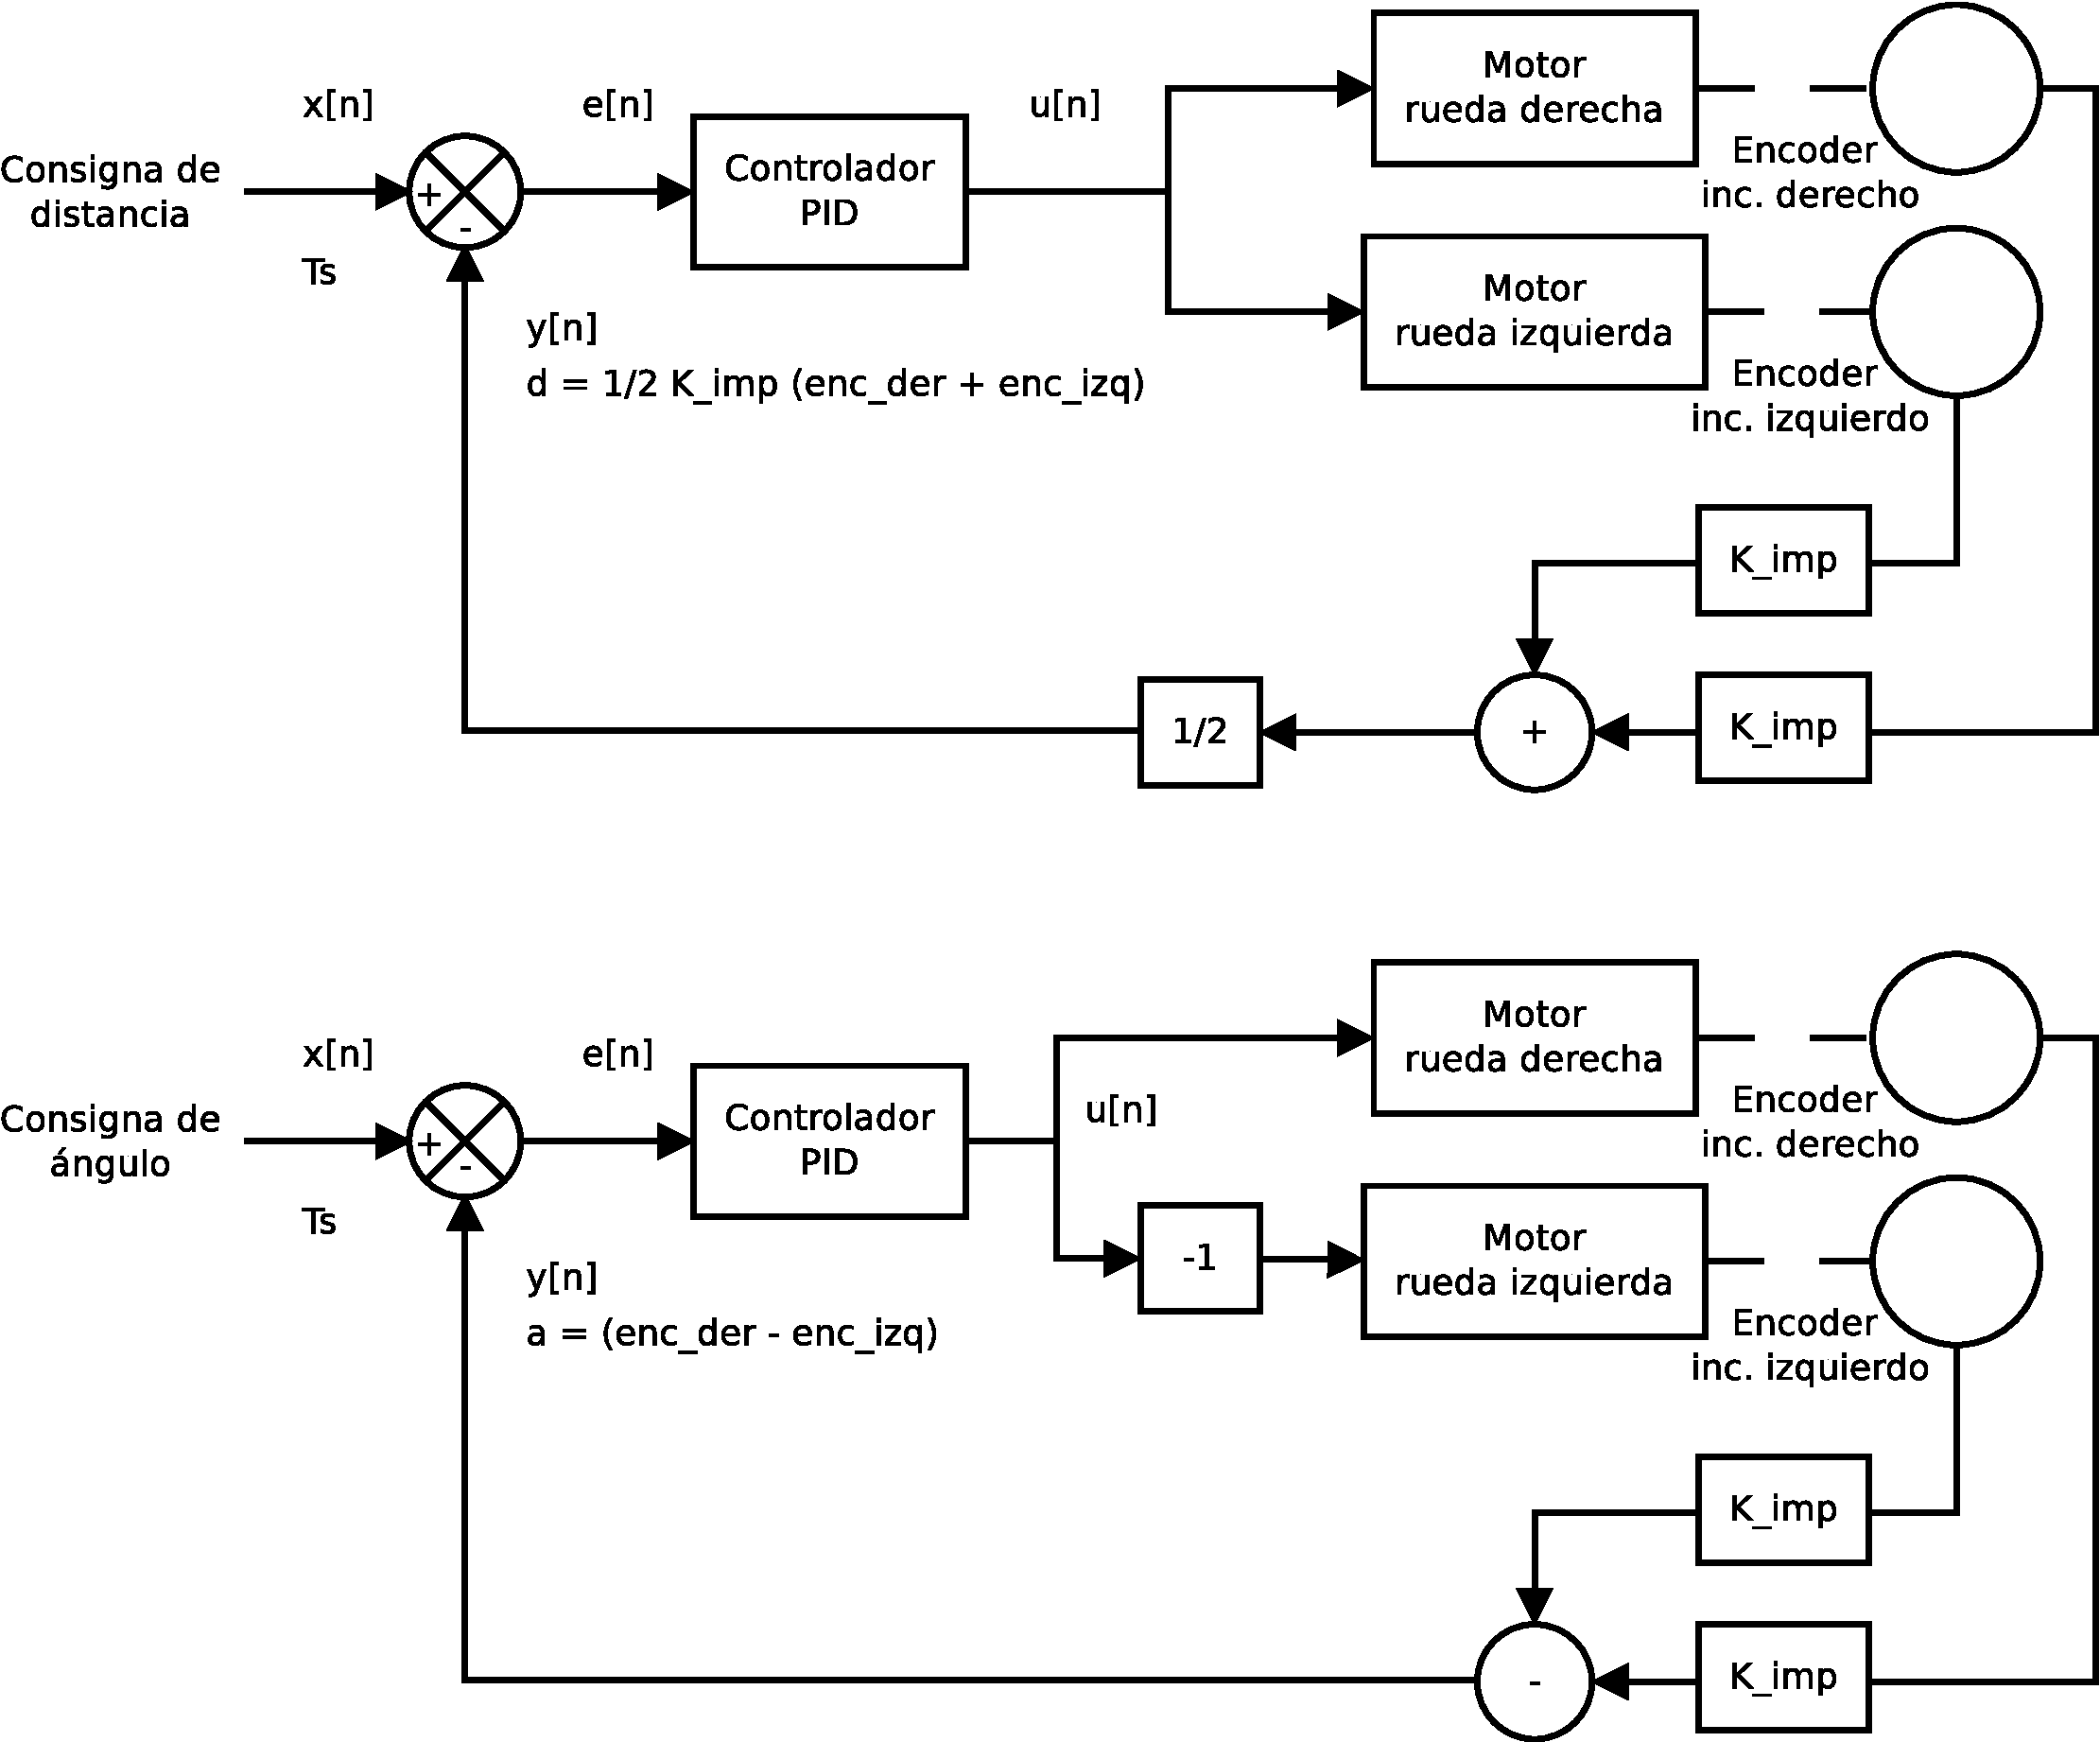
\includegraphics[width=\textwidth]{control_polar_kimp}
\caption[]{Integraci�n del factor $K_{imp}$ en el diagrama de bloques del control de posici�n polar}
\label{fig_control_polar_kimp}
\end{figure}

\subsection{Ajuste del controlador de posici�n}

El m�todo de ajuste utilizado es experimental, al igual que otros m�todos experimentales como los basados en las reglas de Ziegler-Nichols \cite{ogata2010}, permiten obtener una estimaci�n razonable de los par�metros del controlador y proporcionan un punto de partida para una sinton�a fina. 

Independientemente del m�todo utilizado, para conseguir un ajuste preciso de los controladores es indispensable contar con una herramienta de depuraci�n que permita adquirir las diferentes se�ales del diagrama de control y poder representarlas. Por ejemplo, la plataforma desarrollada cuenta con una interfaz serie RS-232 por la cual se vuelcan los datos durante el proceso de ajuste de los controladores.

El proceso de ajuste utilizado es el propuesto en \cite{rcva_10x}. A la hora de llevarlo a cabo es aconsejable primero en ajustar el controlador de �ngulo y posteriormente el de distancia. Esto es debido a que durante el proceso de ajuste del controlador de �ngulo se llevan a cabo ciertas secuencias de rotaci�n, que luego son secuencias de desplazamiento en el caso del controlador de distancia. Si en este �ltimo caso el controlador de �ngulo no est� previamente ajustado, durante el proceso de ajuste del controlador de distancia habr� desviaciones laterales que dificultar�an el proceso.

Primero para ajustar el controlador de �ngulo se bloquea el controlador de distancia fijando una consigna de valor 0. Y luego, para ajustar el controlador de distancia se hace lo contrario, y se fija una consigna de �ngulo igual a 0. El ajuste de ambos controladores se hace sin ning�n tipo de perfil o rampa de velocidad, se busca observar la respuesta a una perturbaci�n tipo escal�n. 

Para cada controlador se ajusta primero el termino proporcional, luego el termino derivativo y por �ltimo, si corresponde, el termino integral. En este caso se presenta el proceso de ajuste de un controlador PD.

\begin{enumerate}
\item Ajuste del termino proporcional $K_p$:
	\begin{enumerate}
	\item Anular la correcci�n derivativa $K_d=0$.
	\item Fijar una ganancia $K_p$ inicial.
	\item Saca al controlador de su posici�n de equilibrio. Desplazamientos entre 5 y 10 grados en �ngulo, o $5cm$ en distancia.
	\item Observar las gr�ficas de la respuesta del controlador.
	\item Incrementar el valor de $K_p$ hasta observar en las gr�ficas una respuesta amortiguada de duraci�n entre 1 y 2 segundos.
	\end{enumerate}

\item Ajuste del termino derivativo $K_d$:
	\begin{enumerate}
	\item Fijar una ganancia $K_d$ inicial.
	\item Saca al controlador de su posici�n de equilibrio. Desplazamientos entre 5 y 10 grados en �ngulo, o $5cm$ en distancia.
	\item Observar las gr�ficas de la respuesta del controlador.
	\item Incrementar el valor de $K_d$ hasta observar en las gr�ficas que se obtiene una respuesta sin oscilaciones amortiguadas correspondiente hasta llegar una respuesta subamortiguada con un sobreimpulso $M_p$ cercano al $4.6\%$ ($\xi=0,7$).
	\end{enumerate}
\end{enumerate}

La figuras \ref{fig_ajuste_kp_figure_2} y \ref{fig_ajuste_kd_figure_2} muestra las gr�ficas obtenidas una vez realizado el ajuste de los t�rminos del controlador de distancia.

Una vez ajustados ambos controladores es posible realizar un ajuste fino de los mismos con el fin de obtener un tiempo de establecimiento. Siguiendo el mismo procedimiento descrito para el ajuste, se incrementa el termino $K_p$ en un 20\% y se vuelve a ajustar el termino derivativo. Se repite esta operaci�n sucesivamente hasta el momento en el que el termino $K_d$ no sea capaz de compensar el incremento de $K_p$ poniendo atenci�n en que la se�al de control del motor $u[n]$ no sature.

\begin{figure}[ht]
\centering
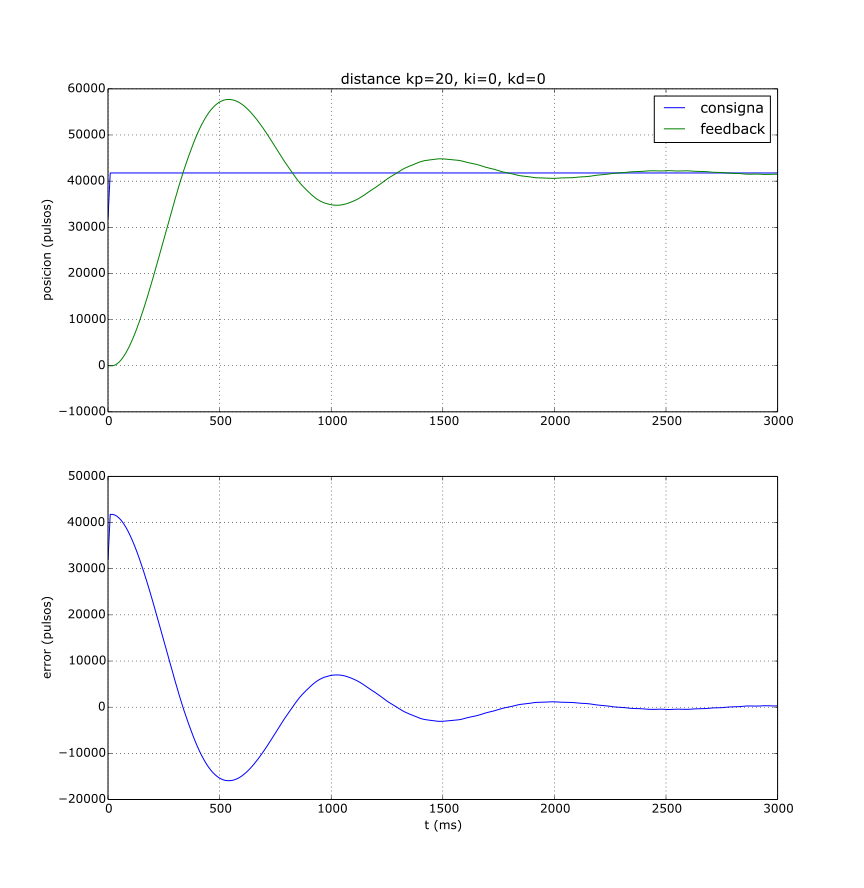
\includegraphics[width=.9\textwidth]{ajuste_kp_figure_2}
\caption[]{Resultado del ajuste del termino proporcional $K_p$ del controlador de distancia ante una consigna tipo escal�n de $5cm$}
\label{fig_ajuste_kp_figure_2}
\end{figure}

\begin{figure}[ht]
\centering
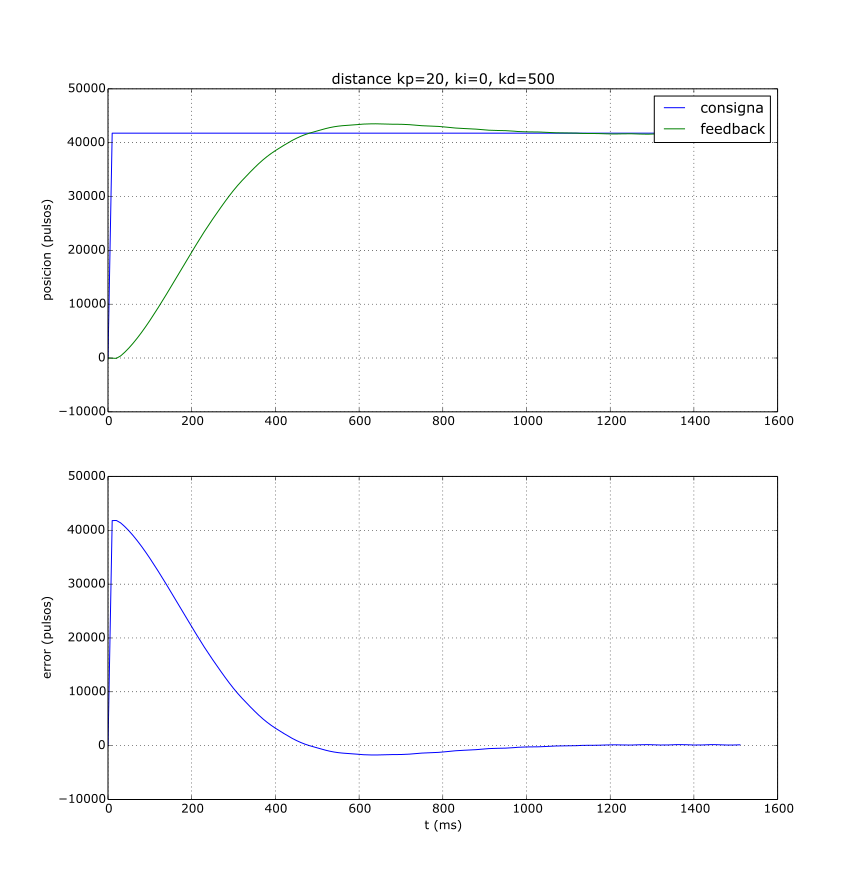
\includegraphics[width=.9\textwidth]{ajuste_kd_figure_2}
\caption[]{Resultado del ajuste del termino proporcional $K_d$ del controlador de distancia ante una consigna tipo escal�n de $5cm$}
\label{fig_ajuste_kd_figure_2}
\end{figure}


Por �ltimo, se realiza un �ltimo ajuste de los controladores a aplicando la consigna dada por el perfil de velocidad trapezoidal. En este �ltimo ajuste se busca obtener una fase de aceleraci�n y frenado �ptimo. Para ello se ha de prestar atenci�n en que durante y al final de cada una de estas fase no existan variaciones bruscas de la posici�n del robot que puedan causar sobre impulsos de aceleraci�n superiores a la aceleraci�n m�xima. Esto es, que la posici�n se ci�a a la forma del perfil lo m�ximo posible. En las figuras \ref{fig_ajuste_perfil_1} y \ref{fig_ajuste_perfil_2} se muestra el resultado de ajustar el controlador de distancia con un perfil trapezoidal.


\begin{figure}[p]
\centering
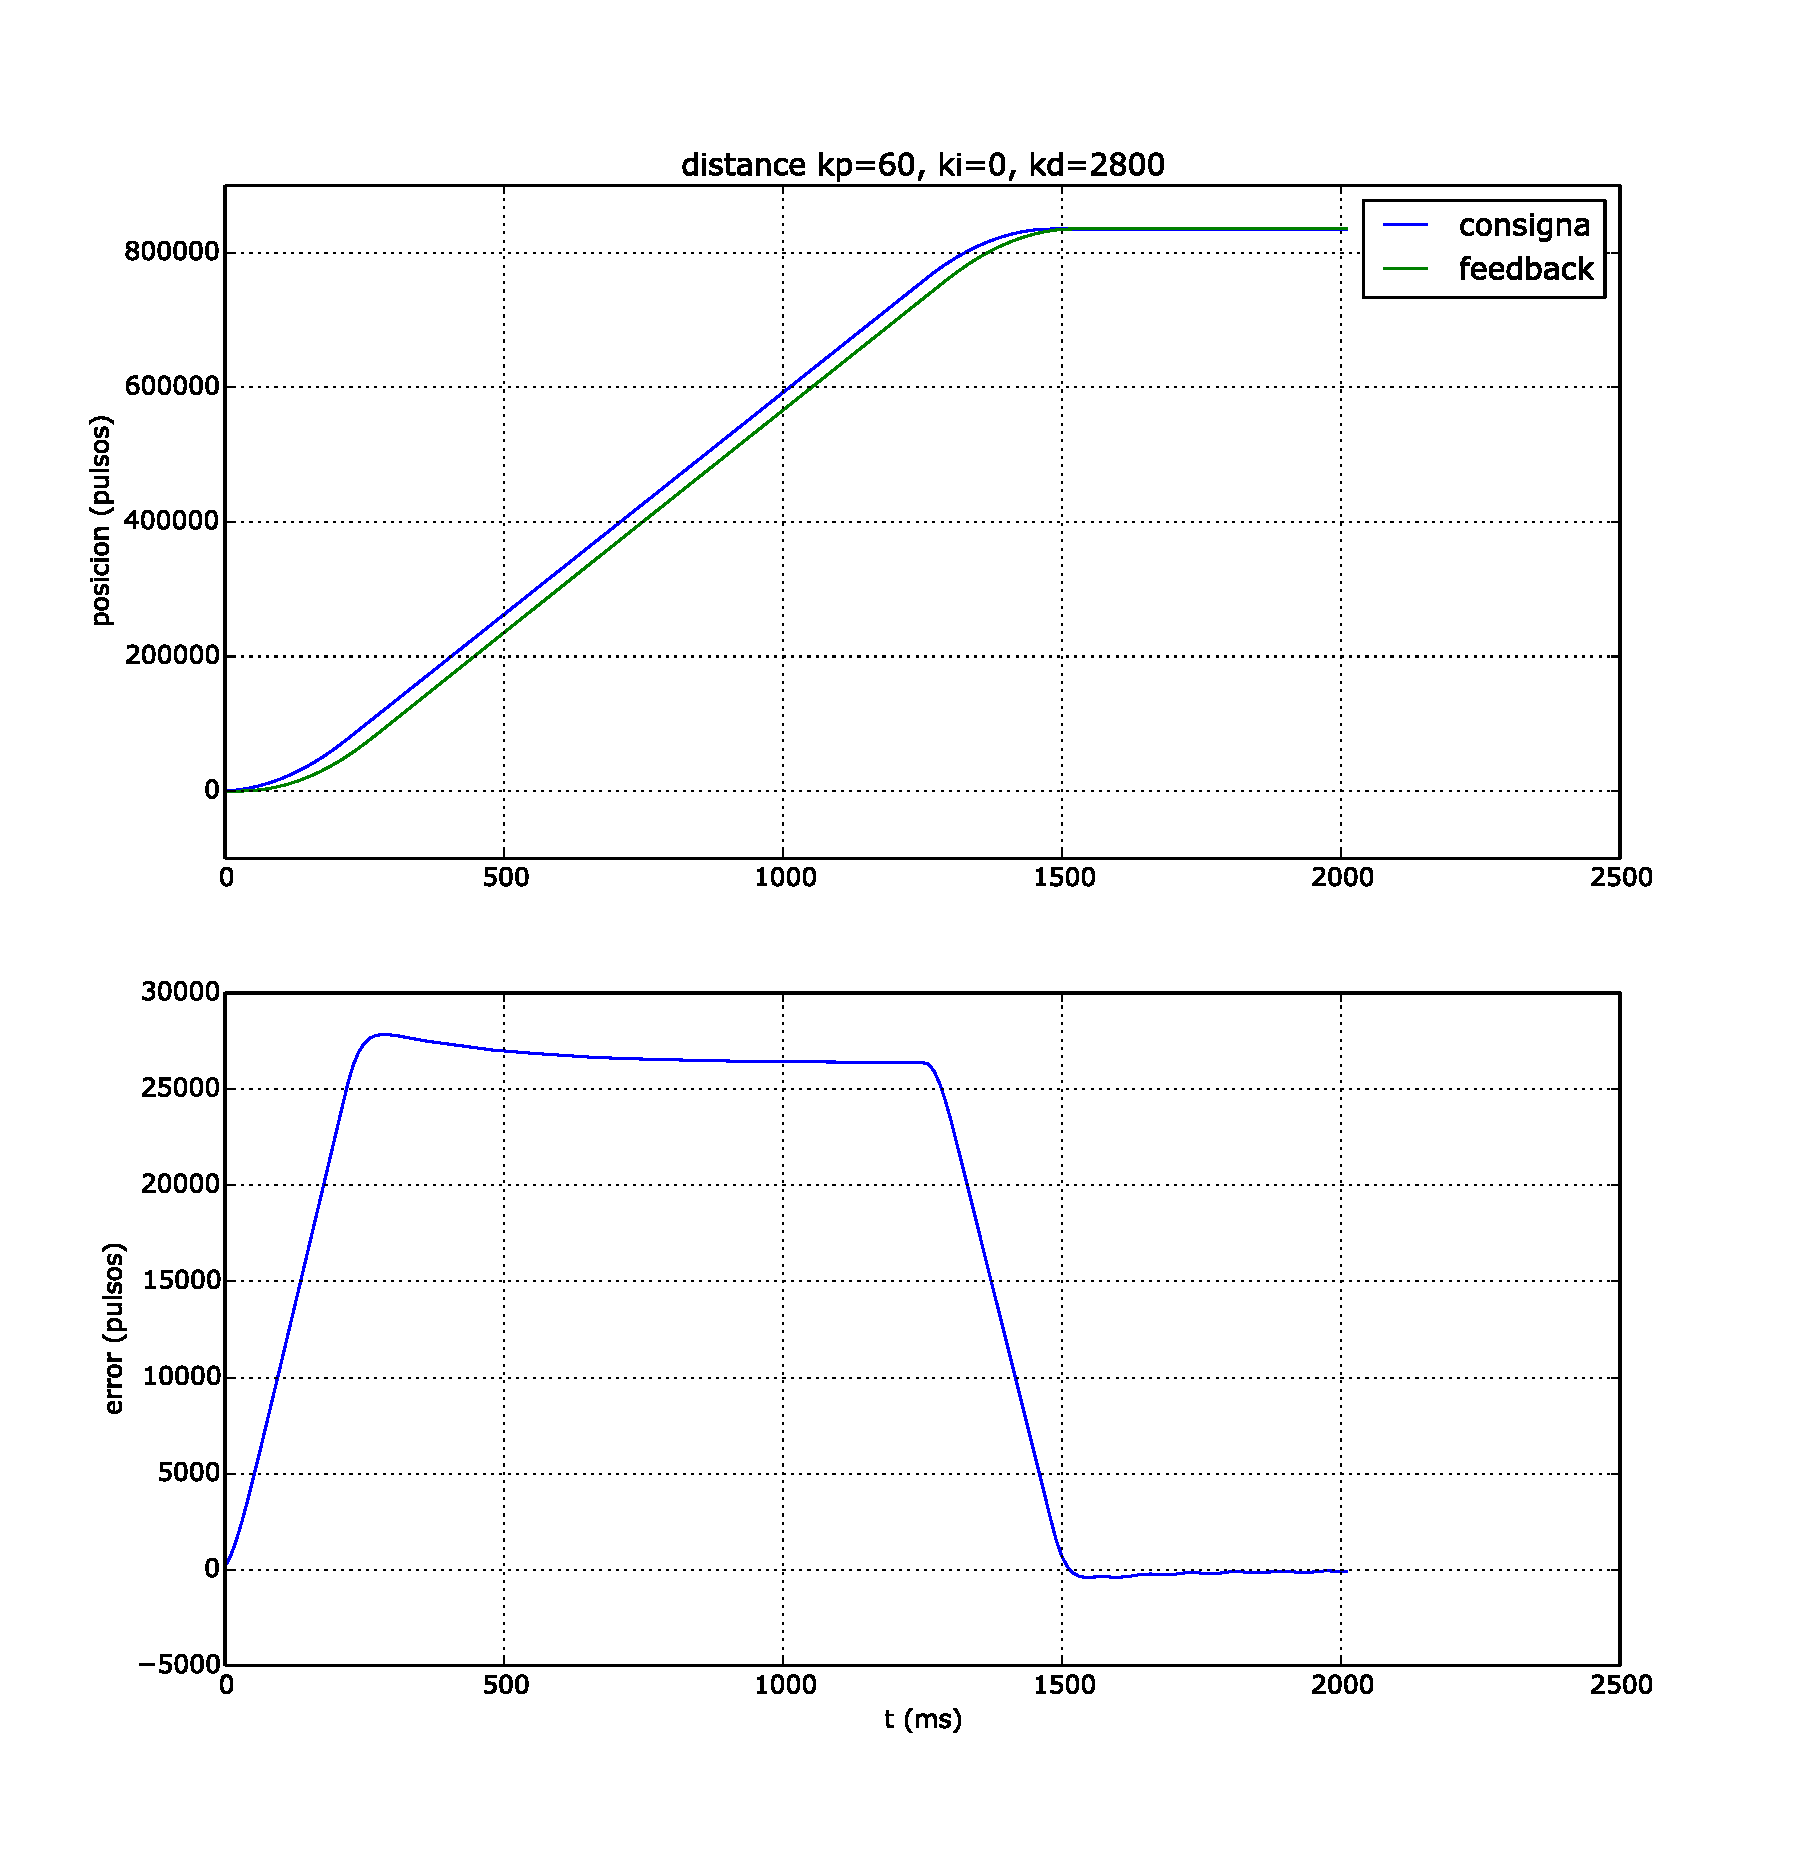
\includegraphics[width=\textwidth]{ajuste_kp_kd_perfil_figure_2}
\caption[]{Resultado del ajuste del controlador de distancia aplicando un perfil de velocidad trapezoidal ($a=3,45m/s^2$, $v=0,8m/s$).}
\label{fig_ajuste_perfil_1}
\end{figure}

\begin{figure}[p]
\centering
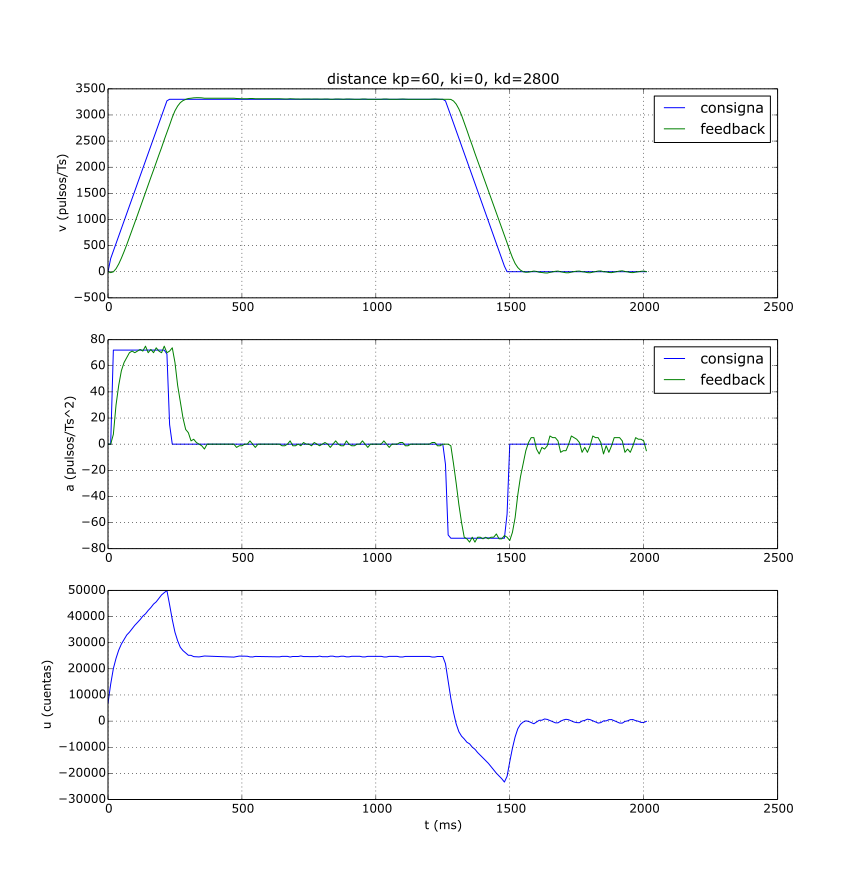
\includegraphics[width=\textwidth]{ajuste_kp_kd_perfil_figure_1}
\caption[]{Resultado del ajuste del controlador de distancia aplicando un perfil de velocidad trapezoidal ($a=3,45m/s^2$, $v=0,8m/s$)}
\label{fig_ajuste_perfil_2}
\end{figure}

% TODO someday
%\subsection{Compensaci�n de la gravedad}
%\subsection{Estimaci�n de bloqueos mec�nicos en el lazo de controlador}

\pagebreak
\section{Posicionamiento mediante odometr�a}

La odometr�a es el m�todo m�s usado para determinar la posici�n moment�nea de un robot. Dicha posici�n viene dada en un plano cartesiano por sus coordenadas absolutas $(x,y,\theta)$ correspondientes a la distancia al origen de coordenadas y al �ngulo respecto al eje de abscisas. 

\subsection{Calculo de la posici�n del robot}

El sistema desarrollado para implementar este tipo de posicionamiento es el sistema de ruedas libres descrito en la secci�n \ref{sec_sma_posicionamiento_y_control}. Los principales elementos de este sistema y las dimensiones relacionada con la implementaci�n de este m�todo se muestra en la figura \ref{fig_odometria_dimensiones} donde $D_n$ se corresponden con el di�metro nominal de las ruedas de los encoders y $b$ con la distancia entre ejes de rueda de encoder.

\begin{figure}[ht]
\centering
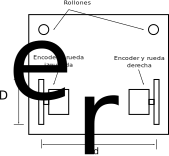
\includegraphics[width=.4\textwidth]{odometria_dimensiones}
\caption[]{Representaci�n en planta del robot. Componentes y dimensiones implicas en la odometr�a}
\label{fig_odometria_dimensiones}
\end{figure}

La determinaci�n de la posici�n $(x,y,\theta)$ del robot se obtiene a partir la medida del incremento de pulsos de cada encoder por periodo de muestreo $Ts$. A partir de la medida en un periodos de muestreo de los pulsos del encoder derecho $N_D$ e izquierdo $N_I$ se obtiene la medida de instant�nea de distancia $d$ y �ngulo $\theta$ en cada periodo de muestreo como:

\begin{align}
d = \frac{N_D + N_I}{2}\, [pulsos] \label{eq_d_pulsos}\\
\theta = (N_D - N_I)\, [pulsos] \label{eq_angle_pulsos}
\end{align}

La conversi�n de unidades del robot a unidade del SI se realiza multiplicando dichas medidas por los factores de conversi�n de distancia $C_d$ y angulo $C_\theta$, calculados como:

\begin{align}
C_d &= \frac{N\times M}{\pi\,D_n} \,\Big[\frac{pulsos}{m}\Big] \label{eq_coef_d}\\
C_\theta &= C_d\,\frac{b}{2} \Big[\frac{pulsos}{rad}\Big] \label{eq_coef_angle}
\end{align}

Por un lado, la coordenada $\theta$ del robot puede obtenerse directamente de la equaci�n \eqref{eq_angle_pulsos} como:

\begin{align}
\boxed{\theta_n = \frac{N_{D\,n} - N_{I\,n}}{C_\theta} [rad]} \label{eq_angle_rad}
\end{align}


Por otro lado, las coordenadas $(x,y)$ se calculan a partir del analisis de la trayectoria del robot muestreada para dos instantes consecutivos (ver figura \ref{fig_odometria_geometria}). Las posiciones A y B se corresponden con los instantes $n$ y $n-1$ a los que les corresponde una medida de angulo $\theta_n$ y $\theta_{n-1}$ y una medida de distancia $d_n$ y $d_{n-1}$. La distancia curvil�nea entre los puntos A y B es $L$ y su proyecci�n sobre los ejes $dx$ y $dy$. 

\begin{figure}[ht]
\centering
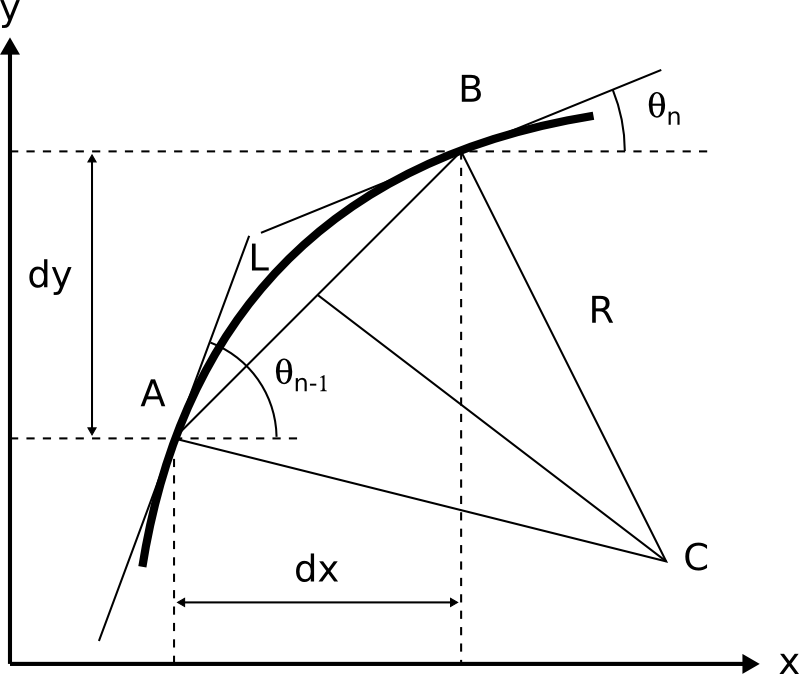
\includegraphics[width=.5\textwidth]{odometria_geometria}
\caption[]{Representaci�n geom�trica de dos puntos de una trayectoria}
\label{fig_odometria_geometria}
\end{figure}

Las coordenadas $(x,y)$ en un instante dado se corresponden con:

\begin{align}
x_n &= x_{n-1} + dx \\
y_n &= y_{n-1} + dy \\
\end{align}

En teor�a la obtenci�n de las proyecciones $dx$ y $dy$ resulta imposible dado que se desconoce la forma de la trayectoria $L$ descrita entre los dos instantes de muestreo. En la pr�ctica se aplica una aproximaci�n lineal o circular, de forma que $L$ se aproxima a una recta o a un arco de circunferencia de radio $R$ y centro de giro en $C$.

Para el caso de la aproximaci�n lineal el �ngulo del segmento AB $\theta_{avg}$ se calcula como el valor medio del �ngulo en cada punto:

\begin{equation}
\theta_{avg} = \frac{\theta_n + \theta_{n-1}}{2}
\end{equation}

Por la aproximaci�n lineal, $L$ se corresponde con la longitud del segmento AB:
\begin{equation}
L = d_n - d_{n-1}
\end{equation}

El valor de $dx$ y $dy$ para la aproximaci�n lineal se obtiene como:

\begin{empheq}[box=\fbox]{align}
dx &= L\,\cos(\theta_{avg})\\
dy &= L\,\sin(\theta_{avg})
\end{empheq}

El calculo de odometr�a utilizando la aproximaci�n circular se resuelve en \cite{rcva_odometri}. Para dicha aproximaci�n el valor de $dx$ y $dy$ se obtiene como:

\begin{empheq}[box=\fbox]{align}
dx &= K\,L\,\cos(\theta_{avg})\\
dy &= K\,L\,\sin(\theta_{avg})
\end{empheq}

Siendo  
\begin{align}
K &= \frac{\sin(\nabla\theta_n/2)}{\nabla\theta_n/2} \\
\nabla \theta_n &= \theta_n - \theta_{n-1}
\end{align}

Observar que las expresiones de ambas aproximaciones difieren �nicamente en el factor $K$ que constituye un factor de escala para $L$. El estudio comparativo entre ambas aproximaciones realizada en \cite{rcva_odometri} demuestra que para las condiciones de un robot de Eurobot la aproximaci�n circular no a�ade ninguna ventaja frente a la aproximaci�n lineal. En la aproximaci�n circular, adem�s de necesitar mayor tiempo de calculo, la correcci�n aportada por $K$ para trayectorias muy exigentes se encuentra en $1\times10^{-5}$ y $2\times10^{-5}$, algo despreciable.



\subsection{Medida y correcci�n de errores sistem�ticos}

El principal inconveniente de la odometr�a es la acumulaci�n continua de error a medida que el robot se desplaza. Estos errores pueden sistem�ticos y no sistem�ticos. 

\begin{description}
\item Errores sistem�ticos
\begin{enumerate}
\item Diferente di�metro de las ruedas de encoder.
\item Valor medio del di�metro de las ruedas de encoder diferente del di�metro nominal.
\item Ruedas de encoder desalineadas.
\item Incertidumbre en la distancia efectiva entre ejes de las ruedas de encoder o de tracci�n (debido al punto de apoyo con el suelo).
\item Resoluci�n del encoder insuficiente
\item Tiempo de muestreo limitado
\end{enumerate}

\item Errores no sistem�ticos
\begin{enumerate}
\item Trayectos sobre suelos irregulares
\item Trayectos sobre objetos inesperados en el suelo
\item Deslizamiento de las ruedas de encoder debido a: sobre-aceleraciones, suelos resbaladizos, fuerzas externas (colisi�n con robot oponente), fuerzas internas (bloqueo de los rollones) o falta de contacto de as ruedas con el suelo.
\end{enumerate}
\end{description}

Los errores sistem�ticos son particularmente graves debido a que se acumulan constantemente, incluso llegan a contribuir al error m�s que los errores no sistem�ticos. En el caso de superficies irregulares los errores no sistem�ticos podr�an contribuir m�s, pero no es el caso de los robots Eurobot donde las superficies son lisas. Adem�s, el sistema de ruedas libres de la plataforma rob�tica permite evitar los errores no sistem�ticos debido al deslizamiento de las ruedas.

Respecto a los errores sistem�ticos, las ecuaciones de calculo de la odometr�a pueden introducir errores debido a la aproximaci�n  del m�todo utilizado en su calculo. La precisi�n en dicho calculo depende del tiempo de muestreo frente a la velocidad del robot. Este error puede considerarse despreciable si se trabaja con periodos de muestreo de $T_s<10\,ms$ para velocidades de $v < 1\,m/s$ \cite{bor96_ieeet}.

Los errores sistem�ticos no suelen cambiar durante el recorrido del robot, aunque la distribuci�n de pesos sobre las ruedas de encoders puede afectar si estas se encuentra solidarias a la estructura del robot. No es el caso del sistema de ruedas libre desarrollado en el que estas se encuentra desacopladas mediante un mecanismo lineal o pivotante con amortiguaci�n.

Los errores sistem�ticos son normalmente causados por imperfecciones en la implementaci�n del dise�o y la mec�nica del robot. Las dos fuentes de errores sistem�ticos m�s significativas son la diferencia de di�metros de rueda de encoder y la incertidumbre en la distancia efectiva entre ejes de las ruedas de encoder o de tracci�n.

El error por diferente di�metro de rueda de encoder se representa por $E_d$  y se define como

\begin{equation}
E_d = \frac{D_R}{D_L}
\end{equation}

donde $D_R$ y $D_L$ son los di�metros reales de las ruedas de los encoders, siendo la relaci�n nominal entre di�metro de ruedas $1.0$.

Como se ha visto en la ecuaci�n \eqref{eq_coef_angle} la medida de �ngulo del robot depende de la distancia entre ejes de ruedas de encoder $b$. Por lo tanto una incertidumbre en dicha distancia implica un error en el calculo. Este error se denota como $E_b$ y se define como

\begin{equation}
E_b = \frac{b_{real}}{b_{nominal}}
\end{equation}

donde $b$ es la distancia entre ejes de ruedas de encoder.



 
El di�metro real de la ruedas es al angulo real de giro como el diamtro nominal de la rueda al �ngulo de giro.

Conclusiones.

- Diametros distintos de rueda no causan un error de orientaci�n durante los giros.
- El error de orientaci�n depende del di�metro medio de las ruedas

$D_{avg} = \frac{D_L+D_R}{2}$

Si $D_{avg} > D_n$ el robot girar� m�s de lo deseado. Si $D_{avg} < D_n$ entonces el robot girar� menos.

- $E_d$ tiene un efecto menor en la posici�n $x$ e $y$ del centro de giro $C$ porque el centro de rotaci�n real $C'$ no coincide con $C'$, como muestra la figura \ref{}.

Seg�n \cite{} si se quiere reducir los errores de odometr�a, los errores de �ngulo son la principal preocupaci�n ya que una vez se incurre en ellos crecen sin l�mite. 



\begin{figure}[ht]
\centering
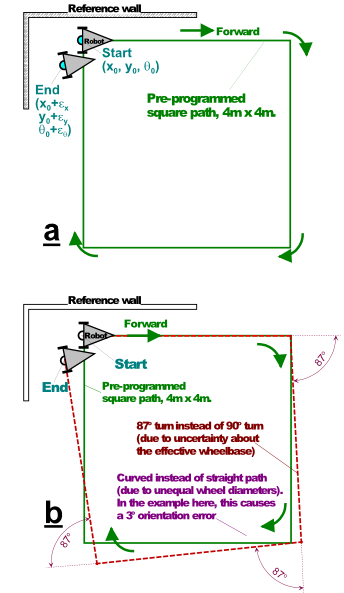
\includegraphics[width=.5\textwidth]{paper58_square_test}
\caption[]{}
\label{fig_paper58_square_test}
\end{figure}

\begin{figure}[ht]
\centering
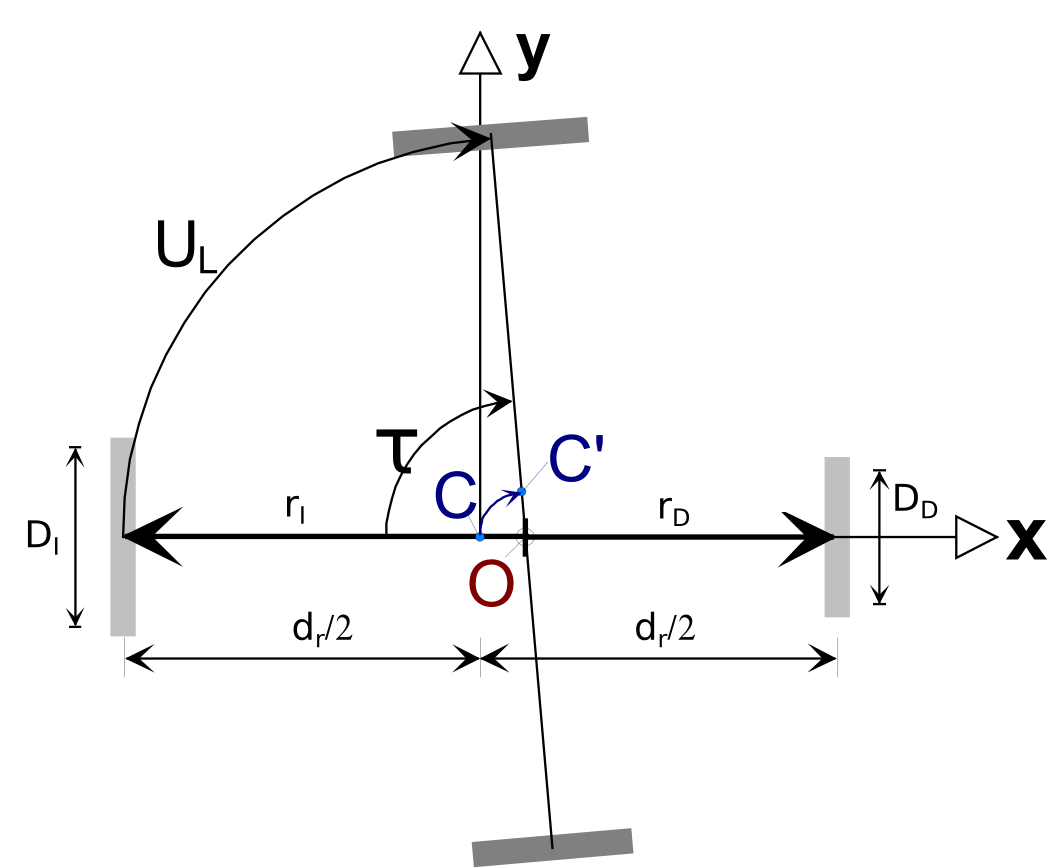
\includegraphics[width=.5\textwidth]{paper58_errores_giro}
\caption[]{}
\label{fig_paper58_errores_giro}
\end{figure}

\begin{figure}[ht]
\centering
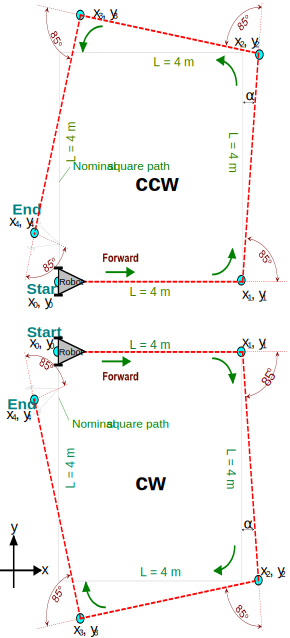
\includegraphics[width=.5\textwidth]{paper58_error_tipo_a}
\includegraphics[width=.5\textwidth]{paper58_error_tipo_b}
\caption[]{}
\label{fig_paper58_}
\end{figure}

\begin{figure}[ht]
\centering
\includegraphics[width=.5\textwidth]{paper58_combinacion_errores}
\caption[]{}
\label{fig_paper58_combinacion_errores}
\end{figure}

\begin{figure}[ht]
\centering
\includegraphics[width=.5\textwidth]{paper58_compensacion_errores}
\caption[]{}
\label{fig_paper58_compensacion_errores}
\end{figure}


\begin{figure}[ht]
\centering
\includegraphics[width=.8\textwidth]{odometria_correccion_error_tipo_a}
\caption[]{}
\label{fig_odometria_correccion_error_tipo_a}
\end{figure}

\begin{figure}[ht]
\centering
\includegraphics[width=.8\textwidth]{odometria_correccion_error_tipo_b}
\caption[]{}
\label{fig_odometria_correccion_error_tipo_b}
\end{figure}

% TODO
%\subsection{Compensaci�n de la fuerza centr�peta}







%%% Local Variables:
%%% TeX-master: "../book"
%%% End:



\chapter{Sistemas mec�nicos para la manipulaci�n de elementos de juego}
\section{Introducci�n}
\section{Soluciones mec�nicas conocidas}
	\subsection{An�lisis de mecanismos utilizados seg�n los elementos de juego}
	\subsection{Conclusiones en la elecci�n de un sistema mec�nico}

\section{Partes de un sistema mec�nico}

\section{Lectura y procesamiento de sensores}
	\subsection{Tipos de sensores}
	\subsection{Electr�nica de acondicionamiento}
	\subsection{Filtrado de sensores digitales}
	\subsection{Filtrado de sensores anal�gicos}

\section{Control de actuadores}
	\subsection{Tipos de actuadores}
	\subsection{Electr�nica de control}

\section{Control de mecanismos}
\section{Sincronizaci�n de sistemas mecanismos y movimiento del robot}




\chapter{Implementaci�n de la estrategia de juego}

\section{Introducci�n}
\begin{itemize}
\item Union de la plataforma rob�tica y los sistemas mec�nicos.
\end{itemize}

\section{Elementos y fases de un partido de Eurobot}

	\begin{itemize}
	\item Patron implicito: recolectar, transportar y almacenar/construir.
	\item Dependencias entre capacidad de recolectar y numero de veces que se almacena
	\item Tipos de tareas: de accion, de recolectar, transportar y almacenar
	\item Tipos de trayectorias en funci�n del campo de juego (caminos libres vs preestablecidos)
	\item{Independencia de los sistemas mec�nicos y las trayectorias}
	\item{Modularidad y flexibilidad de la estrategia}
	\end{itemize}

	\subsection{Zonas de trabajo}
	\subsection{Tareas de una zona de trabajo}
	\subsection{Trayectorias entre zonas de trabajo}
	\subsection{Condiciones en la elecci�n de una zona de trabajo}

\section{Arquitectura software}

\section{Gestion de trayectorias en un partido}
\begin{itemize}
\item Sobrecarga de las trajectorias del sistema base.
\end{itemize}

\section{Comunicaci�n entre dos robots}

\section{Simulaci�n de estrategias}

\section{Patrones de implementaci�n de estrategia}
	\subsection{Estrategia secuencial bloqueante}
	\subsection{Estrategia reactiva}
	\subsection{Estrat�gia basada en prioridades}
	\subsection{Estrat�gia adaptativa}
	\subsection{Estrategia con dos robots}

\section{Pruebas, depuraci�n y validaci�n de la estrategia}



% Optional in PFCs
%%%%%%%%%%%%%%%%%%%%%%%%%%%%%%%%%%%%%%%%%%%%%%%%%%%%%%%%%%%%%%%%%%%%%%%%%%%%
%
% Generic template for TFC/TFM/TFG/Tesis
%
% $Id: pliego.tex,v 1.4 2014/01/08 22:56:06 macias Exp $
%
% By:
%  + Javier Mac�as-Guarasa. 
%    Departamento de Electr�nica
%    Universidad de Alcal�
%  + Roberto Barra-Chicote. 
%    Departamento de Ingenier�a Electr�nica
%    Universidad Polit�cnica de Madrid   
% 
% Based on original sources by Roberto Barra, Manuel Oca�a, Jes�s Nuevo,
% Pedro Revenga, Fernando Herr�nz and Noelia Hern�ndez. Thanks a lot to
% all of them, and to the many anonymous contributors found (thanks to
% google) that provided help in setting all this up.
%
% See also the additionalContributors.txt file to check the name of
% additional contributors to this work.
%
% If you think you can add pieces of relevant/useful examples,
% improvements, please contact us at (macias@depeca.uah.es)
%
% Copyleft 2013
%
%%%%%%%%%%%%%%%%%%%%%%%%%%%%%%%%%%%%%%%%%%%%%%%%%%%%%%%%%%%%%%%%%%%%%%%%%%%

\chapter{Pliego de condiciones}
\label{cha:pliego-de-condiciones}

Blah, blah, blah.

%%% Local Variables:
%%% TeX-master: "../book"
%%% End:


% Optional in PFCs, compulsory in TFGs
%%%%%%%%%%%%%%%%%%%%%%%%%%%%%%%%%%%%%%%%%%%%%%%%%%%%%%%%%%%%%%%%%%%%%%%%%%%%
%
% Generic template for TFC/TFM/TFG/Tesis
%
% $Id: presupuesto.tex,v 1.4 2014/01/08 22:56:06 macias Exp $
%
% By:
%  + Javier Mac�as-Guarasa. 
%    Departamento de Electr�nica
%    Universidad de Alcal�
%  + Roberto Barra-Chicote. 
%    Departamento de Ingenier�a Electr�nica
%    Universidad Polit�cnica de Madrid   
% 
% Based on original sources by Roberto Barra, Manuel Oca�a, Jes�s Nuevo,
% Pedro Revenga, Fernando Herr�nz and Noelia Hern�ndez. Thanks a lot to
% all of them, and to the many anonymous contributors found (thanks to
% google) that provided help in setting all this up.
%
% See also the additionalContributors.txt file to check the name of
% additional contributors to this work.
%
% If you think you can add pieces of relevant/useful examples,
% improvements, please contact us at (macias@depeca.uah.es)
%
% Copyleft 2013
%
%%%%%%%%%%%%%%%%%%%%%%%%%%%%%%%%%%%%%%%%%%%%%%%%%%%%%%%%%%%%%%%%%%%%%%%%%%%

\chapter{Presupuesto}
\label{cha:presupuesto}

Blah, blah, blah.

%%% Local Variables:
%%% TeX-master: "../book"
%%% End:


%
% END Normal chapters. Edit/modify all within this section
%%%%%%%%%%%%%%%%%%%%%%%%%%%%%%%%%%%%%%%%%%%%%%%%%%%%%%%%%%%%%%%%%%%%%%%%%%%
%%%%%%%%%%%%%%%%%%%%%%%%%%%%%%%%%%%%%%%%%%%%%%%%%%%%%%%%%%%%%%%%%%%%%%%%%%%
%%%%%%%%%%%%%%%%%%%%%%%%%%%%%%%%%%%%%%%%%%%%%%%%%%%%%%%%%%%%%%%%%%%%%%%%%%%
%%%%%%%%%%%%%%%%%%%%%%%%%%%%%%%%%%%%%%%%%%%%%%%%%%%%%%%%%%%%%%%%%%%%%%%%%%%
%%%%%%%%%%%%%%%%%%%%%%%%%%%%%%%%%%%%%%%%%%%%%%%%%%%%%%%%%%%%%%%%%%%%%%%%%%%
%%%%%%%%%%%%%%%%%%%%%%%%%%%%%%%%%%%%%%%%%%%%%%%%%%%%%%%%%%%%%%%%%%%%%%%%%%%
%%%%%%%%%%%%%%%%%%%%%%%%%%%%%%%%%%%%%%%%%%%%%%%%%%%%%%%%%%%%%%%%%%%%%%%%%%%


%%%%%%%%%%%%%%%%%%%%%%%%%%%%%%%%%%%%%%%%%%%%%%%%%%%%%%%%%%%%%%%%%%%%%%%%%%%
% Bibliography
%%%%%%%%%%%%%%%%%%%%%%%%%%%%%%%%%%%%%%%%%%%%%%%%%%%%%%%%%%%%%%%%%%%%%%%%%%%
%%%%%%%%%%%%%%%%%%%%%%%%%%%%%%%%%%%%%%%%%%%%%%%%%%%%%%%%%%%%%%%%%%%%%%%%%%%
%
% Generic template for TFC/TFM/TFG/Tesis
%
% $Id: bibliography.tex,v 1.7 2014/01/08 22:56:04 macias Exp $
%
% By:
%  + Javier Mac�as-Guarasa. 
%    Departamento de Electr�nica
%    Universidad de Alcal�
%  + Roberto Barra-Chicote. 
%    Departamento de Ingenier�a Electr�nica
%    Universidad Polit�cnica de Madrid   
% 
% Based on original sources by Roberto Barra, Manuel Oca�a, Jes�s Nuevo,
% Pedro Revenga, Fernando Herr�nz and Noelia Hern�ndez. Thanks a lot to
% all of them, and to the many anonymous contributors found (thanks to
% google) that provided help in setting all this up.
%
% See also the additionalContributors.txt file to check the name of
% additional contributors to this work.
%
% If you think you can add pieces of relevant/useful examples,
% improvements, please contact us at (macias@depeca.uah.es)
%
% Copyleft 2013
%
%%%%%%%%%%%%%%%%%%%%%%%%%%%%%%%%%%%%%%%%%%%%%%%%%%%%%%%%%%%%%%%%%%%%%%%%%%%

%\bibliographystyle{plainnat}
%\bibliographystyle{dinat}
%\bibliographystyle{unsrt}
\bibliographystyle{IEEEtran}
\bibliography{biblio/biblio}


%%% Local Variables:
%%% TeX-master: "../book"
%%% End:


               % EDIT this file if required


%%%%%%%%%%%%%%%%%%%%%%%%%%%%%%%%%%%%%%%%%%%%%%%%%%%%%%%%%%%%%%%%%%%%%%%%%%%
% BEGIN Appendices. Edit/modigy all within this section
%
% I don't recommend it, but if you want to define "parts", use this...
% BEWARE: I didn't write the english dependent code
%\part*{Ap�ndices}
%\label{part:apendices}

\appendix                                         % DO NOT TOUCH THIS LINE!

%%%%%%%%%%%%%%%%%%%%%%%%%%%%%%%%%%%%%%%%%%%%%%%%%%%%%%%%%%%%%%%%%%%%%%%%%%%
%
% Generic template for TFC/TFM/TFG/Tesis
%
% $Id: manual.tex,v 1.8 2014/01/08 22:56:03 macias Exp $
%
% By:
%  + Javier Mac�as-Guarasa. 
%    Departamento de Electr�nica
%    Universidad de Alcal�
%  + Roberto Barra-Chicote. 
%    Departamento de Ingenier�a Electr�nica
%    Universidad Polit�cnica de Madrid   
% 
% Based on original sources by Roberto Barra, Manuel Oca�a, Jes�s Nuevo,
% Pedro Revenga, Fernando Herr�nz and Noelia Hern�ndez. Thanks a lot to
% all of them, and to the many anonymous contributors found (thanks to
% google) that provided help in setting all this up.
%
% See also the additionalContributors.txt file to check the name of
% additional contributors to this work.
%
% If you think you can add pieces of relevant/useful examples,
% improvements, please contact us at (macias@depeca.uah.es)
%
% Copyleft 2013
%
%%%%%%%%%%%%%%%%%%%%%%%%%%%%%%%%%%%%%%%%%%%%%%%%%%%%%%%%%%%%%%%%%%%%%%%%%%%

\chapter{Manual de usuario}
\label{cha:concl-y-line}

\section{Introducci�n}
\label{sec:introapp1}

Blah, blah, blah\ldots


\section{Manual}
\label{sec:manual}

Pues eso.


\section{Ejemplos de inclusi�n de fragmentos de c�digo fuente}
\label{sec:codigo-fuente}

Para la inclusi�n de c�digo fuente se utiliza el paquete
\texttt{listings}, para el que se han definido algunos estilos de
ejemplo que pueden verse en el fichero \texttt{config/preamble.tex} y
que se usan a continuaci�n.

As� se inserta c�digo fuente, usando el estilo \texttt{CppExample} que
hemos definido en el preamble, escribiendo el c�digo directamente :

\begin{lstlisting}[style=CppExample]
#include <stdio.h>

// Esto es una funci�n de prueba
void funcionPrueba(int argumento)
{	
	int prueba = 1;

  printf("Esto es una prueba [%d][%d]\n", argumento, prueba);

}
\end{lstlisting}

O bien insertando directamente c�digo de un fichero externo, como en el
ejemplo \ref{cod:sample1}, usando
\texttt{\textbackslash{}lstinputlisting} y cambiando el estilo a
\texttt{Cbluebox} (adem�s de usar el entorno \texttt{codefloat} para
evitar pagebreaks, etc.).

\begin{codefloat}
\lstinputlisting[style=Cbluebox]{appendix/function.c}
\caption{Ejemplo de c�digo fuente con un \texttt{lstinputlisting} dentro
de un \texttt{codefloat}}
\label{cod:sample1}
\end{codefloat}


O por ejemplo en matlab, definiendo settings en lugar de usar estilos
definidos:

\lstset{language=matlab}
\lstset{tabsize=2}
\lstset{commentstyle=\textit}
\lstset{stringstyle=\ttfamily, basicstyle=\small}
\begin{lstlisting}[frame=trbl]{}
%
% add_simple.m - Simple matlab script to run with condor
%
a = 9;
b = 10;

c = a+b;

fprintf(1, 'La suma de %d y %d es igual a %d\n', a, b, c);
\end{lstlisting}

O incluso como en el listado \ref{cod:sample2}, usando un layout m�s refinado (con
los settings de \url{http://www.rafalinux.com/?p=599} en un \texttt{lststyle}
\texttt{Cnice}).


\begin{codefloat}
\lstinputlisting[style=Cnice]{appendix/hello.c}
\caption{Ejemplo de c�digo fuente con estilo \texttt{Cnice}, de nuevo
  con un \texttt{lstinputlisting} dentro de un \texttt{codefloat}}
\label{cod:sample2}
\end{codefloat}

Y podemos reutilizar estilos cambiando alg�n par�metro, como podemos ver
en el listado \ref{cod:sample3}, en el que hemos vuelto a usar el estilo
\texttt{Cnice} eliminando la numeraci�n.


\begin{codefloat}
\lstinputlisting[style=Cnice,numbers=none]{appendix/hello.c}
\caption{Ejemplo de c�digo fuente con estilo \texttt{Cnice}, modificado
para que no aparezca la numeraci�n.}
\label{cod:sample3}
\end{codefloat}


\noindent
Ahora compila usando \texttt{gcc}:


\begin{lstlisting}[style=console, numbers=none]
$ gcc  -o hello hello.c
\end{lstlisting}

Y tambi�n podemos poner ejemplos de c�digo \textit{coloreado}, como se
muestra en el \ref{cod:sample5}.

\begin{codefloat}
\lstinputlisting[style=Ccolor]{appendix/hello.c}
\caption{Ejemplo con colores usando el estilo \texttt{Ccolor}}
\label{cod:sample5}
\end{codefloat}



%%% Local Variables:
%%% TeX-master: "../book"
%%% End:



%%%%%%%%%%%%%%%%%%%%%%%%%%%%%%%%%%%%%%%%%%%%%%%%%%%%%%%%%%%%%%%%%%%%%%%%%%%
%
% Generic template for TFC/TFM/TFG/Tesis
%
% $Id: herramientas.tex,v 1.5 2014/01/08 22:56:03 macias Exp $
%
% By:
%  + Javier Mac�as-Guarasa. 
%    Departamento de Electr�nica
%    Universidad de Alcal�
%  + Roberto Barra-Chicote. 
%    Departamento de Ingenier�a Electr�nica
%    Universidad Polit�cnica de Madrid   
% 
% Based on original sources by Roberto Barra, Manuel Oca�a, Jes�s Nuevo,
% Pedro Revenga, Fernando Herr�nz and Noelia Hern�ndez. Thanks a lot to
% all of them, and to the many anonymous contributors found (thanks to
% google) that provided help in setting all this up.
%
% See also the additionalContributors.txt file to check the name of
% additional contributors to this work.
%
% If you think you can add pieces of relevant/useful examples,
% improvements, please contact us at (macias@depeca.uah.es)
%
% Copyleft 2013
%
%%%%%%%%%%%%%%%%%%%%%%%%%%%%%%%%%%%%%%%%%%%%%%%%%%%%%%%%%%%%%%%%%%%%%%%%%%%

\chapter{Herramientas y recursos}
\label{cha:herr-y-recurs}

Las herramientas necesarias para la elaboraci�n del proyecto han sido:

\begin{itemize}
\item PC compatible 
\item Sistema operativo GNU/Linux \cite{gnulinux}
\item Entorno de desarrollo Emacs \cite{emacs}
\item Entorno de desarrollo KDevelop \cite{kdevelop}
\item Procesador de textos \LaTeX \cite{lamport94}
\item Lenguaje de procesamiento matem�tico Octave  \cite{octave}
\item Control de versiones CVS \cite{cvs}
\item Compilador C/C++ gcc \cite{gcc}
\item Gestor de compilaciones make \cite{make}
\end{itemize}

%%% Local Variables:
%%% TeX-master: "../book"
%%% End:





%
% END Appendices. Edit/modify all within this section
%%%%%%%%%%%%%%%%%%%%%%%%%%%%%%%%%%%%%%%%%%%%%%%%%%%%%%%%%%%%%%%%%%%%%%%%%%%

%%%%%%%%%%%%%%%%%%%%%%%%%%%%%%%%%%%%%%%%%%%%%%%%%%%%%%%%%%%%%%%%%%%%%%%%%%%
% Now start text and numbering for backmatter (just backpage in our
% case)
%%%%%%%%%%%%%%%%%%%%%%%%%%%%%%%%%%%%%%%%%%%%%%%%%%%%%%%%%%%%%%%%%%%%%%%%%%%
\backmatter                                       % DO NOT TOUCH THIS LINE!

%%%%%%%%%%%%%%%%%%%%%%%%%%%%%%%%%%%%%%%%%%%%%%%%%%%%%%%%%%%%%%%%%%%%%%%%%%%
% Just for TFGs at UAH right now, but kept here JIC anybody else wants
% to use it
%%%%%%%%%%%%%%%%%%%%%%%%%%%%%%%%%%%%%%%%%%%%%%%%%%%%%%%%%%%%%%%%%%%%%%%%%%%
%%%%%%%%%%%%%%%%%%%%%%%%%%%%%%%%%%%%%%%%%%%%%%%%%%%%%%%%%%%%%%%%%%%%%%%%%%%
%
% Generic template for TFC/TFM/TFG/Tesis
%
% $Id: backpage.tex,v 1.4 2014/01/08 22:56:05 macias Exp $
%
% By:
%  + Javier Mac�as-Guarasa. 
%    Departamento de Electr�nica
%    Universidad de Alcal�
%  + Roberto Barra-Chicote. 
%    Departamento de Ingenier�a Electr�nica
%    Universidad Polit�cnica de Madrid   
% 
% Based on original sources by Roberto Barra, Manuel Oca�a, Jes�s Nuevo,
% Pedro Revenga, Fernando Herr�nz and Noelia Hern�ndez. Thanks a lot to
% all of them, and to the many anonymous contributors found (thanks to
% google) that provided help in setting all this up.
%
% See also the additionalContributors.txt file to check the name of
% additional contributors to this work.
%
% If you think you can add pieces of relevant/useful examples,
% improvements, please contact us at (macias@depeca.uah.es)
%
% Copyleft 2013
%
%%%%%%%%%%%%%%%%%%%%%%%%%%%%%%%%%%%%%%%%%%%%%%%%%%%%%%%%%%%%%%%%%%%%%%%%%%%

%%%%%%%%%%%%%%%%%%%%%%%%%%%%%%%%%%%%%%%%%%%%%%%%%%%%%%%%%%%%%%%%%%%%%%%%%%%
% Right now (november 2013), it's only defined for TFGs at UAH
%%%%%%%%%%%%%%%%%%%%%%%%%%%%%%%%%%%%%%%%%%%%%%%%%%%%%%%%%%%%%%%%%%%%%%%%%%%

\ifthenelse{\equal{\mybookworktype}{TFG}}
{
  %%%%%%%%%%%%%%%%%%%%%%%%%%%%%%%%%%%%%%%%%%%%%%%%%%%%%%%%%%%%%%%%%%%%%%%%%%%
%
% Generic template for TFC/TFM/TFG/Tesis
%
% $Id: backpage-tfg-uah.tex,v 1.7 2014/01/11 23:27:56 macias Exp $
%
% By:
%  + Javier Mac�as-Guarasa. 
%    Departamento de Electr�nica
%    Universidad de Alcal�
%  + Roberto Barra-Chicote. 
%    Departamento de Ingenier�a Electr�nica
%    Universidad Polit�cnica de Madrid   
% 
% Based on original sources by Roberto Barra, Manuel Oca�a, Jes�s Nuevo,
% Pedro Revenga, Fernando Herr�nz and Noelia Hern�ndez. Thanks a lot to
% all of them, and to the many anonymous contributors found (thanks to
% google) that provided help in setting all this up.
%
% See also the additionalContributors.txt file to check the name of
% additional contributors to this work.
%
% If you think you can add pieces of relevant/useful examples,
% improvements, please contact us at (macias@depeca.uah.es)
%
% Copyleft 2013
%
%%%%%%%%%%%%%%%%%%%%%%%%%%%%%%%%%%%%%%%%%%%%%%%%%%%%%%%%%%%%%%%%%%%%%%%%%%%

% This is a trick to avoid the header to be shown. There must be a
% better way...
\chapter*{ }
\thispagestyle{empty}

\cleartoleftpage
\thispagestyle{empty}

% To add background watermark, defined in config/preamble.tex
\BgThispage

% Nice example of tikz
% \begin{tikzpicture}[remember picture,overlay]
%   \node [xshift=1cm,yshift=1cm] at (current page.south west)
%   [text width=7cm,fill=red!20,rounded corners,above right]
%   {
%     This is an absolutely positioned text in the
%     lower left corner. No shipout-hackery is used.
%   };
% \end{tikzpicture}

\begin{tikzpicture}[remember picture,overlay]
    \node[yshift=-5cm] at (current page.north west)
      {
        \begin{tikzpicture}[remember picture, overlay]
          \draw[fill=headingPortadaTFM] (0,0) rectangle (\paperwidth,5cm);
          \node [yshift=3cm, xshift=0.5\paperwidth, font=\Huge, text centered, midway] {\color{textoHeadingPortadaTFM}\mybookuniversity};
          \node [yshift=2cm, xshift=0.5\paperwidth, font=\Huge, text centered, midway] {\color{textoHeadingPortadaTFM}\mybookschool};

        \end{tikzpicture}
      };
   \end{tikzpicture}


\large
\vspace{20cm}
\begin{center}
  
  \centerline{\includegraphics[height=2.5cm]{logoUAH.jpg}}

\end{center}



%%% Local Variables:
%%% TeX-master: "../book"
%%% End:



}
{

}

%%% Local Variables:
%%% TeX-master: "../book"
%%% End:


                    % EDIT this file if
                                              % required, or comment it out

\end{document}
